% PF ECAL Cluster Calibration using Boosted Decision Tree %

\section{Boosted Decision Tree}
write a simple introduction to explain how BDT works in ML and how it helps in PF cluster regression in correcting the cluster energies. 
%%%%%%%%%%%%%%%%%%%%%%%%%%%%%%%%%%%%%%%%%%%%%%%
\section{ECAL Cluster Calibration}

%why do we need to calibrate the PF ECAL clusters
PF cluster regression is needed to count for the PF cluster energy lost due to tracker material, gaps, dead channels etc.

ML method used to the correction factor is BDT based on a semi-parameteric regression.

To estimate the correction, it is helpful to take that PF cluster is where a photon has deposited all its energy in one PF cluster. Then we can say that the correction for that PFcluster = Energy of gen photon / Energy of raw pf cluster.

%the sample of the used data
The 2024 calibration is done on Double Photon with No Material dataset sample produced centrally under CMSSW 13.3 %this is Run3 Winter24 miniAOD%
The calibration is done separately in barrel and encaps regions of the ECAL for  Full and ZS readout categories.   

The training  is done on NOPU sample. However the validation of the training was tested for both NOPU and PU cases.

%steps of the PF regression%

%steps of validing the training%

%details of the training%


we can test the training by comparing the response and the resolution of the PF ECAL cluster after using the new correction (blue line), previous correction(green) to before correction (red).

generally we see that the current correction very close to the previous one.
%%%%%%%%%%%%%%%%%%%%%%%%%%%%%%%%%%%%%%%%%%%%%%%
\section{Results and Discussion}

%results of the PF ECAL Cluster calibration check%

next presenting these plots, first starting with the NOPU sample then the PU case.
First using NO PU samples, Starting in EB then in EE resion in ECAL. plots show response (resolution) vs Pt gen in GeV and in their corresponding eta range.

\begin{figure}
  %5-20 pt 
\includegraphics[width=0.335\textwidth]{./plots_pdf/ECAL_plots/plotsNOPU/EB/FULL/pdf/GENPT/EBFULL_GENPT_0005_0020_MuOverBins.pdf}
\includegraphics[width=0.3355\textwidth]{./plots_pdf/ECAL_plots/plotsNOPU/EB/FULL/pdf/GENPT/EBFULL_GENPT_0005_0020_EffSigmaOverBins.pdf}

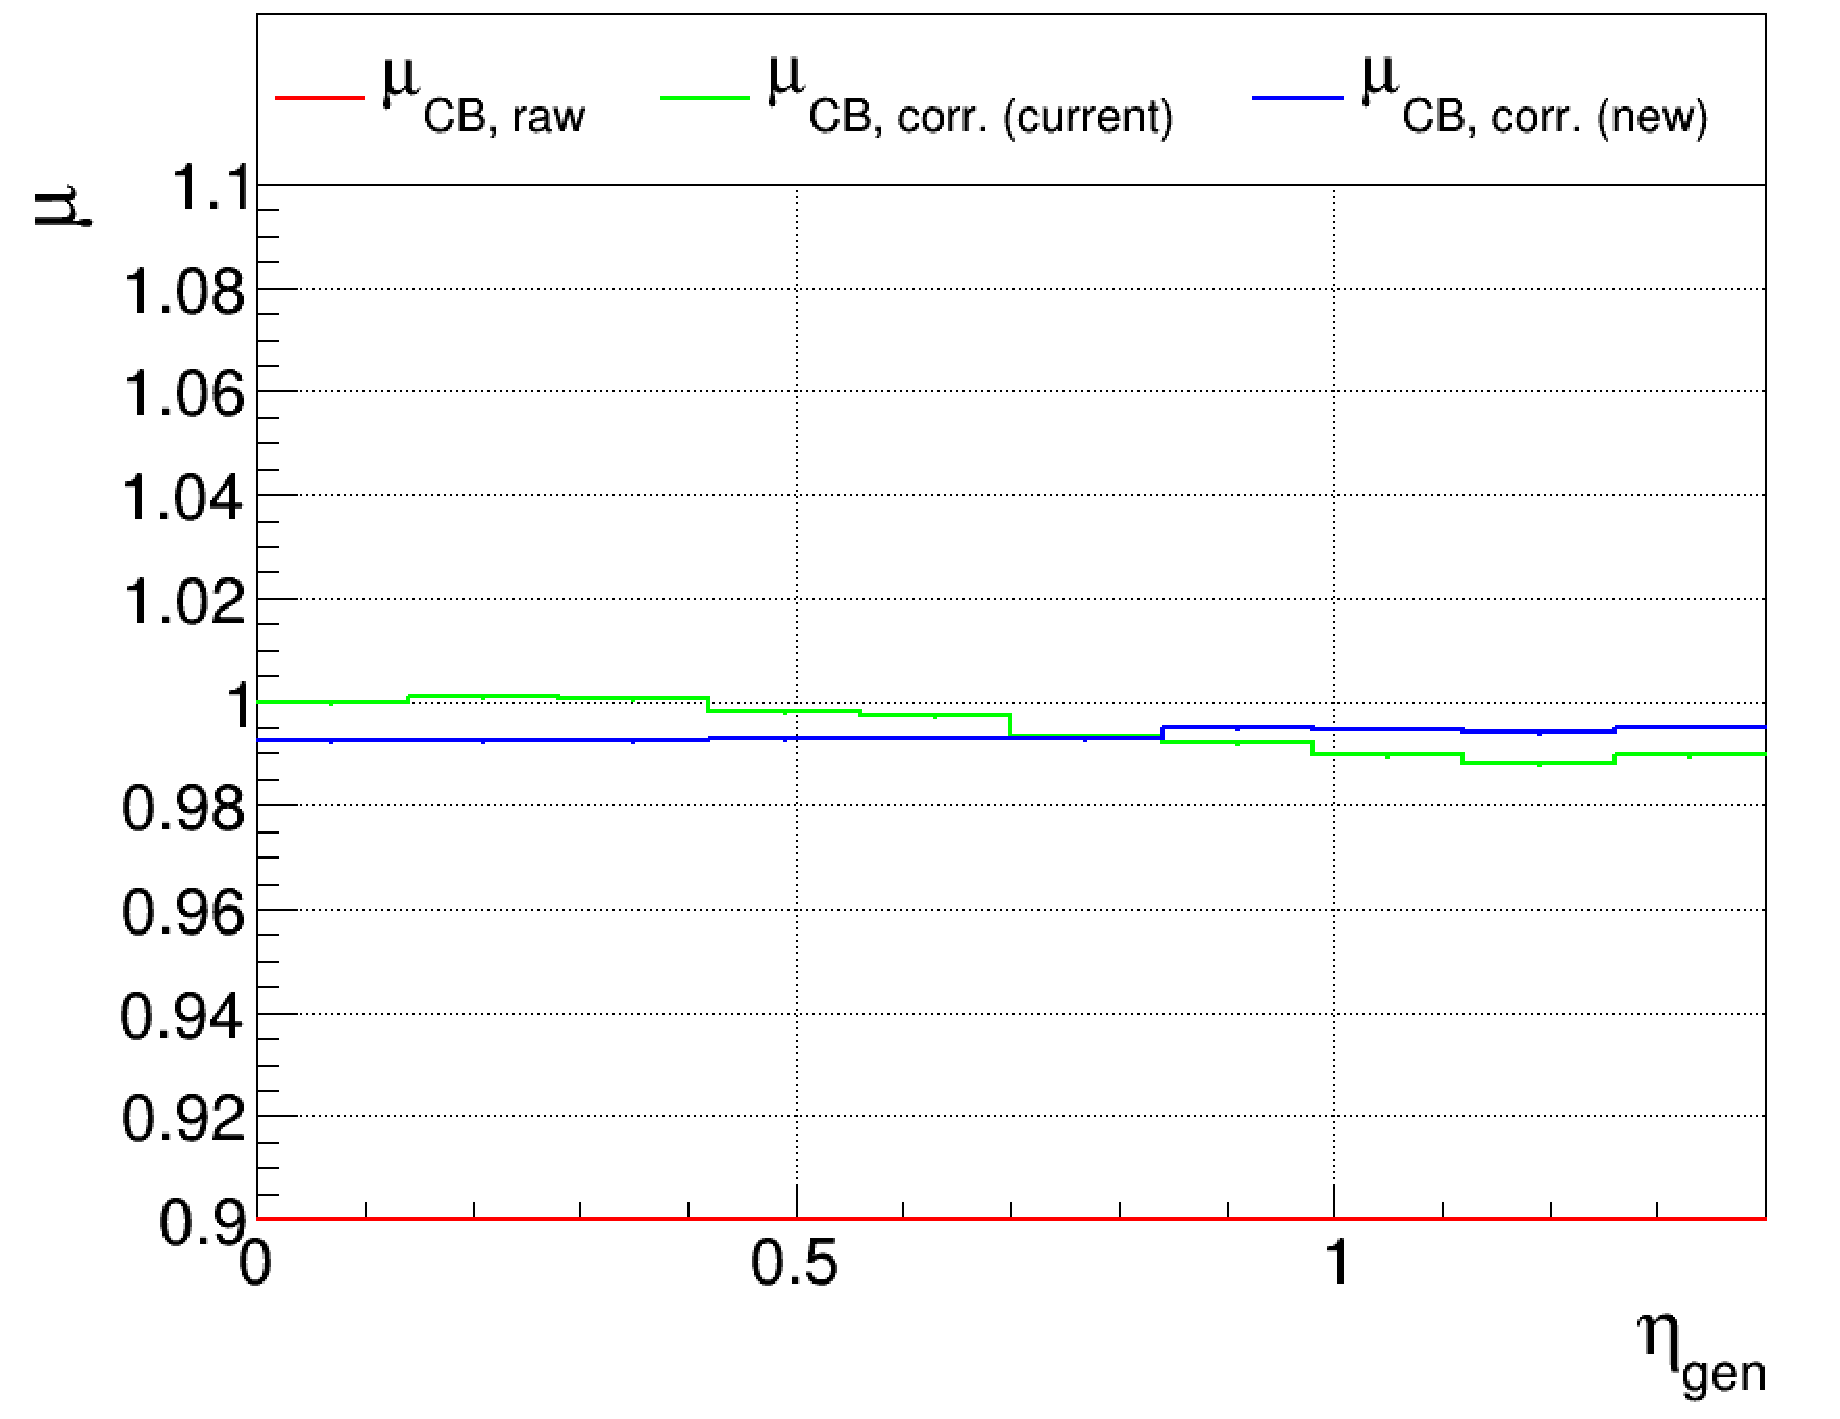
\includegraphics[width=0.495\textwidth]{./plots_pdf/ECAL_plots/plotsNOPU/EB/FULL/pdf/GENETA/EBFULL_GENETA_0005_0020_MuOverBins.pdf}
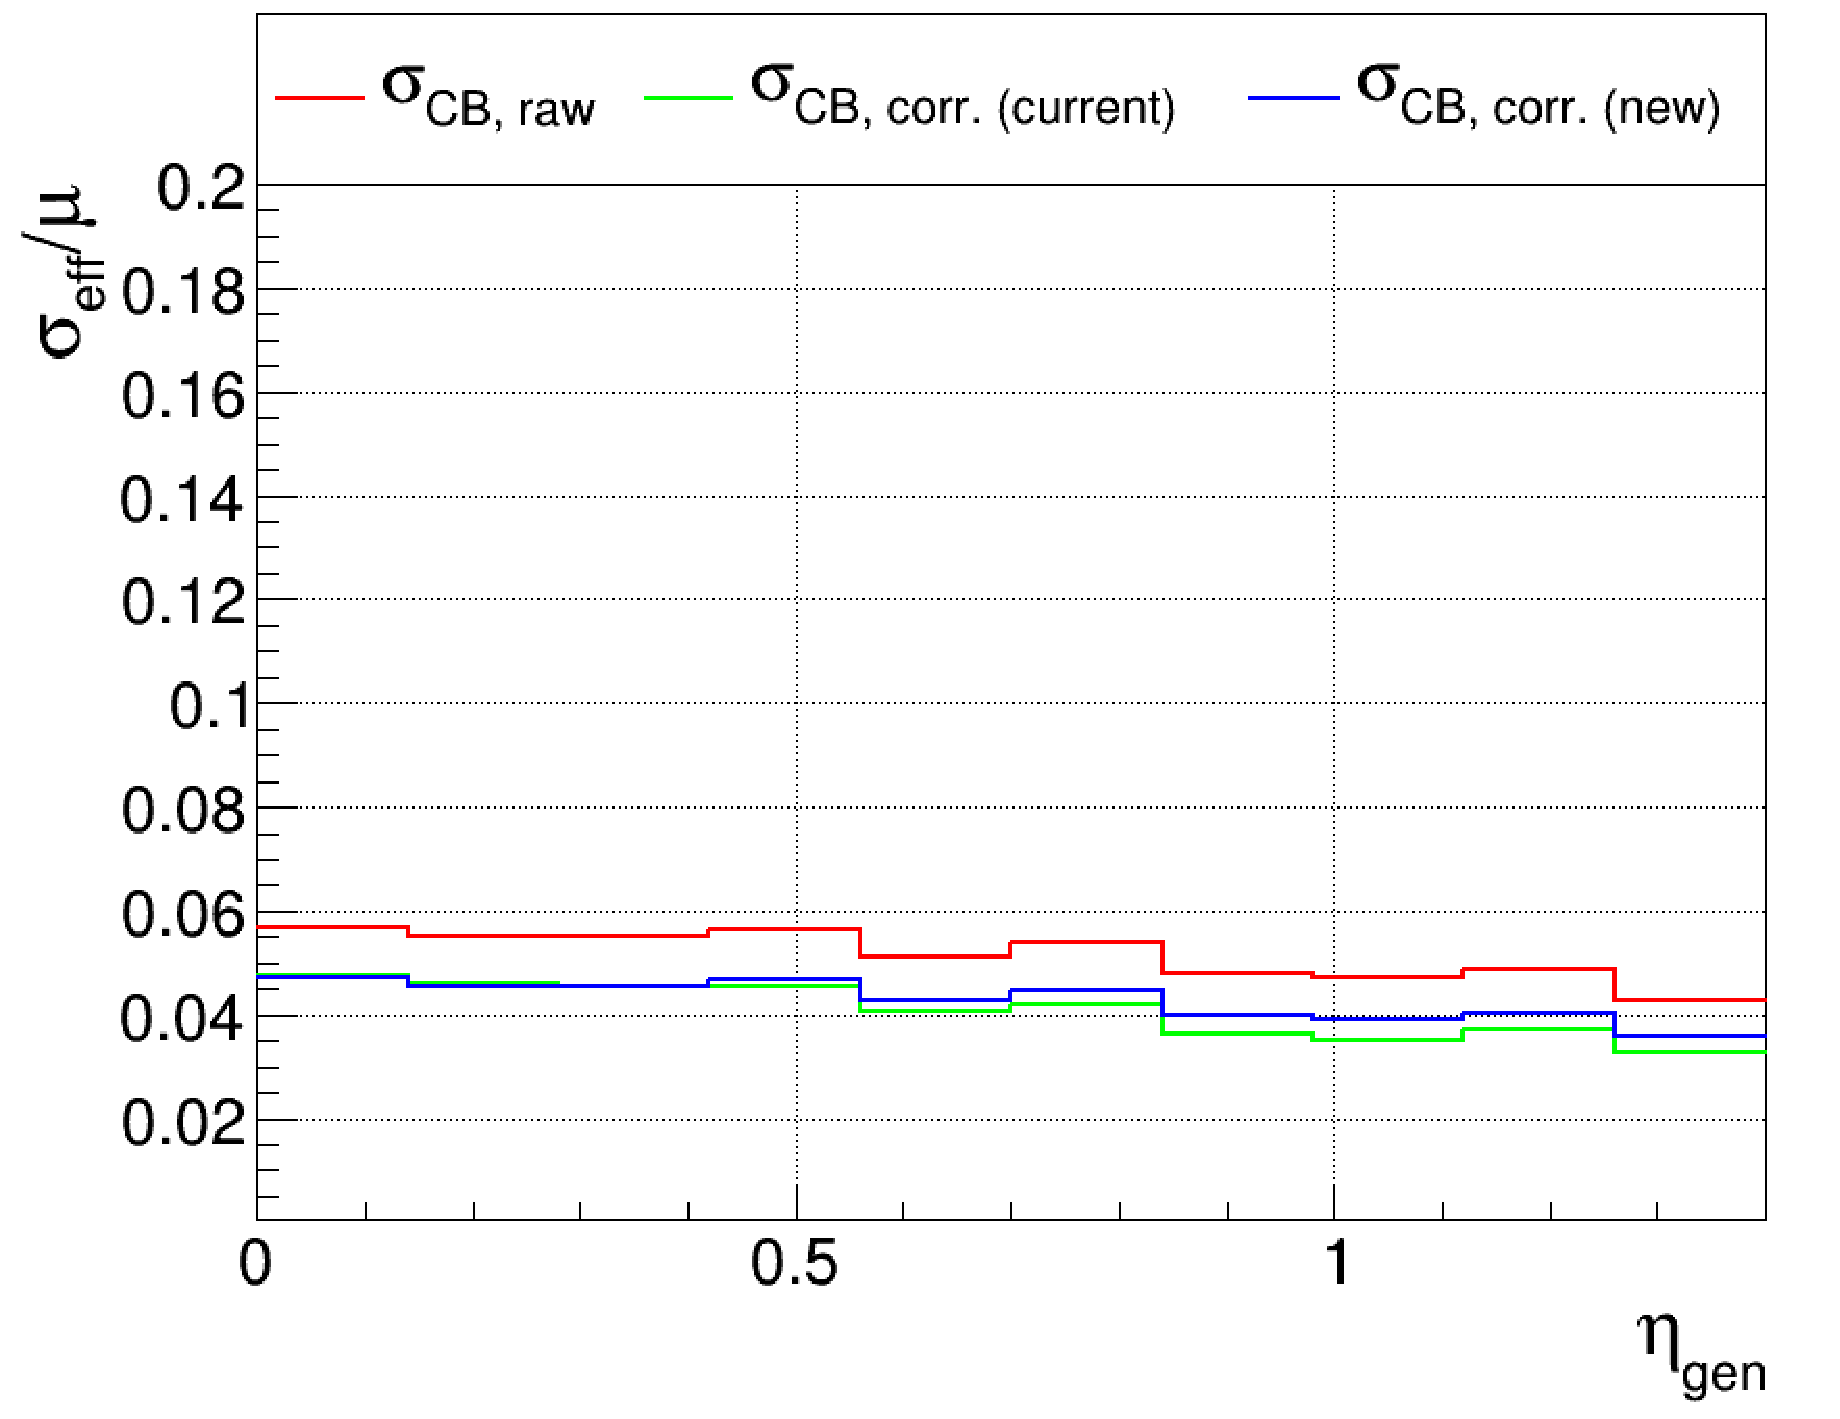
\includegraphics[width=0.495\textwidth]{./plots_pdf/ECAL_plots/plotsPU/EB/FULL/pdf/GENETA/EBFULL_GENETA_0005_0020_EffSigmaOverBins.pdf}
\caption{EB - Full Readout \pt 5-20}

%\begin{figure}
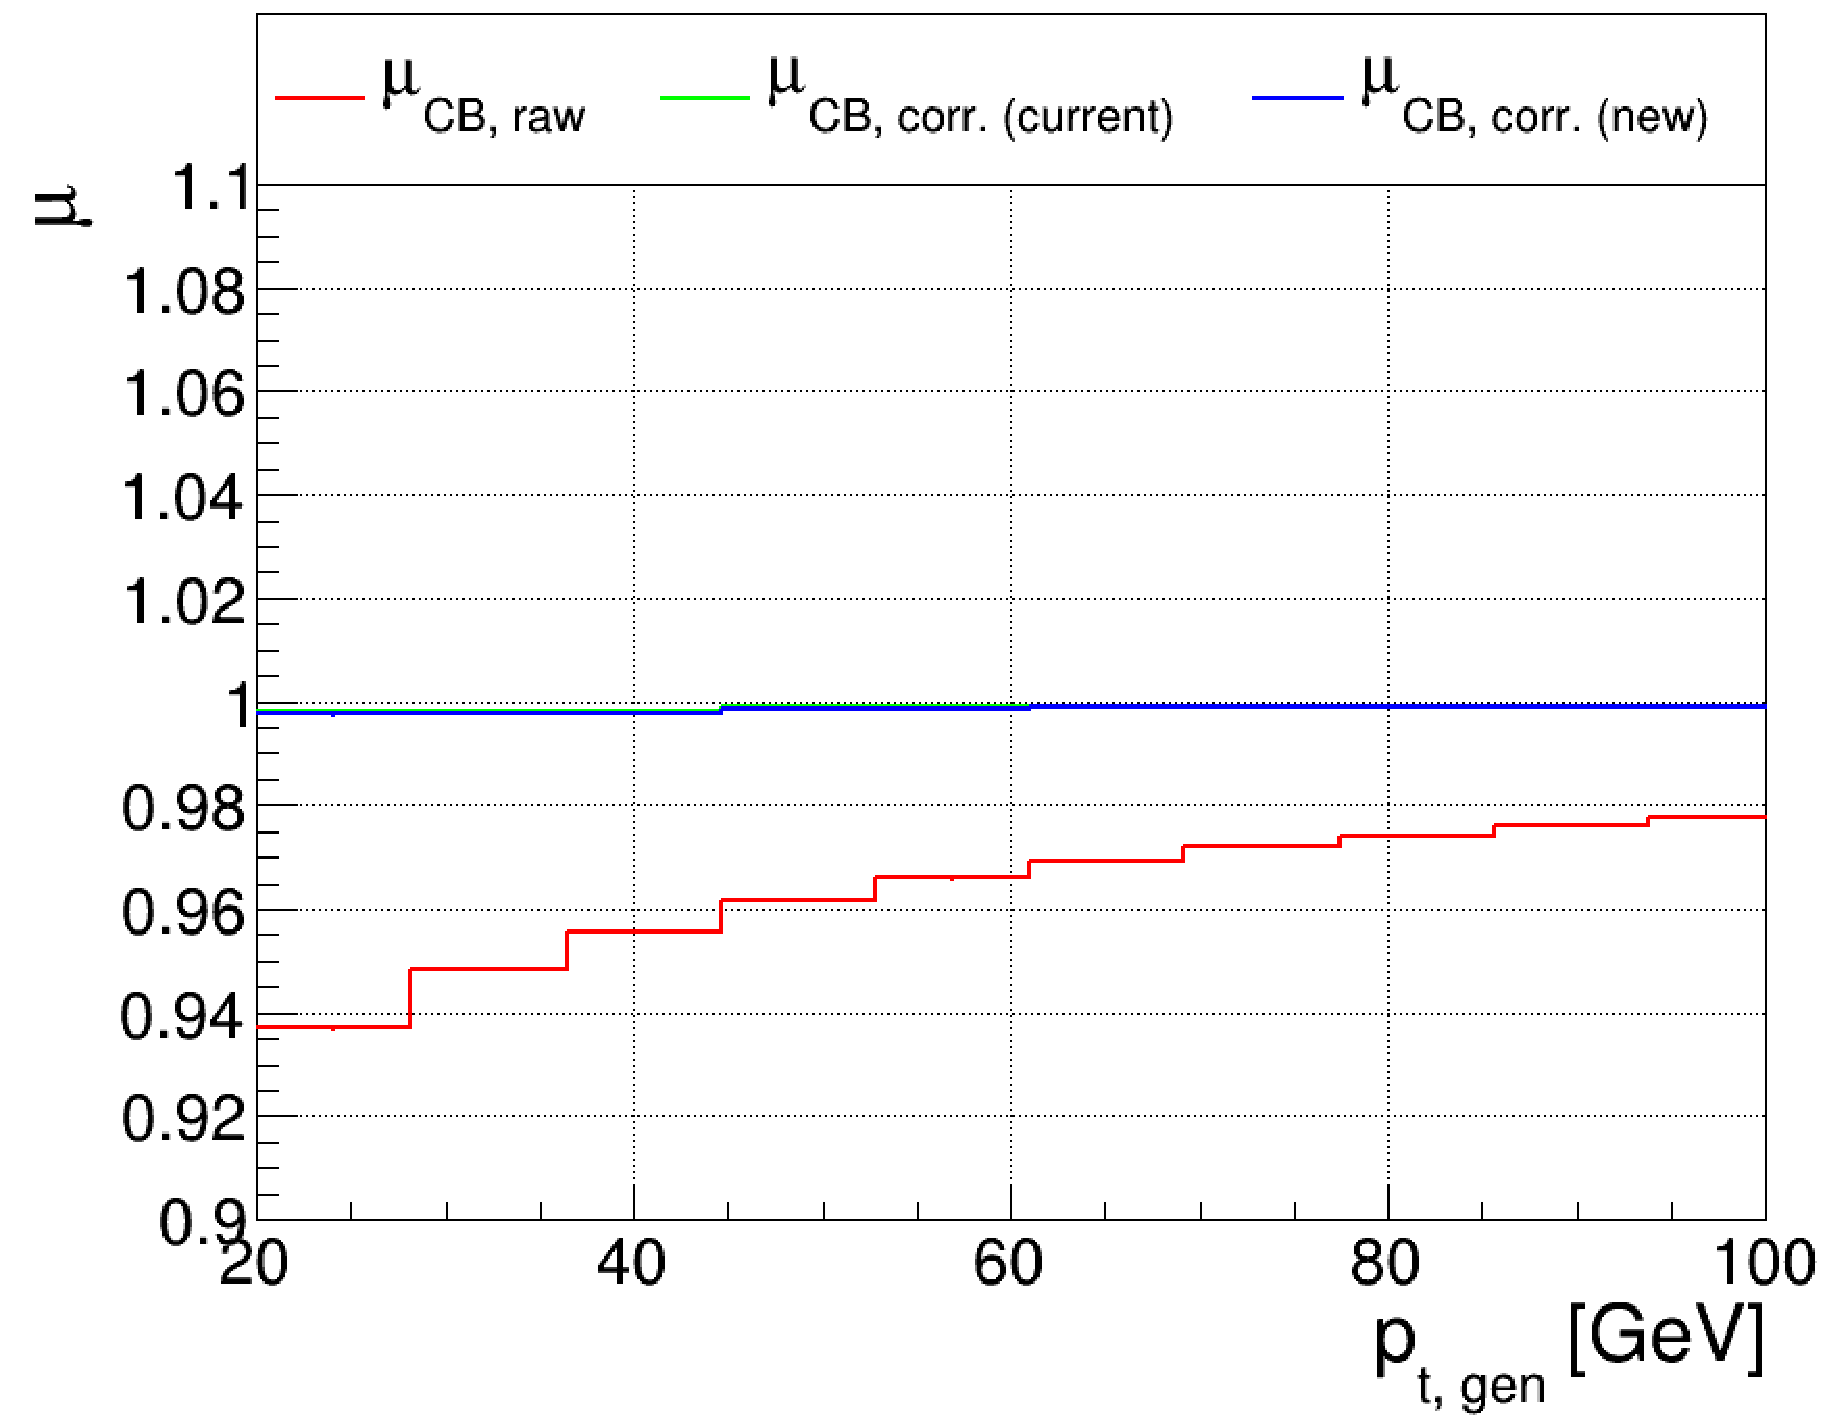
\includegraphics[width=0.495\textwidth]{./plots_pdf/ECAL_plots/plotsNOPU/EB/FULL/pdf/GENPT/EBFULL_GENPT_0020_0100_MuOverBins.pdf}
\includegraphics[width=0.495\textwidth]{./plots_pdf/ECAL_plots/plotsNOPU/EB/FULL/pdf/GENPT/EBFULL_GENPT_0020_0100_EffSigmaOverBins.pdf}

\includegraphics[width=0.495\textwidth]{./plots_pdf/ECAL_plots/plotsNOPU/EB/FULL/pdf/GENETA/EBFULL_GENETA_0020_0100_MuOverBins.pdf}
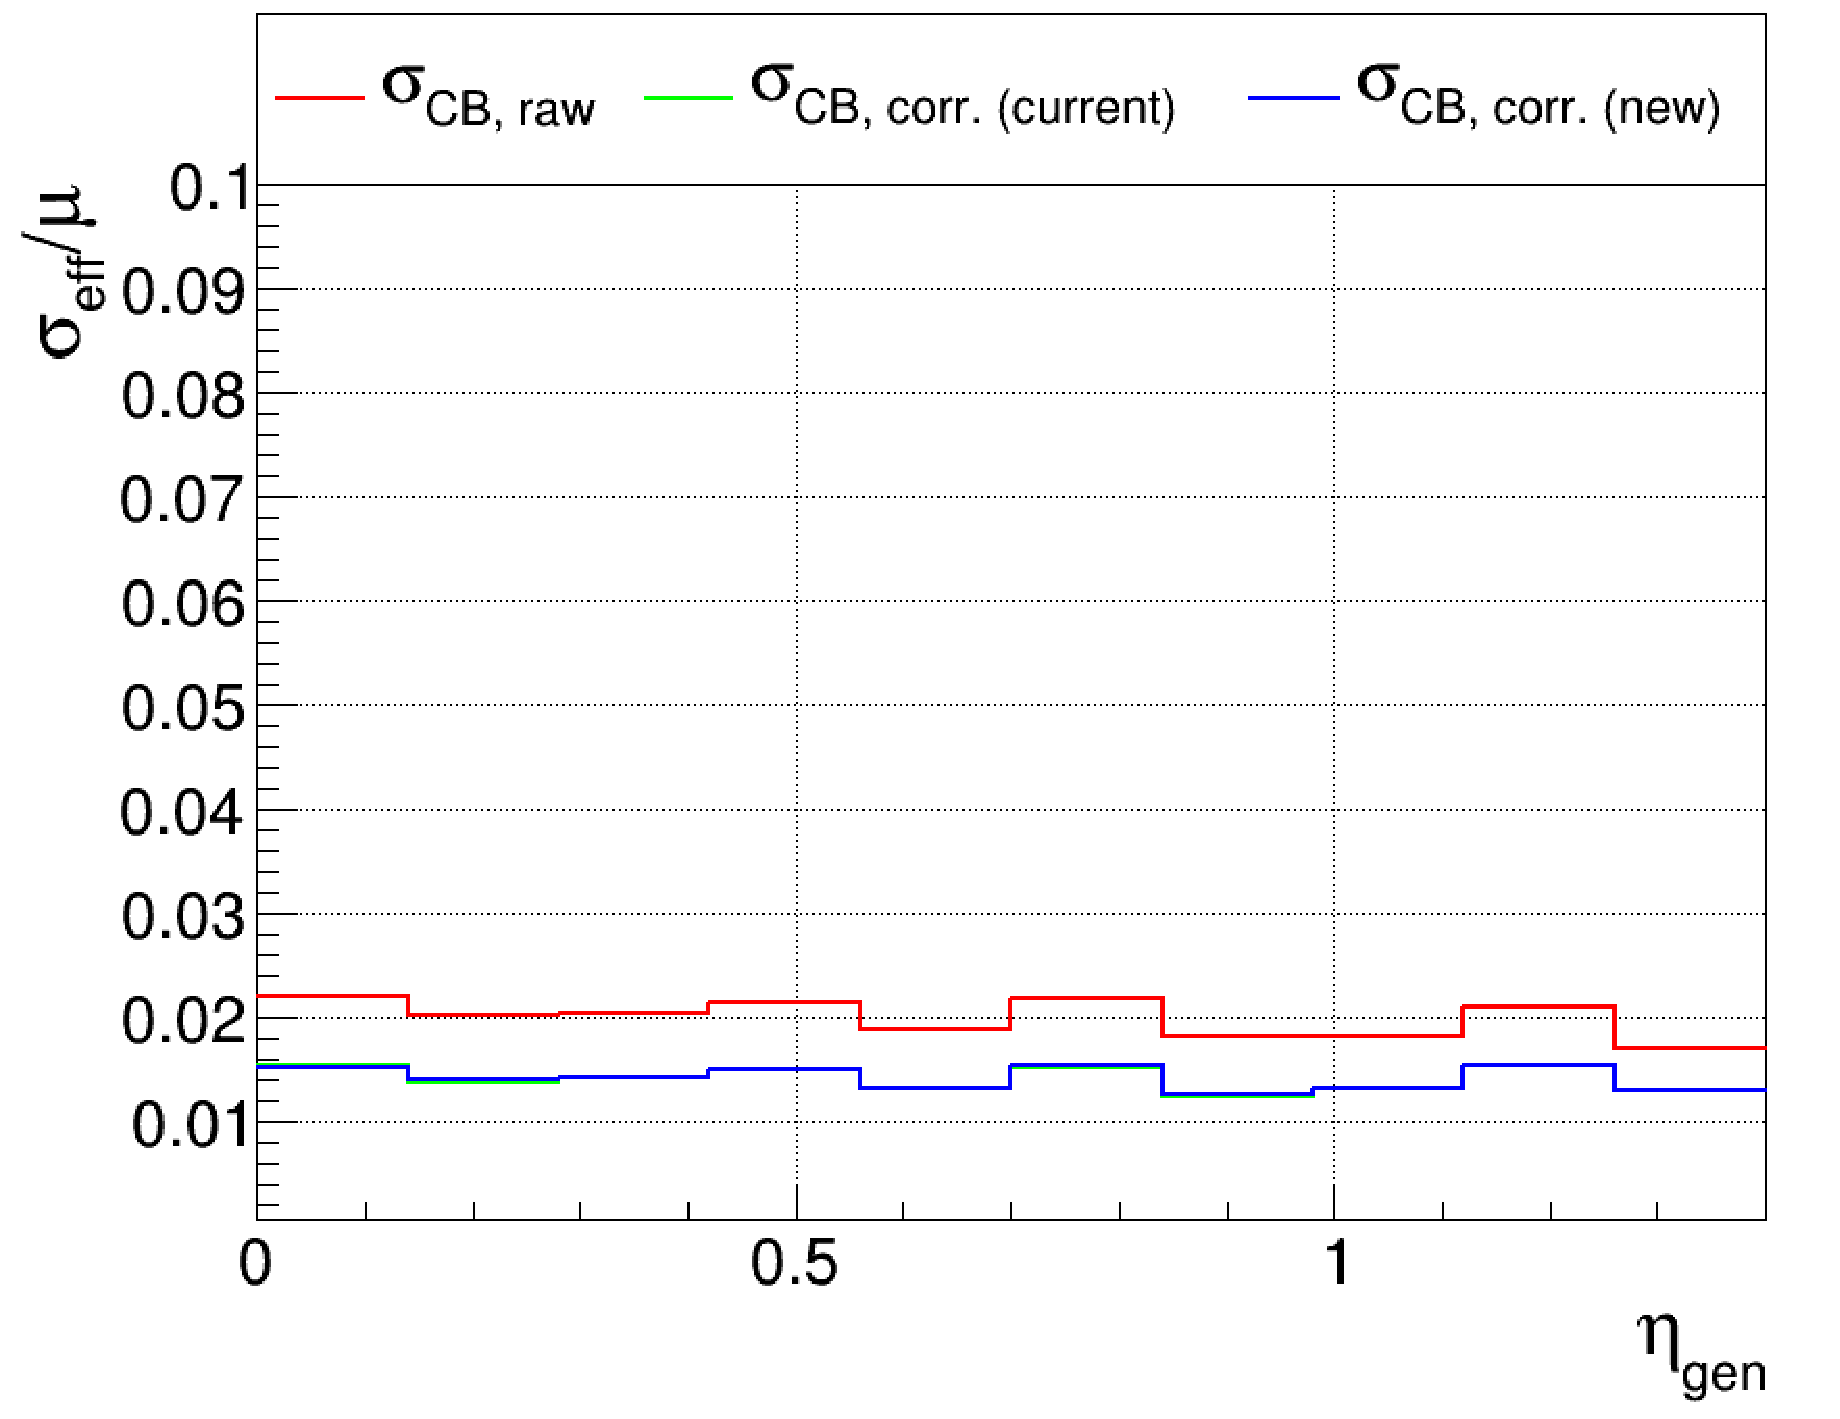
\includegraphics[width=0.495\textwidth]{./plots_pdf/ECAL_plots/plotsPU/EB/FULL/pdf/GENETA/EBFULL_GENETA_0020_0100_EffSigmaOverBins.pdf}
\caption{EB - Full Readout \pt 20-100}
\end{figure}


\begin{figure}
\includegraphics[width=0.495\textwidth]{./plots_pdf/ECAL_plots/plotsNOPU/EB/FULL/pdf/GENPT/EBFULL_GENPT_0100_0300_MuOverBins.pdf}
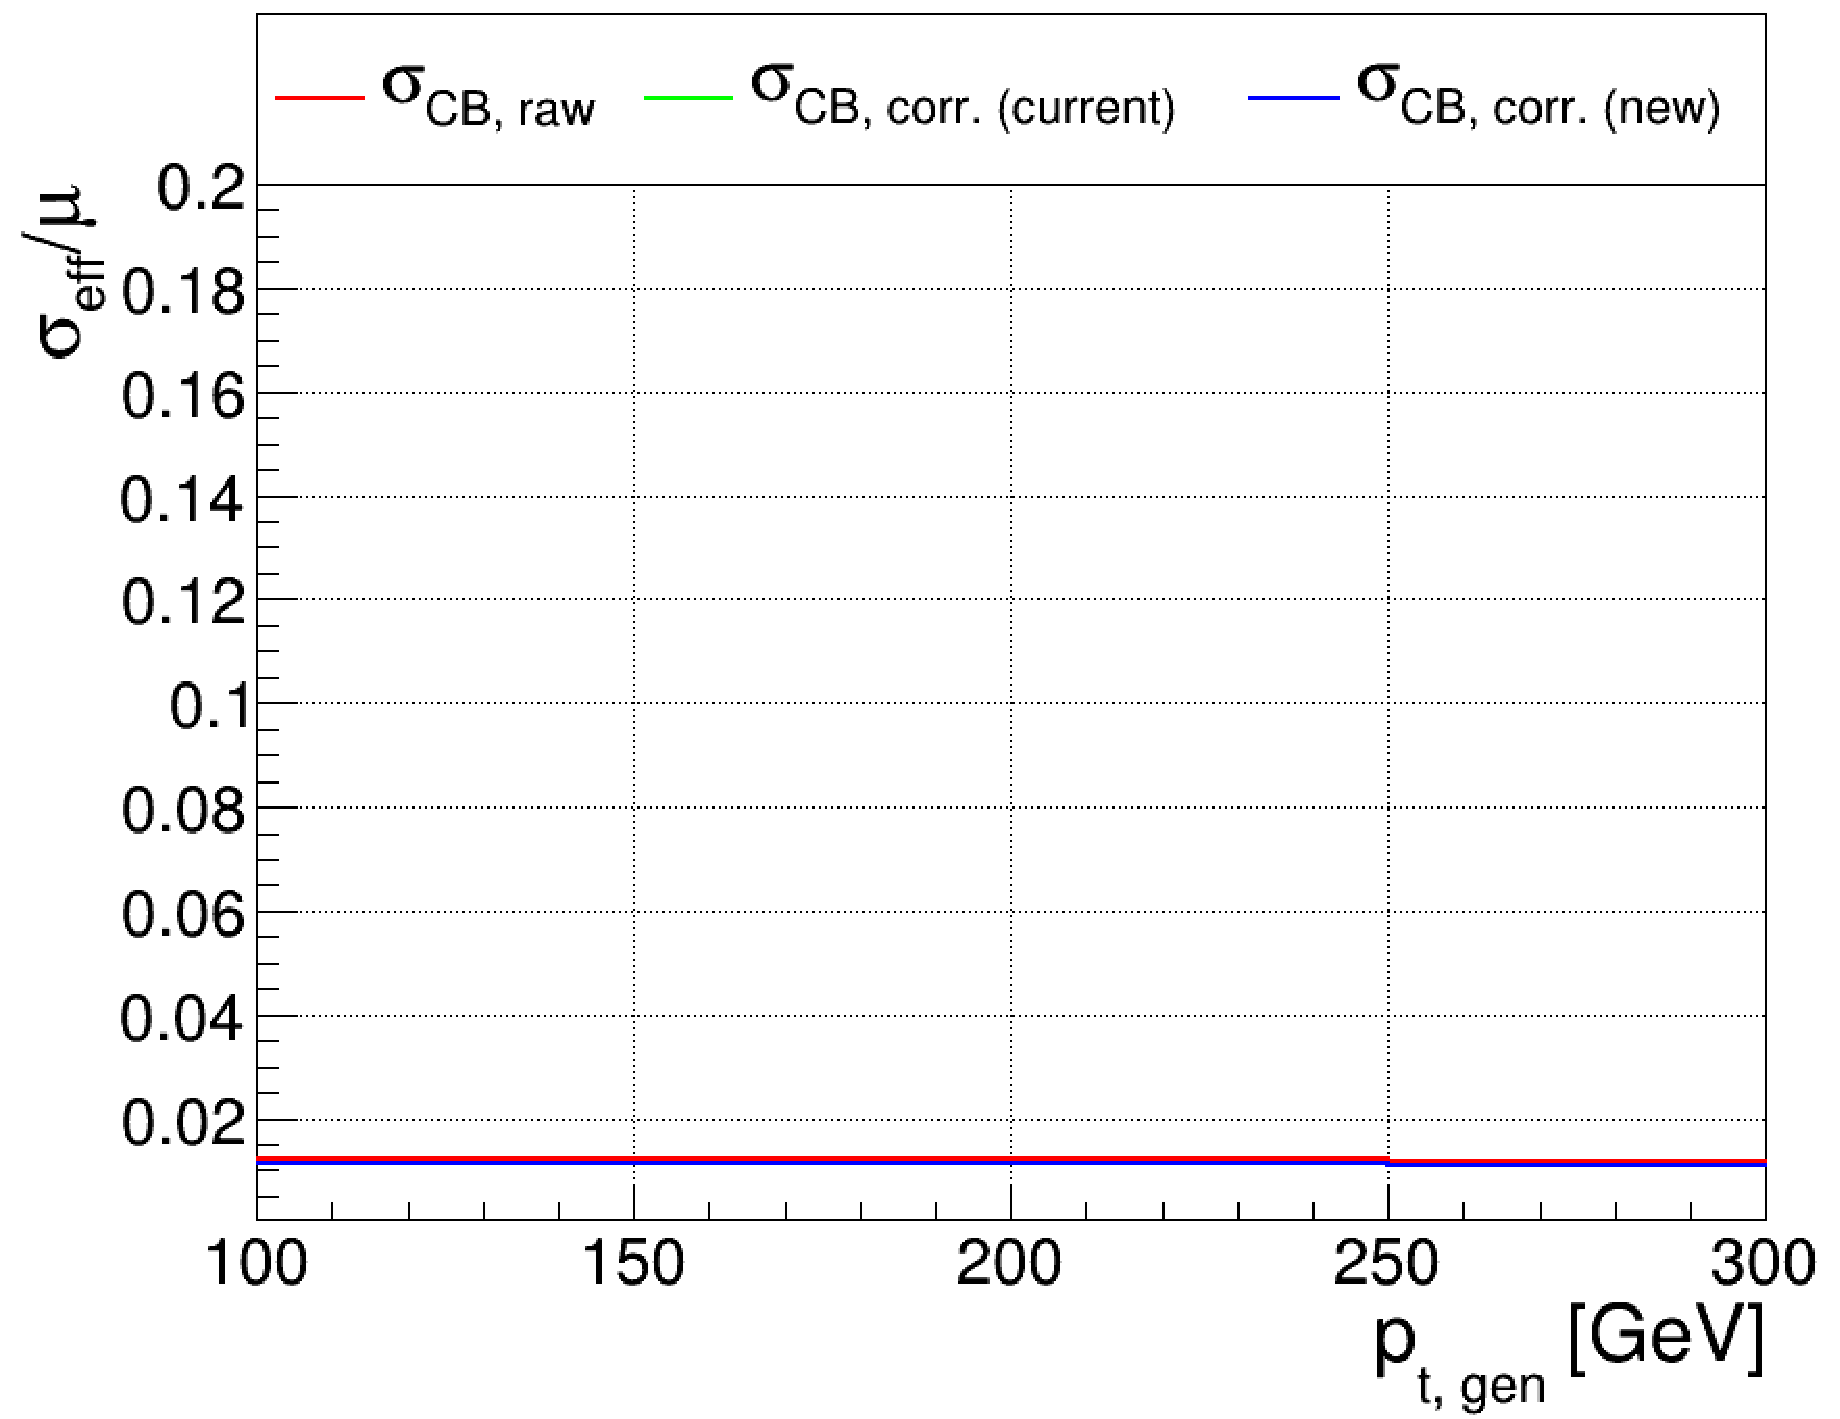
\includegraphics[width=0.495\textwidth]{./plots_pdf/ECAL_plots/plotsPU/EB/FULL/pdf/GENPT/EBFULL_GENPT_0100_0300_EffSigmaOverBins.pdf}


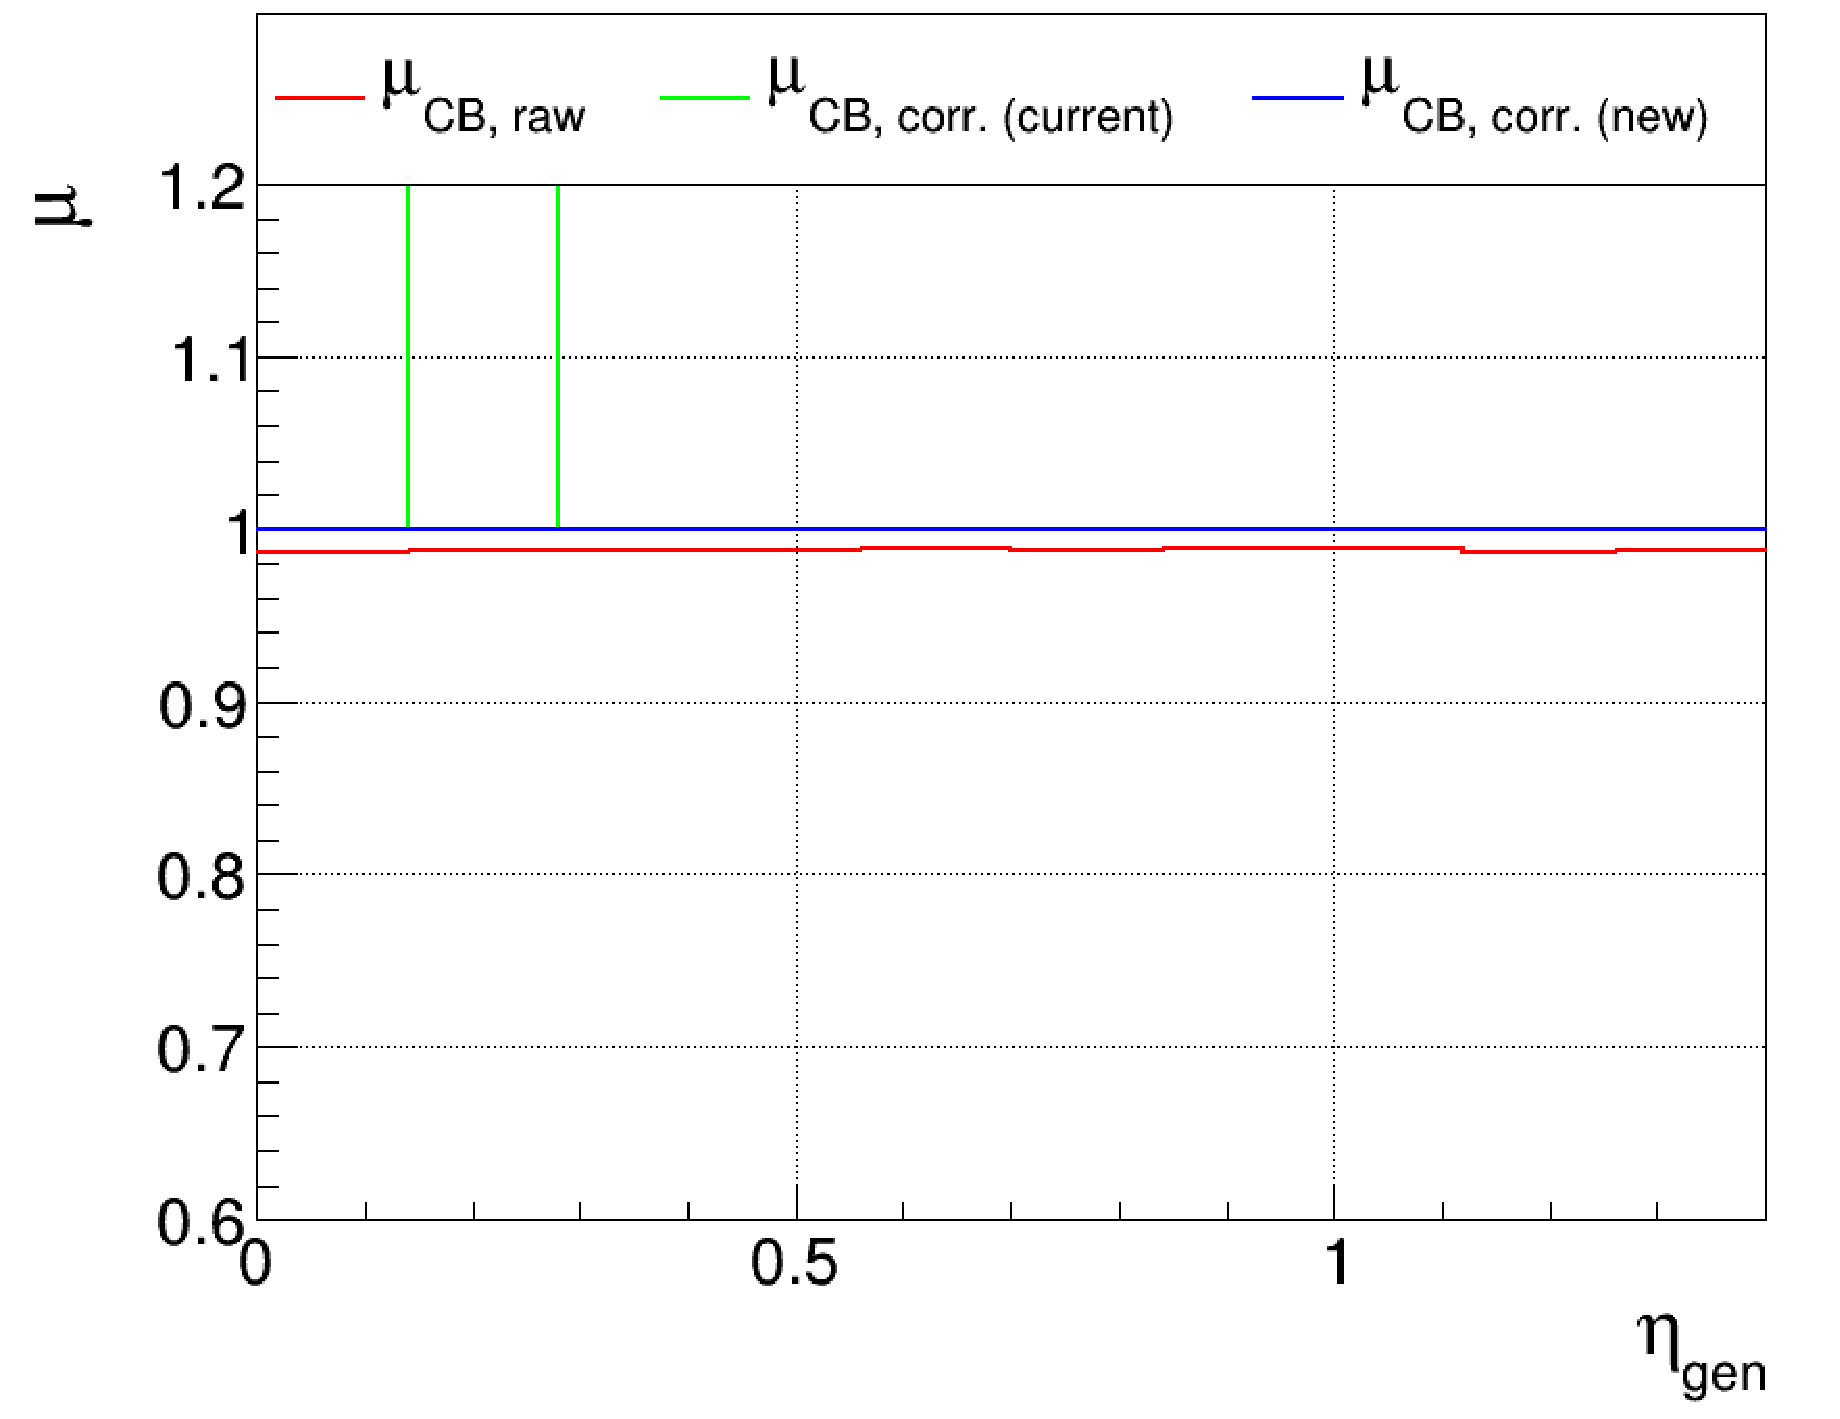
\includegraphics[width=0.495\textwidth]{./plots_pdf/ECAL_plots/plotsNOPU/EB/FULL/pdf/GENETA/EBFULL_GENETA_0100_0300_MuOverBins.pdf}
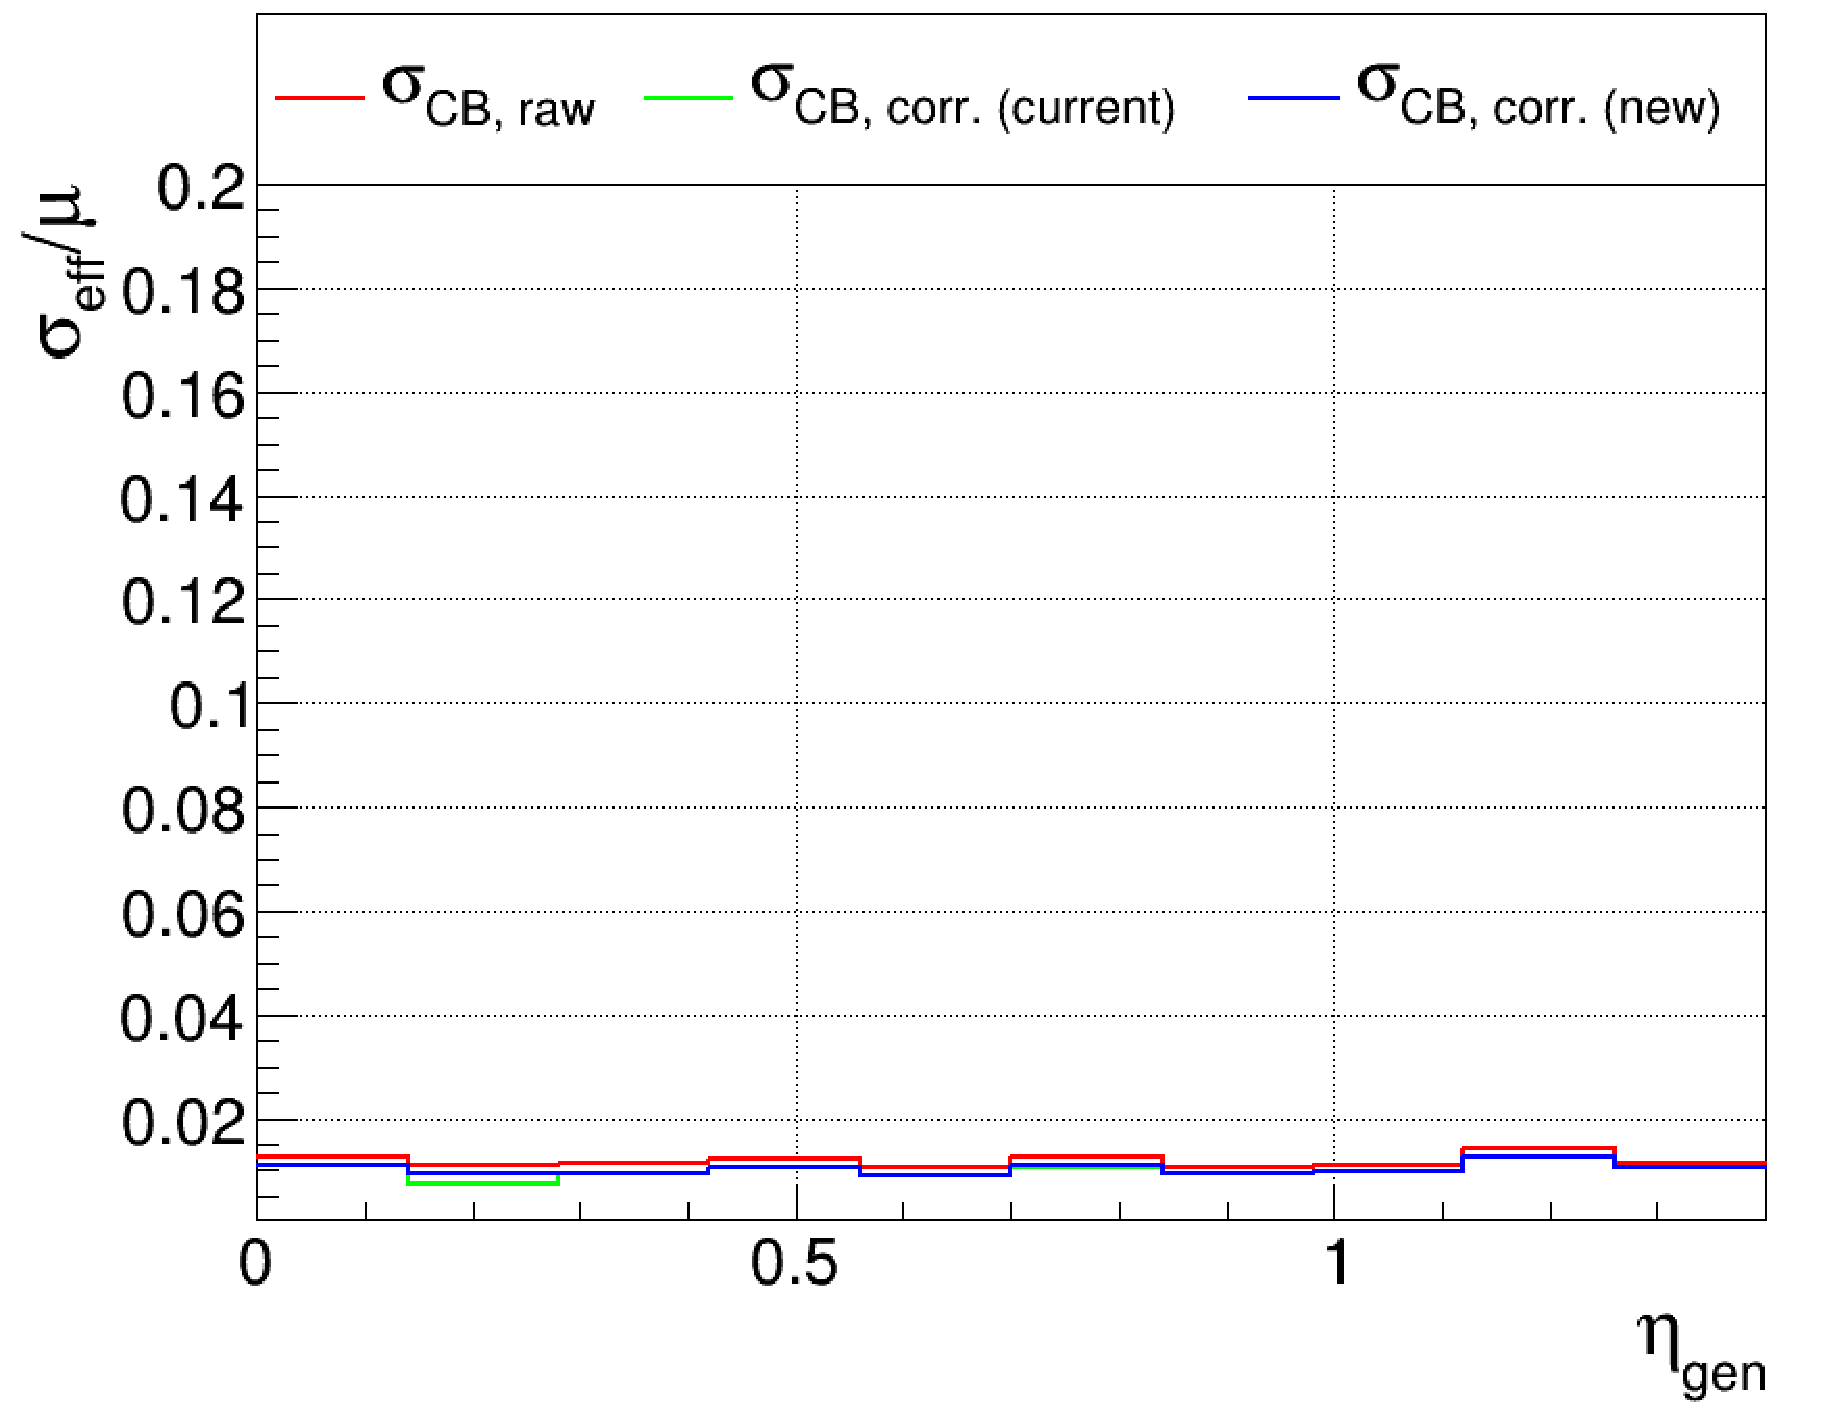
\includegraphics[width=0.495\textwidth]{./plots_pdf/ECAL_plots/plotsNOPU/EB/FULL/pdf/GENETA/EBFULL_GENETA_0100_0300_EffSigmaOverBins.pdf}
\caption{EB - Full Readout \pt 100-300}
\end{figure}




\begin{figure}
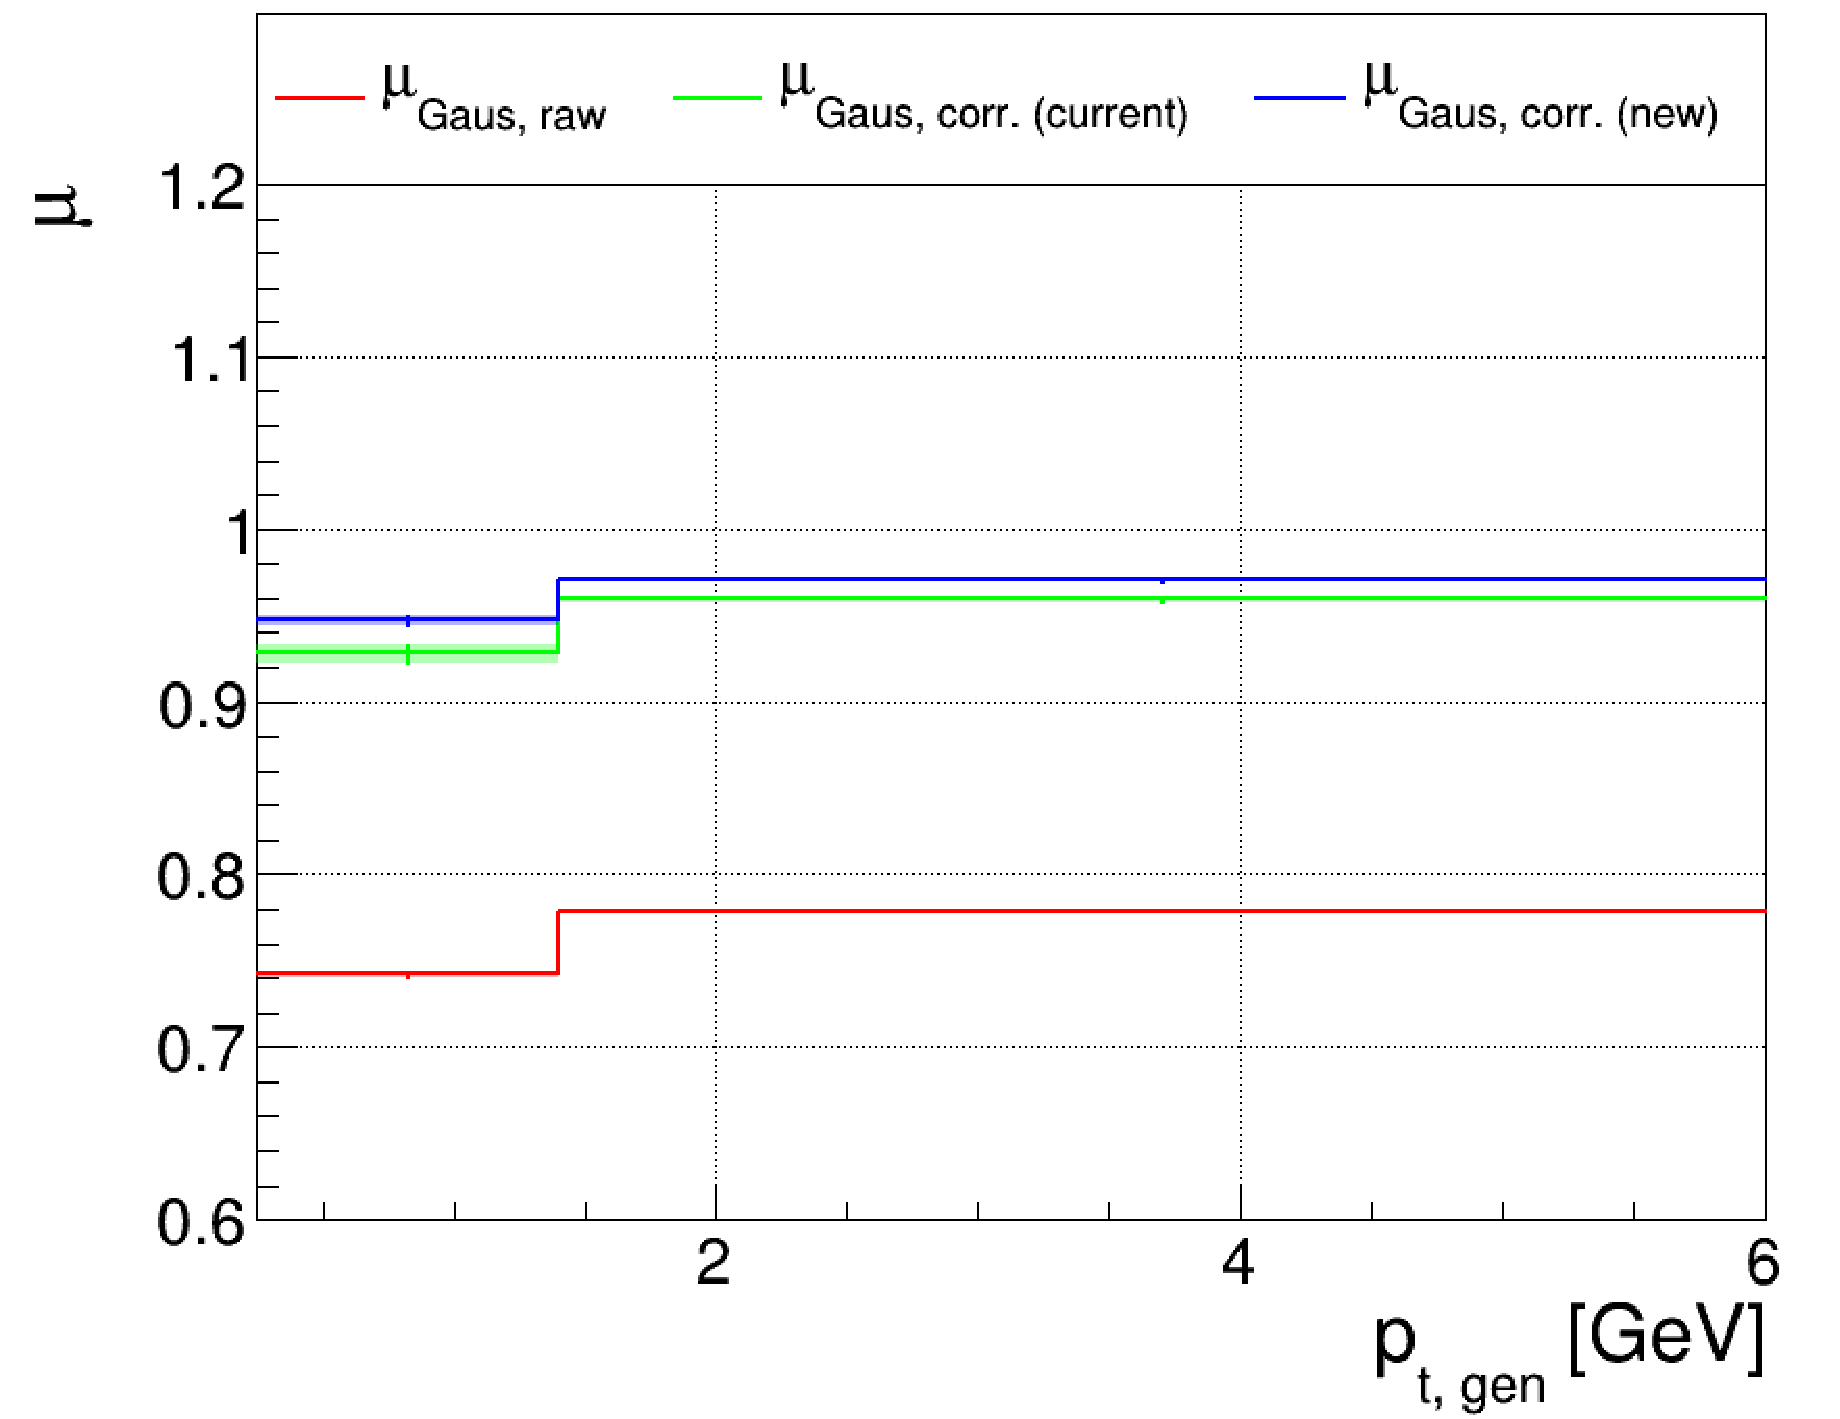
\includegraphics[width=0.495\textwidth]{./ECAL_plots/plotsNOPU/EB/ZS/pdf/GENPT/EBZS_GENPT_0000_0006_MuOverBins.pdf}
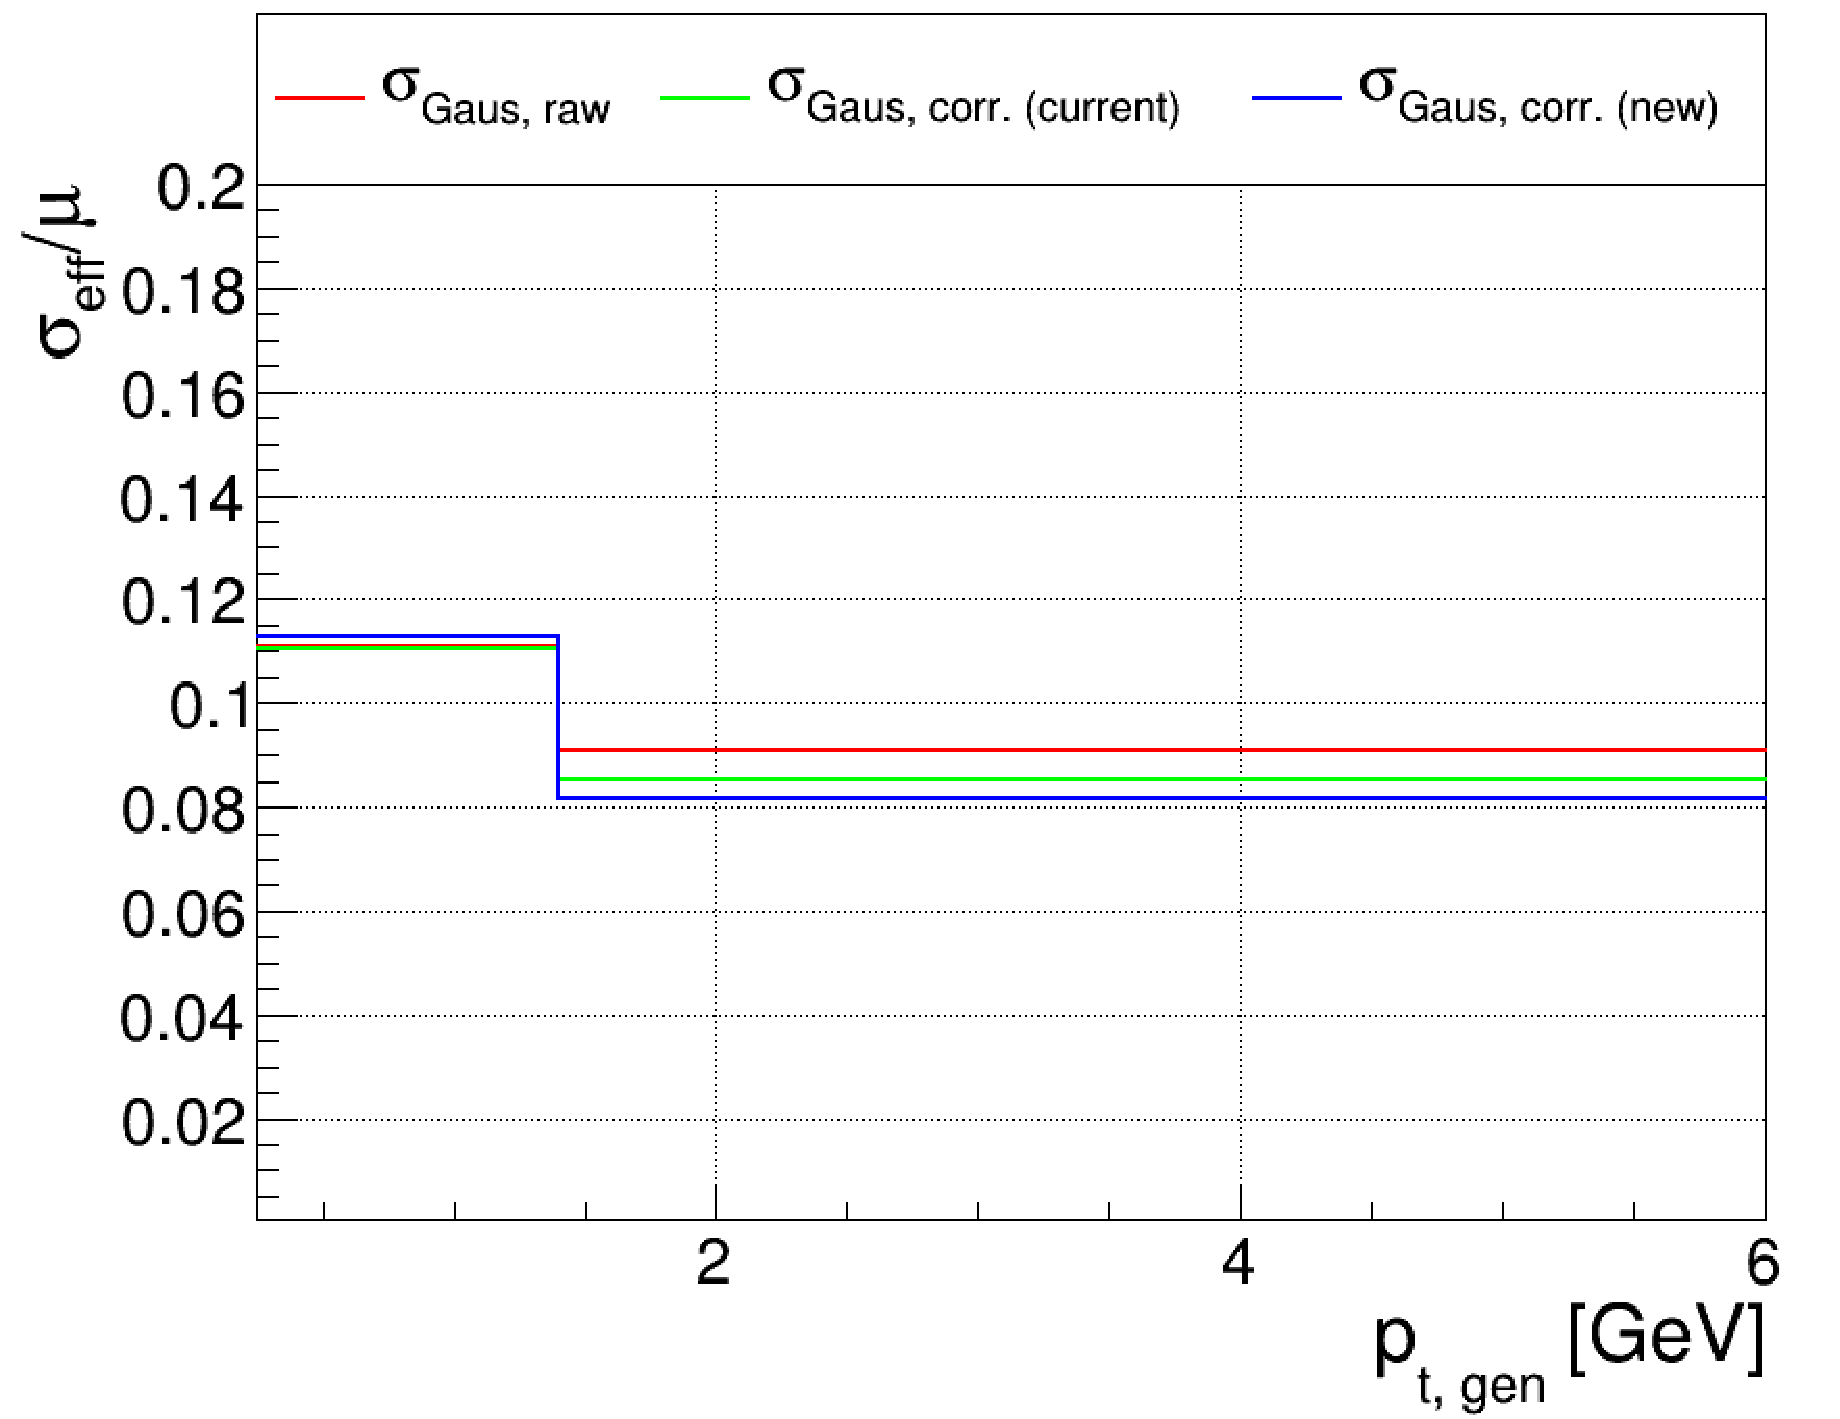
\includegraphics[width=0.495\textwidth]{./ECAL_plots/plotsNOPU/EB/ZS/pdf/GENPT/EBZS_GENPT_0000_0006_EffSigmaOverBins.pdf}
%\caption{EB - ZSl Readout pt 0-6}
%\end{figure}
%\begin{figure}
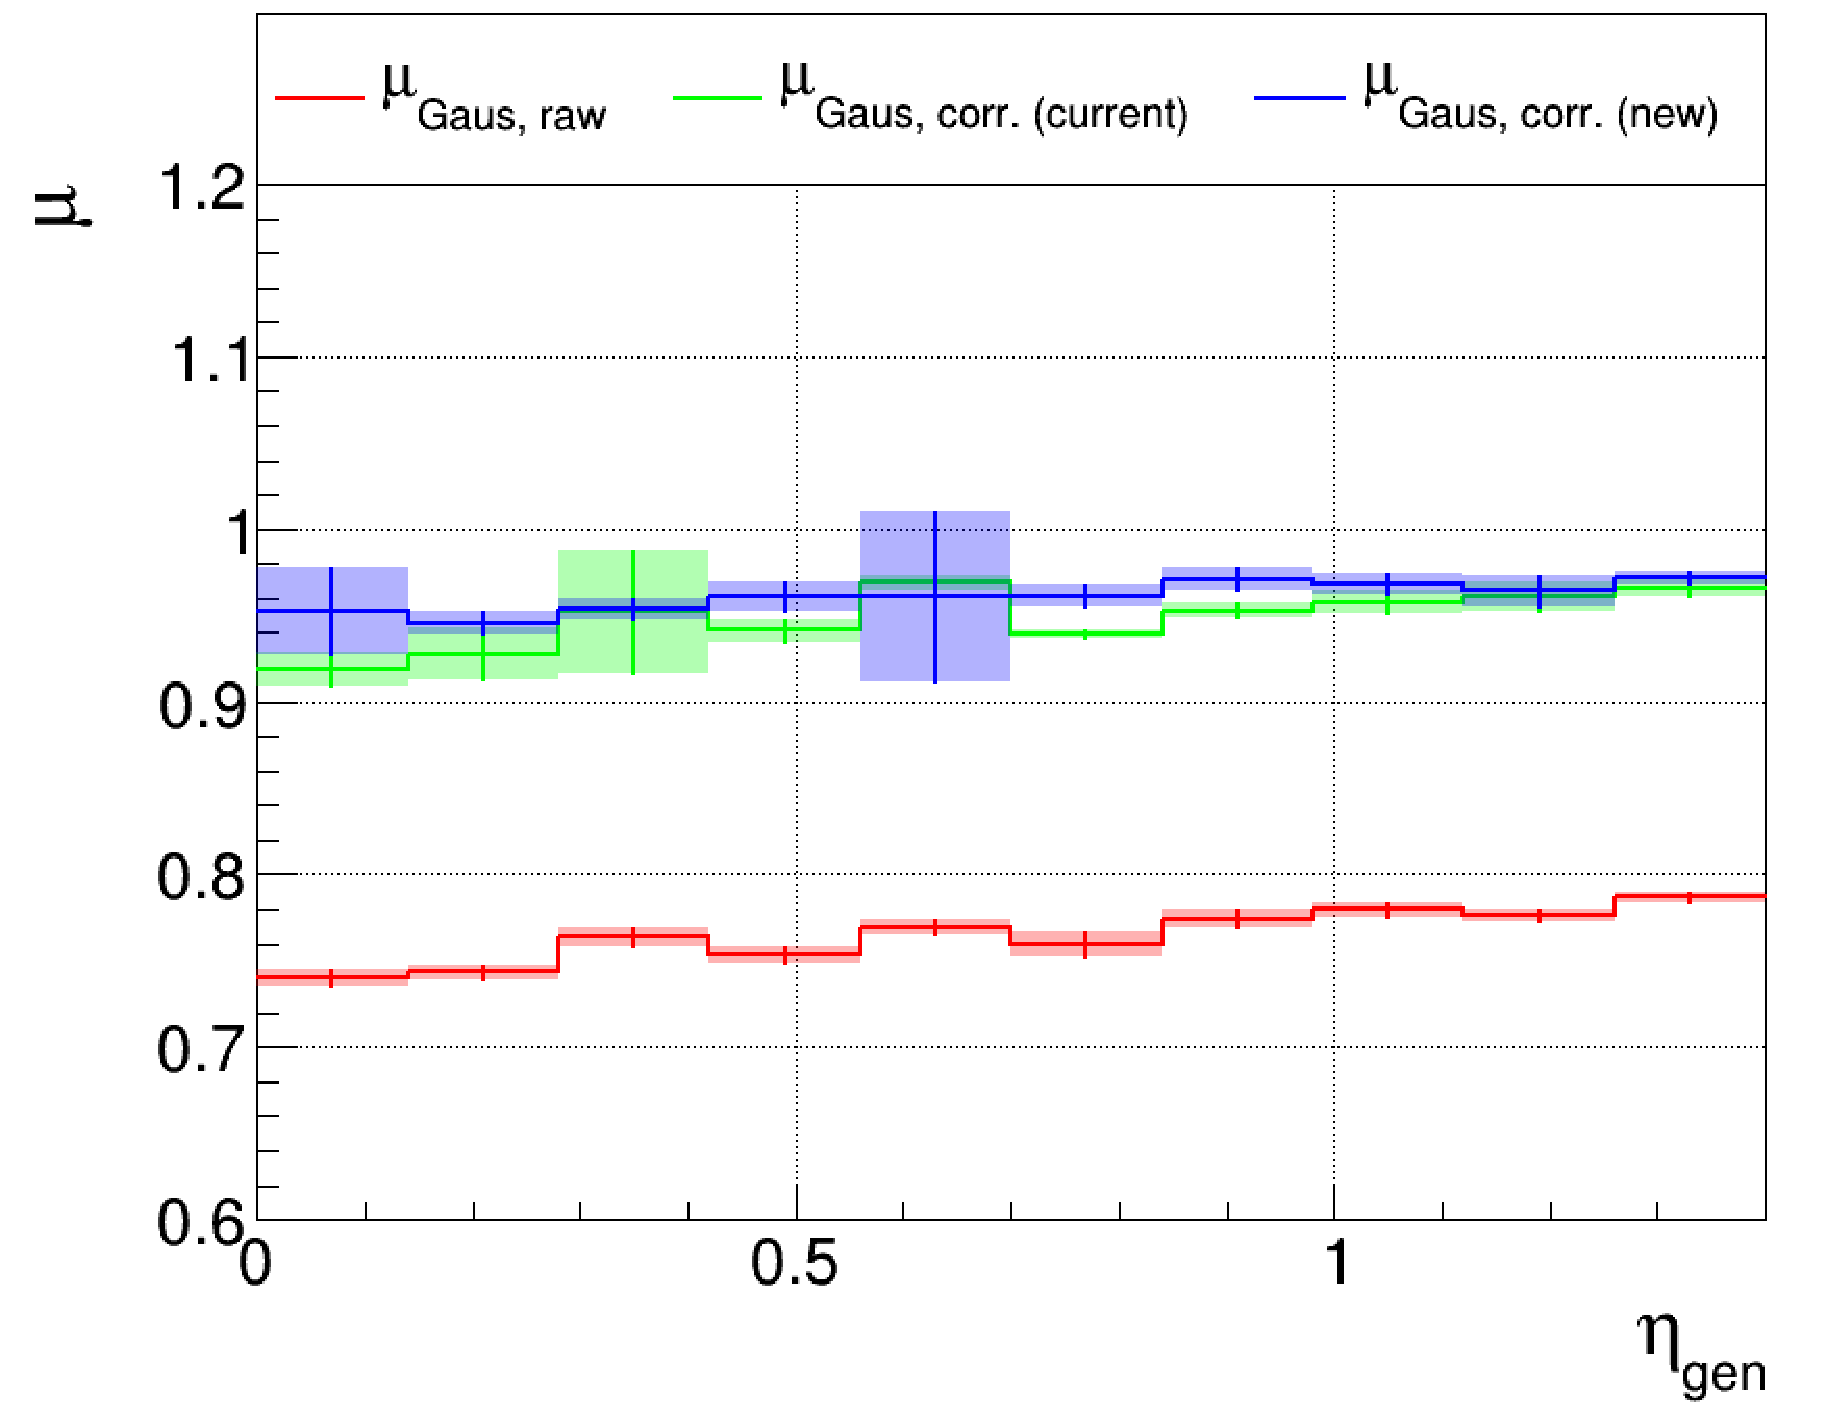
\includegraphics[width=0.495\textwidth]{./ECAL_plots/plotsNOPU/EB/ZS/pdf/GENETA/EBZS_GENETA_0000_0006_MuOverBins.pdf}
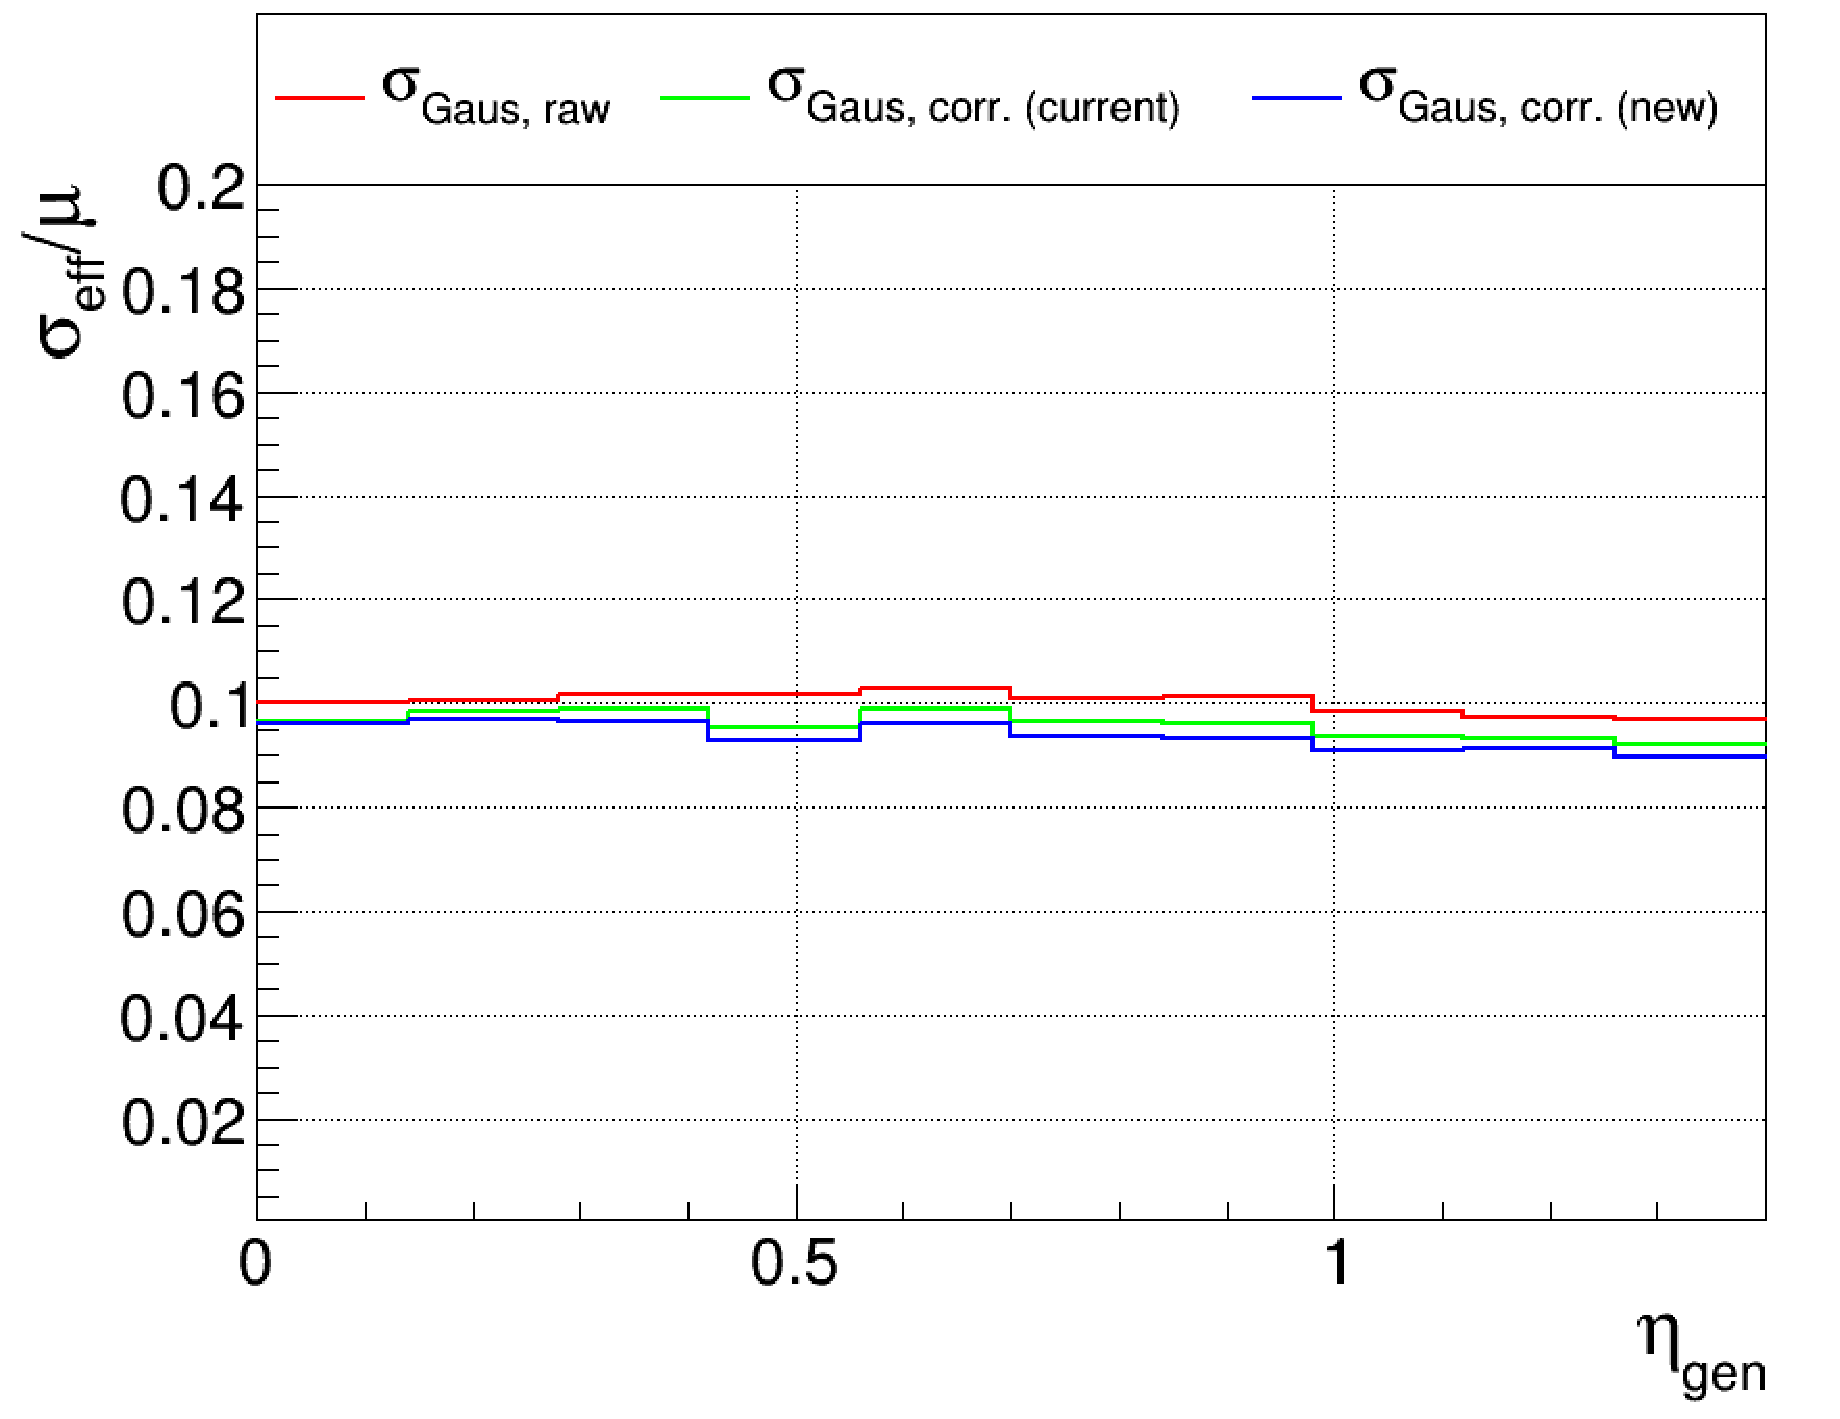
\includegraphics[width=0.495\textwidth]{./ECAL_plots/plotsNOPU/EB/ZS/pdf/GENETA/EBZS_GENETA_0000_0006_EffSigmaOverBins.pdf}
\caption{EB - ZS Readout pt 0-6}
\end{figure}


\begin{figure}
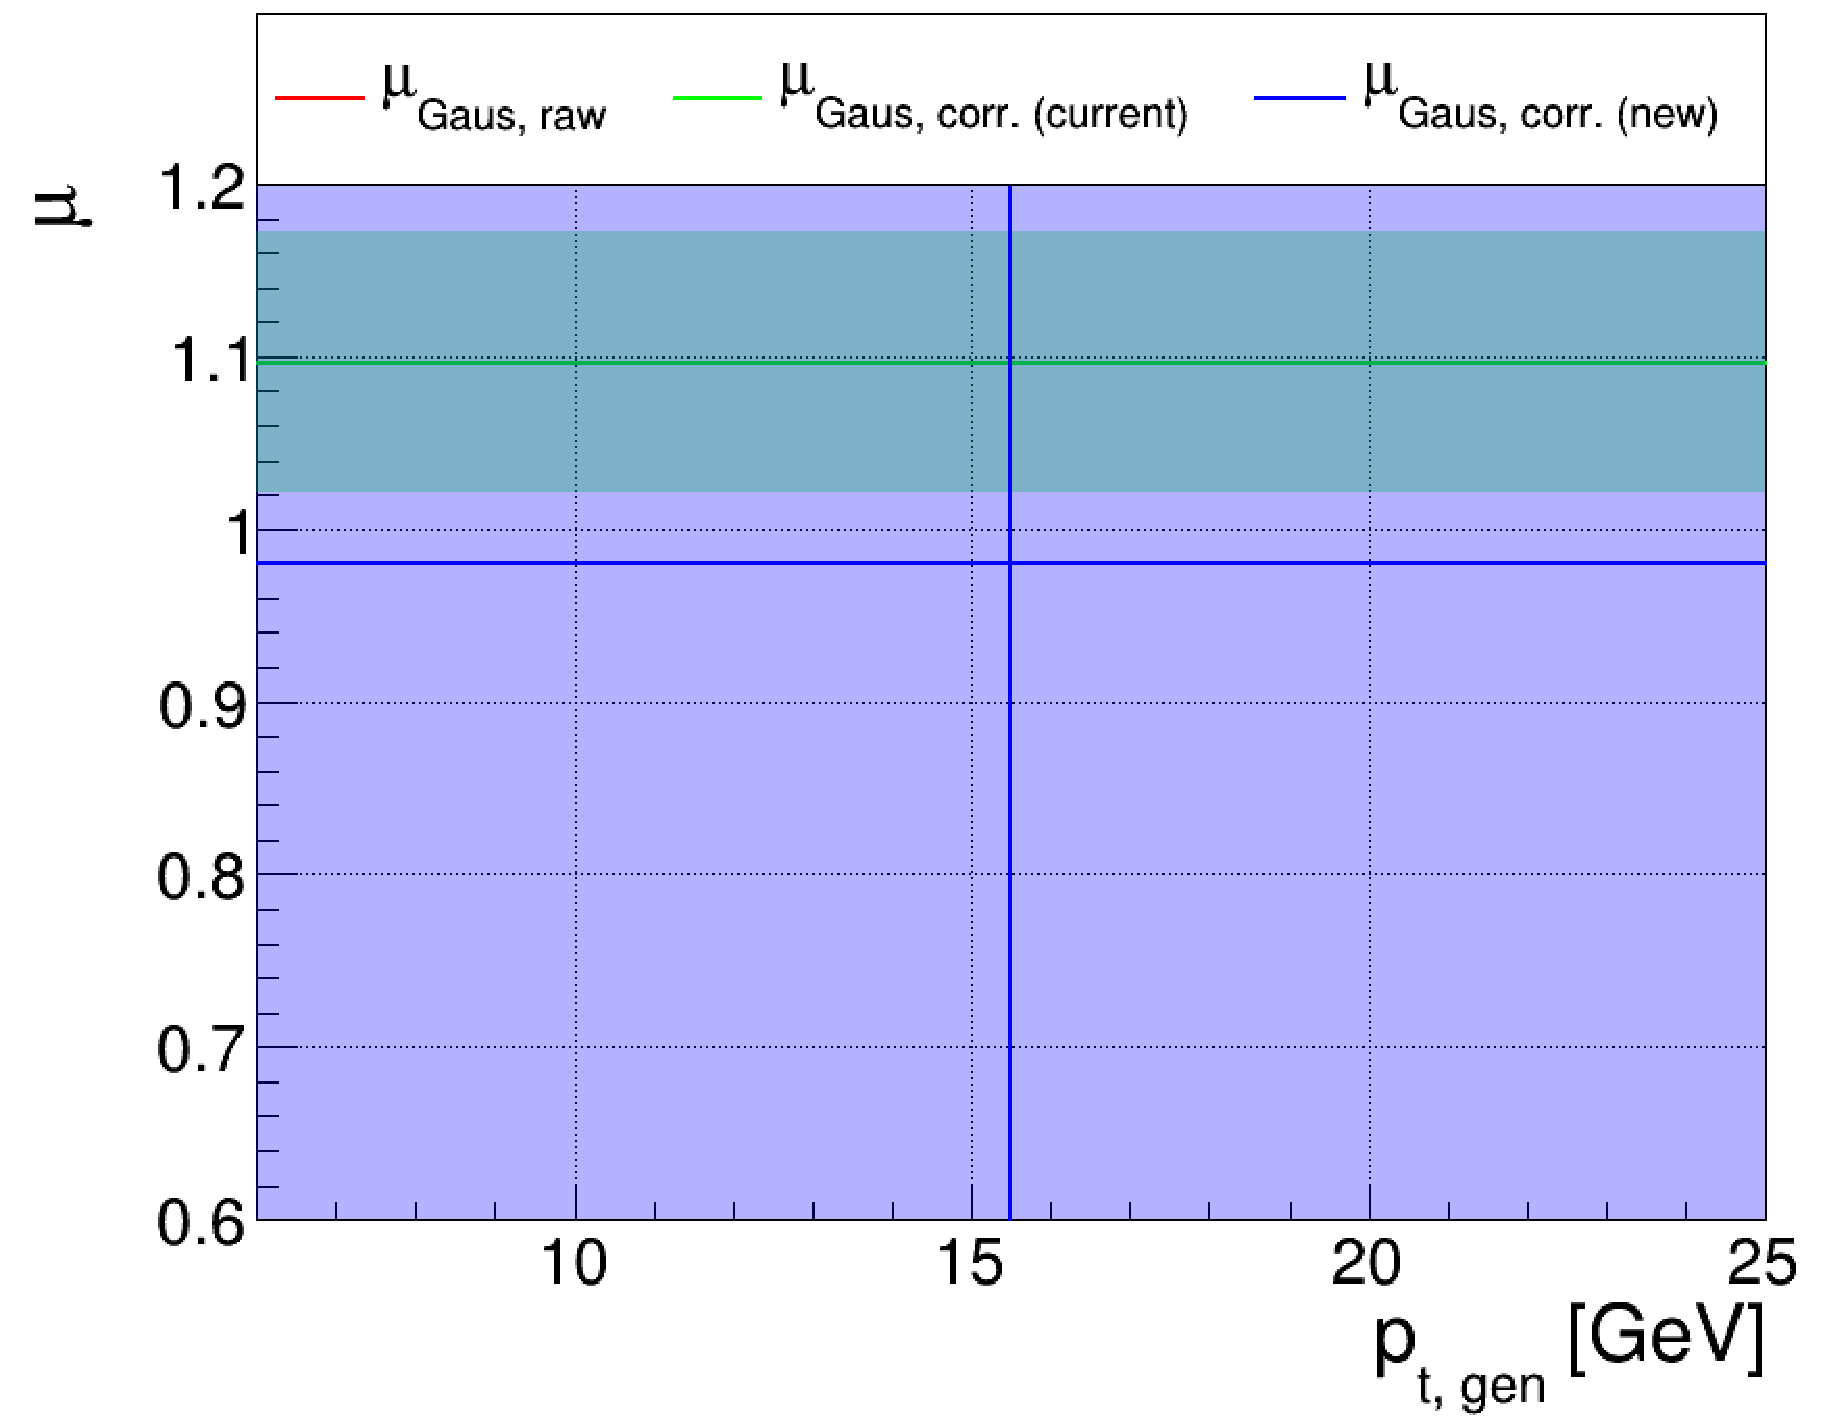
\includegraphics[width=0.495\textwidth]{./ECAL_plots/plotsNOPU/EB/ZS/pdf/GENPT/EBZS_GENPT_0006_0025_MuOverBins.pdf}
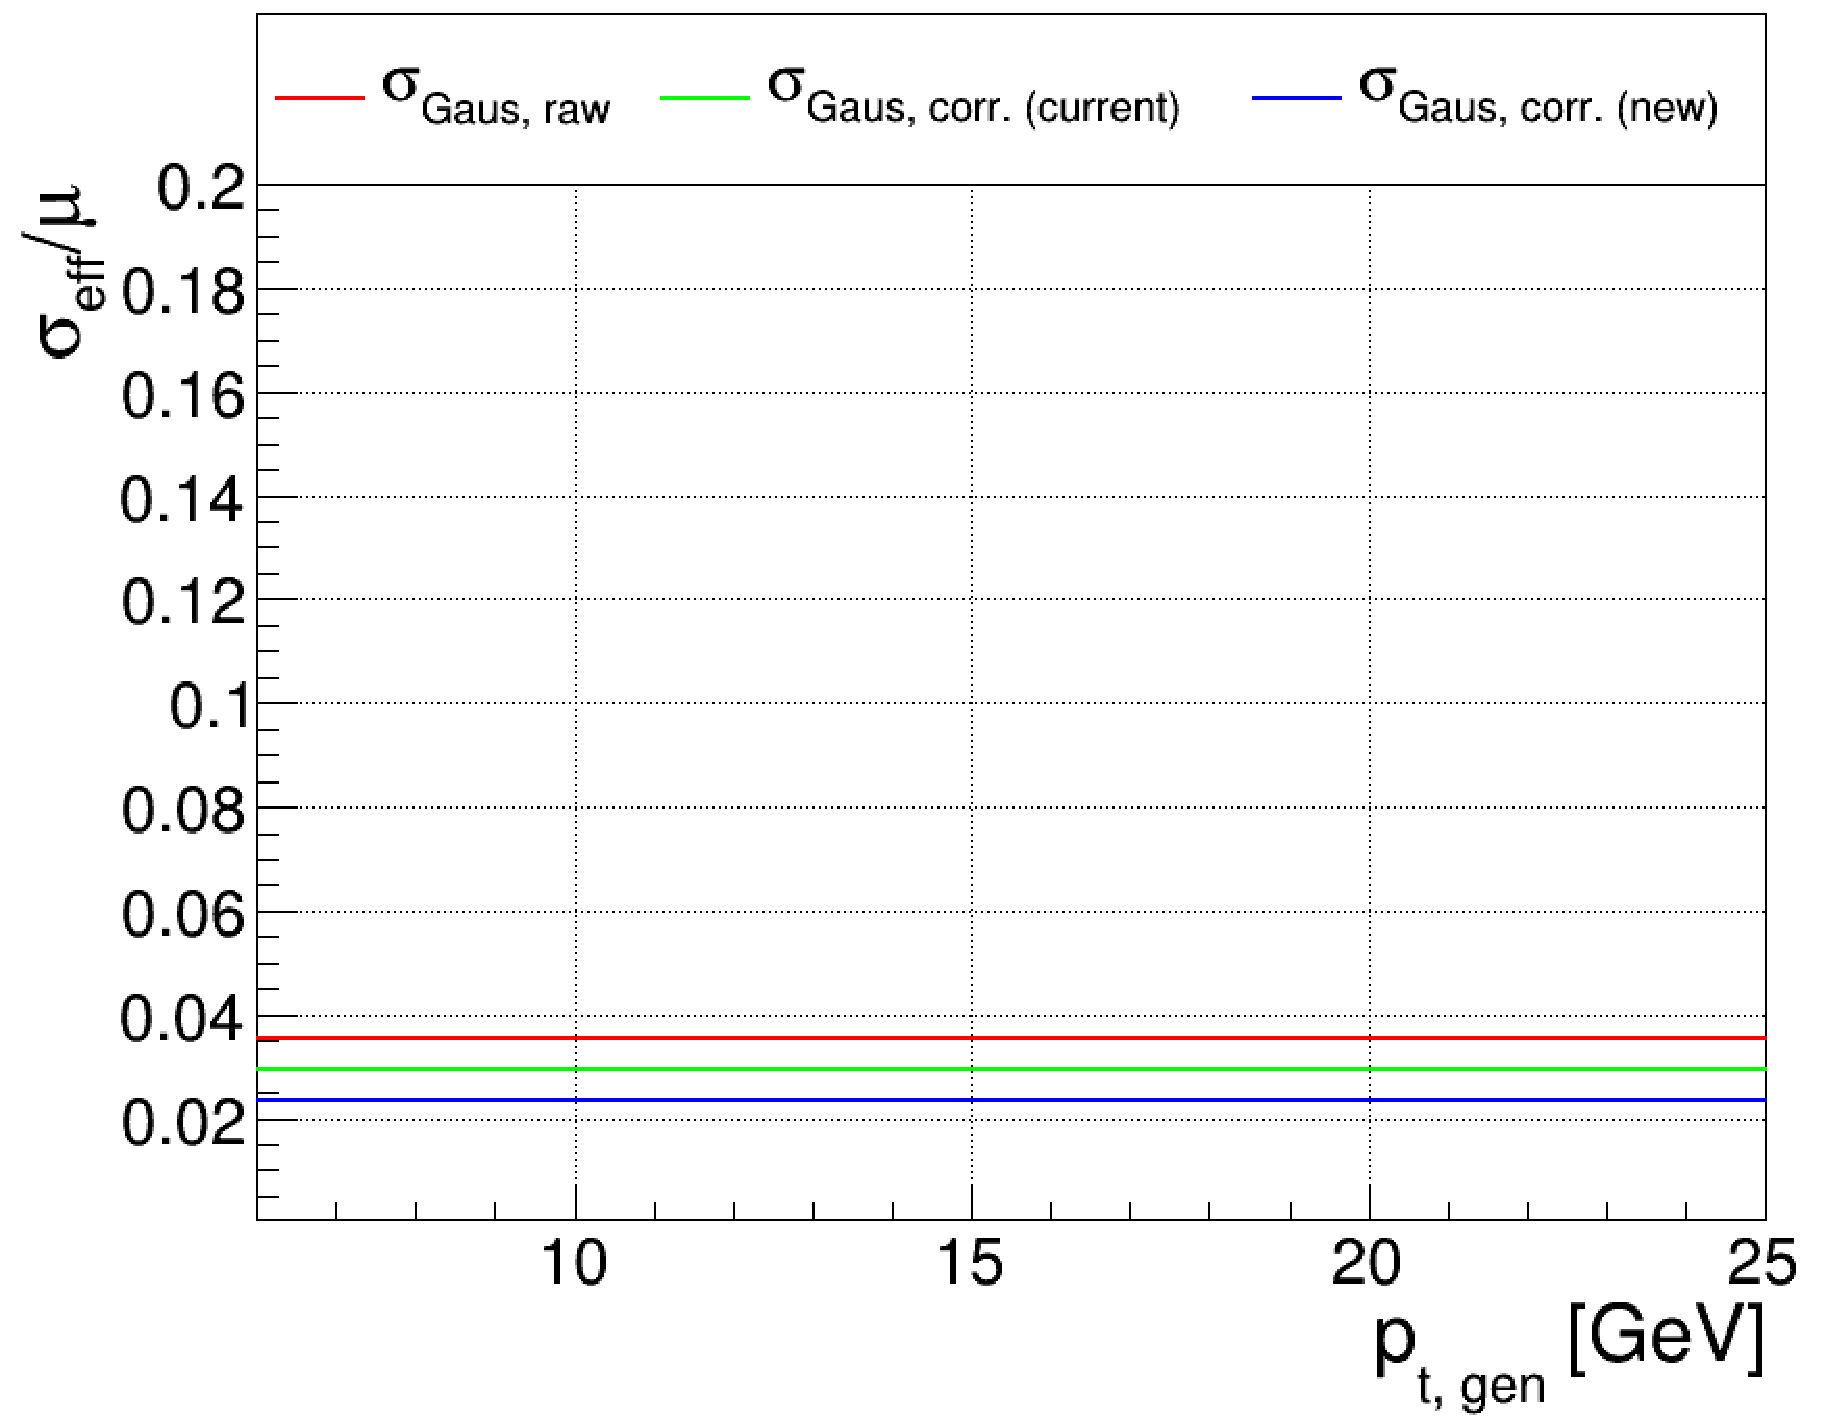
\includegraphics[width=0.495\textwidth]{./ECAL_plots/plotsNOPU/EB/ZS/pdf/GENPT/EBZS_GENPT_0006_0025_EffSigmaOverBins.pdf}
%\caption{EB - ZS Readout pt 6-25}
%\end{figure}
%\begin{figure}
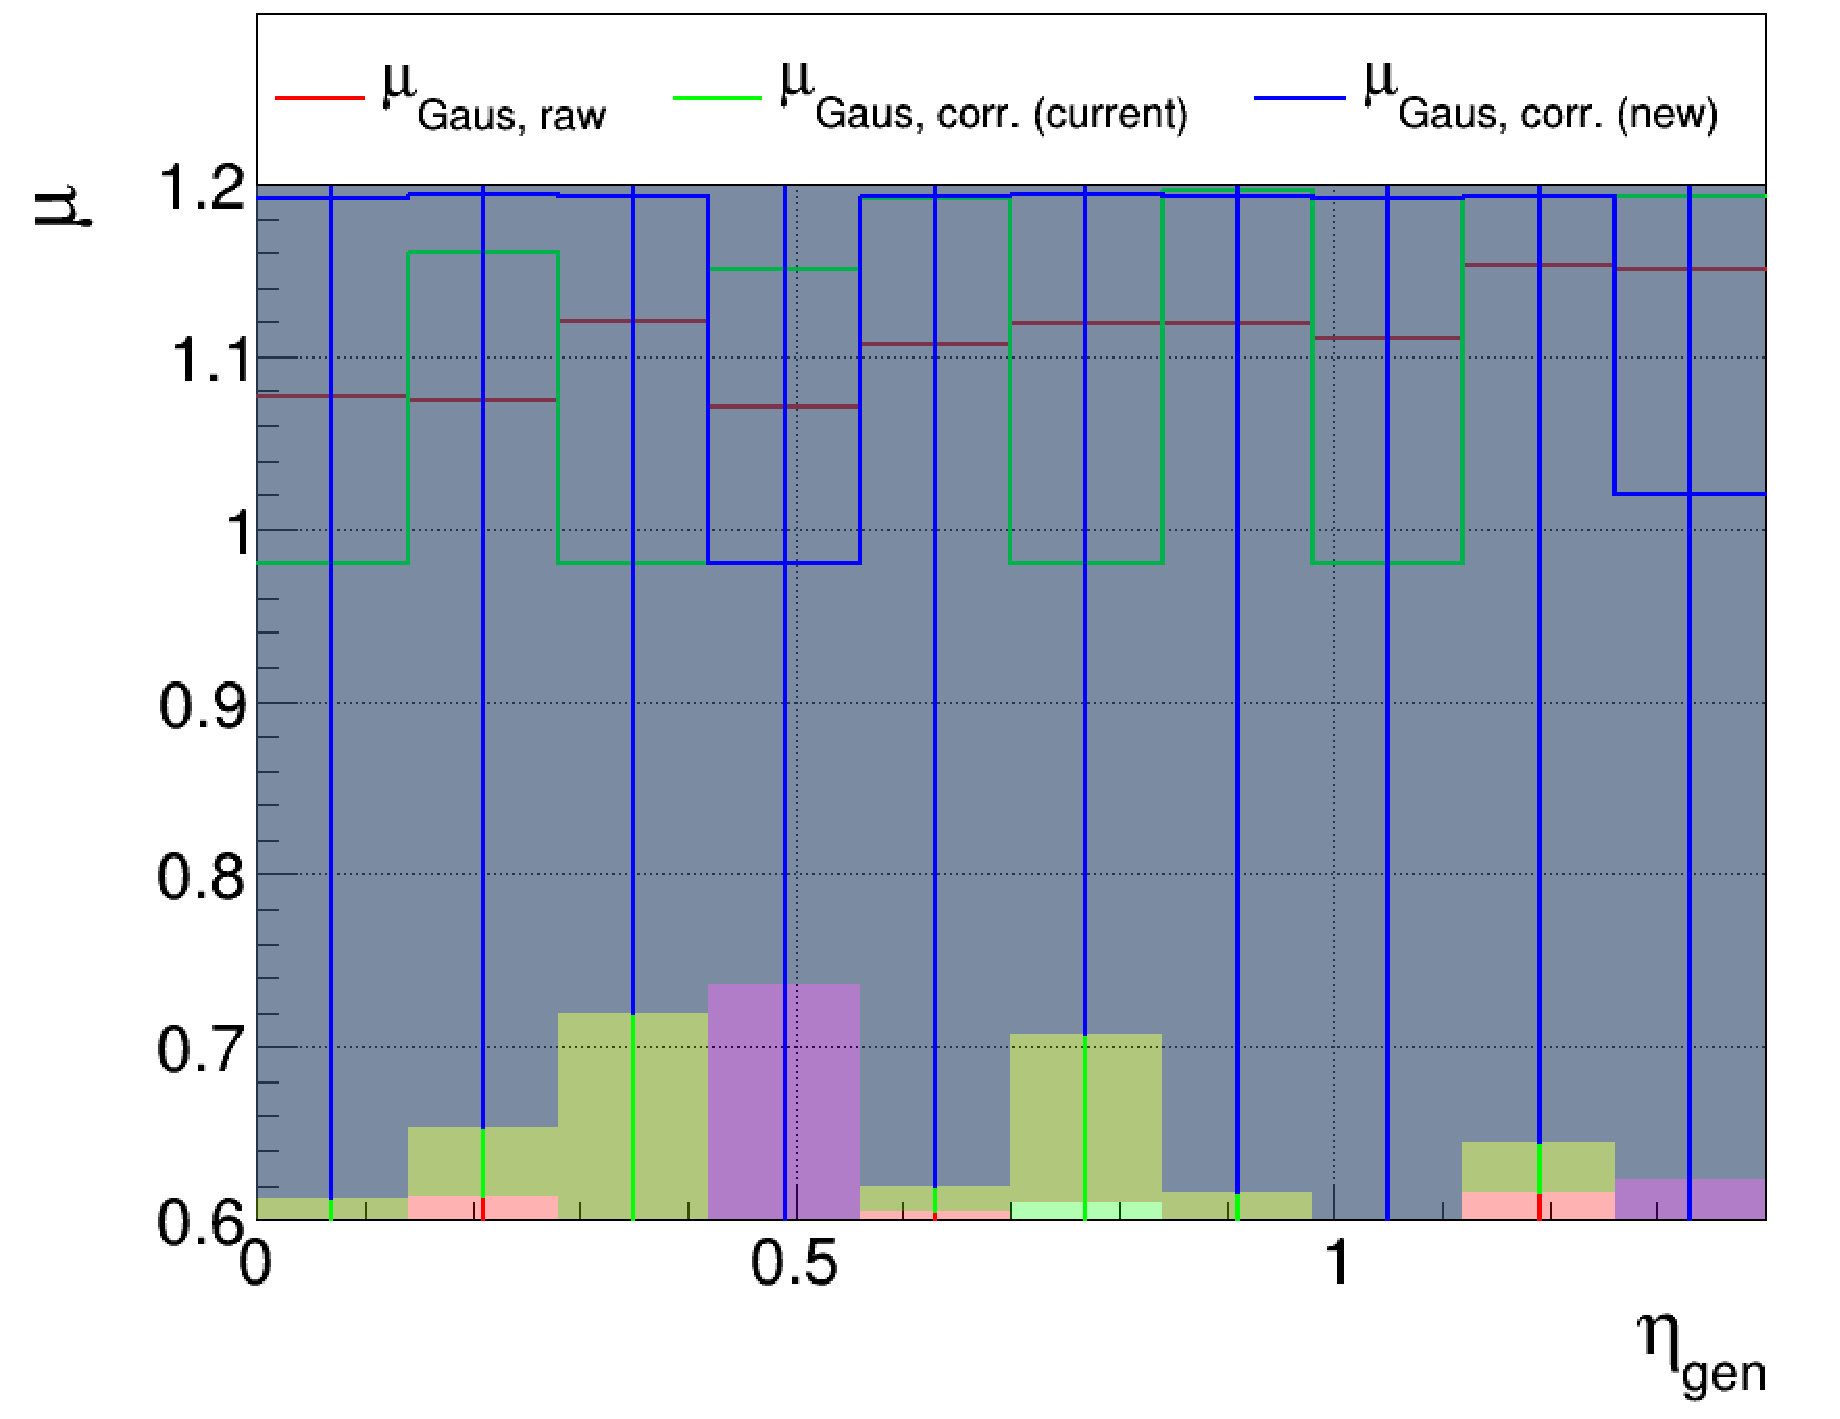
\includegraphics[width=0.495\textwidth]{./ECAL_plots/plotsNOPU/EB/ZS/pdf/GENETA/EBZS_GENETA_0006_0025_MuOverBins.pdf}
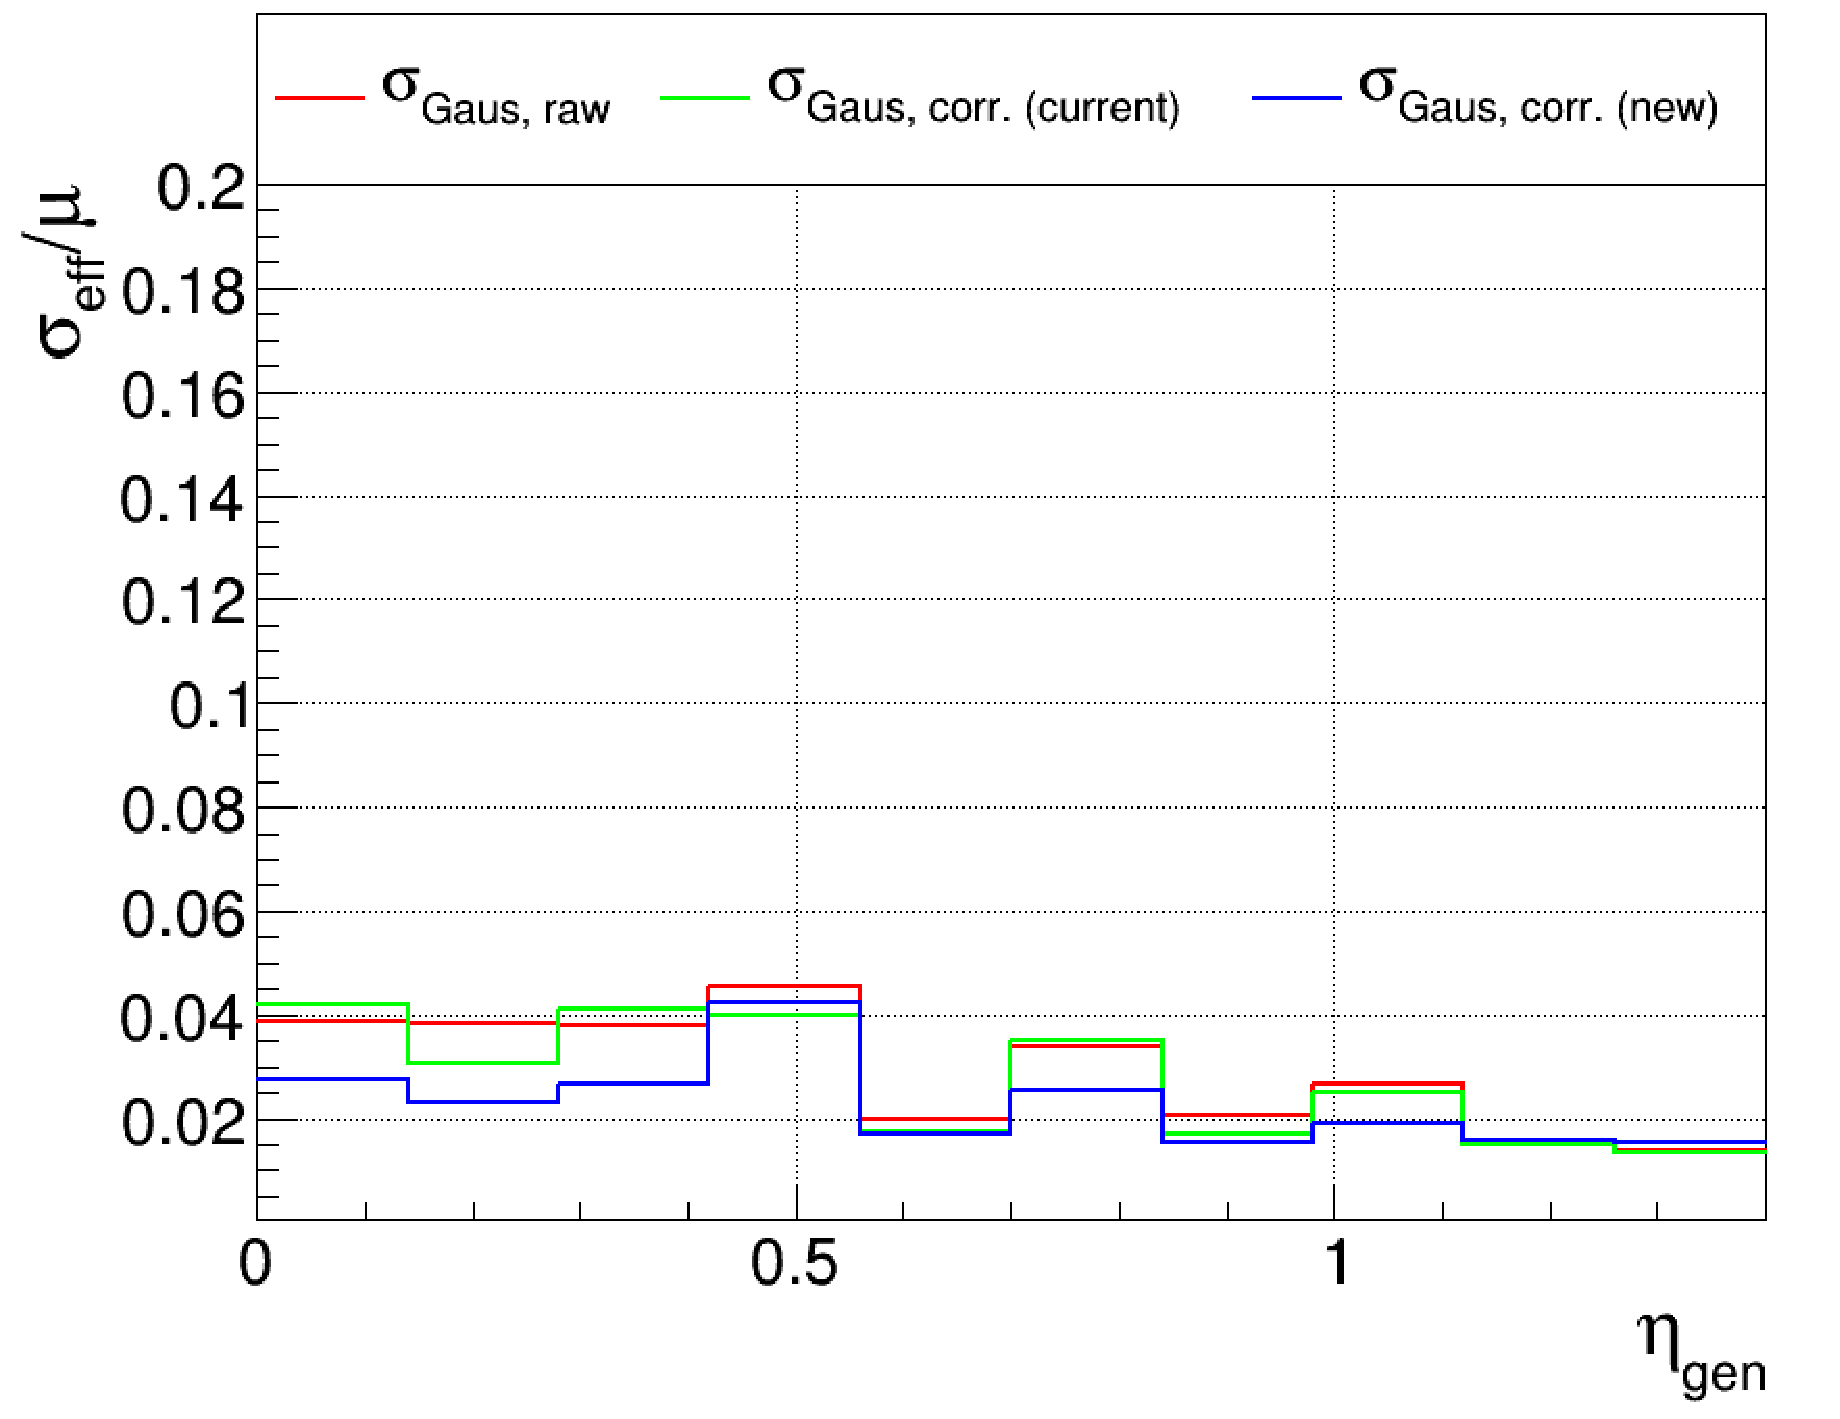
\includegraphics[width=0.495\textwidth]{./ECAL_plots/plotsNOPU/EB/ZS/pdf/GENETA/EBZS_GENETA_0006_0025_EffSigmaOverBins.pdf}
\caption{EB - ZS Readout pt 6-25}
\end{figure}





\begin{figure}
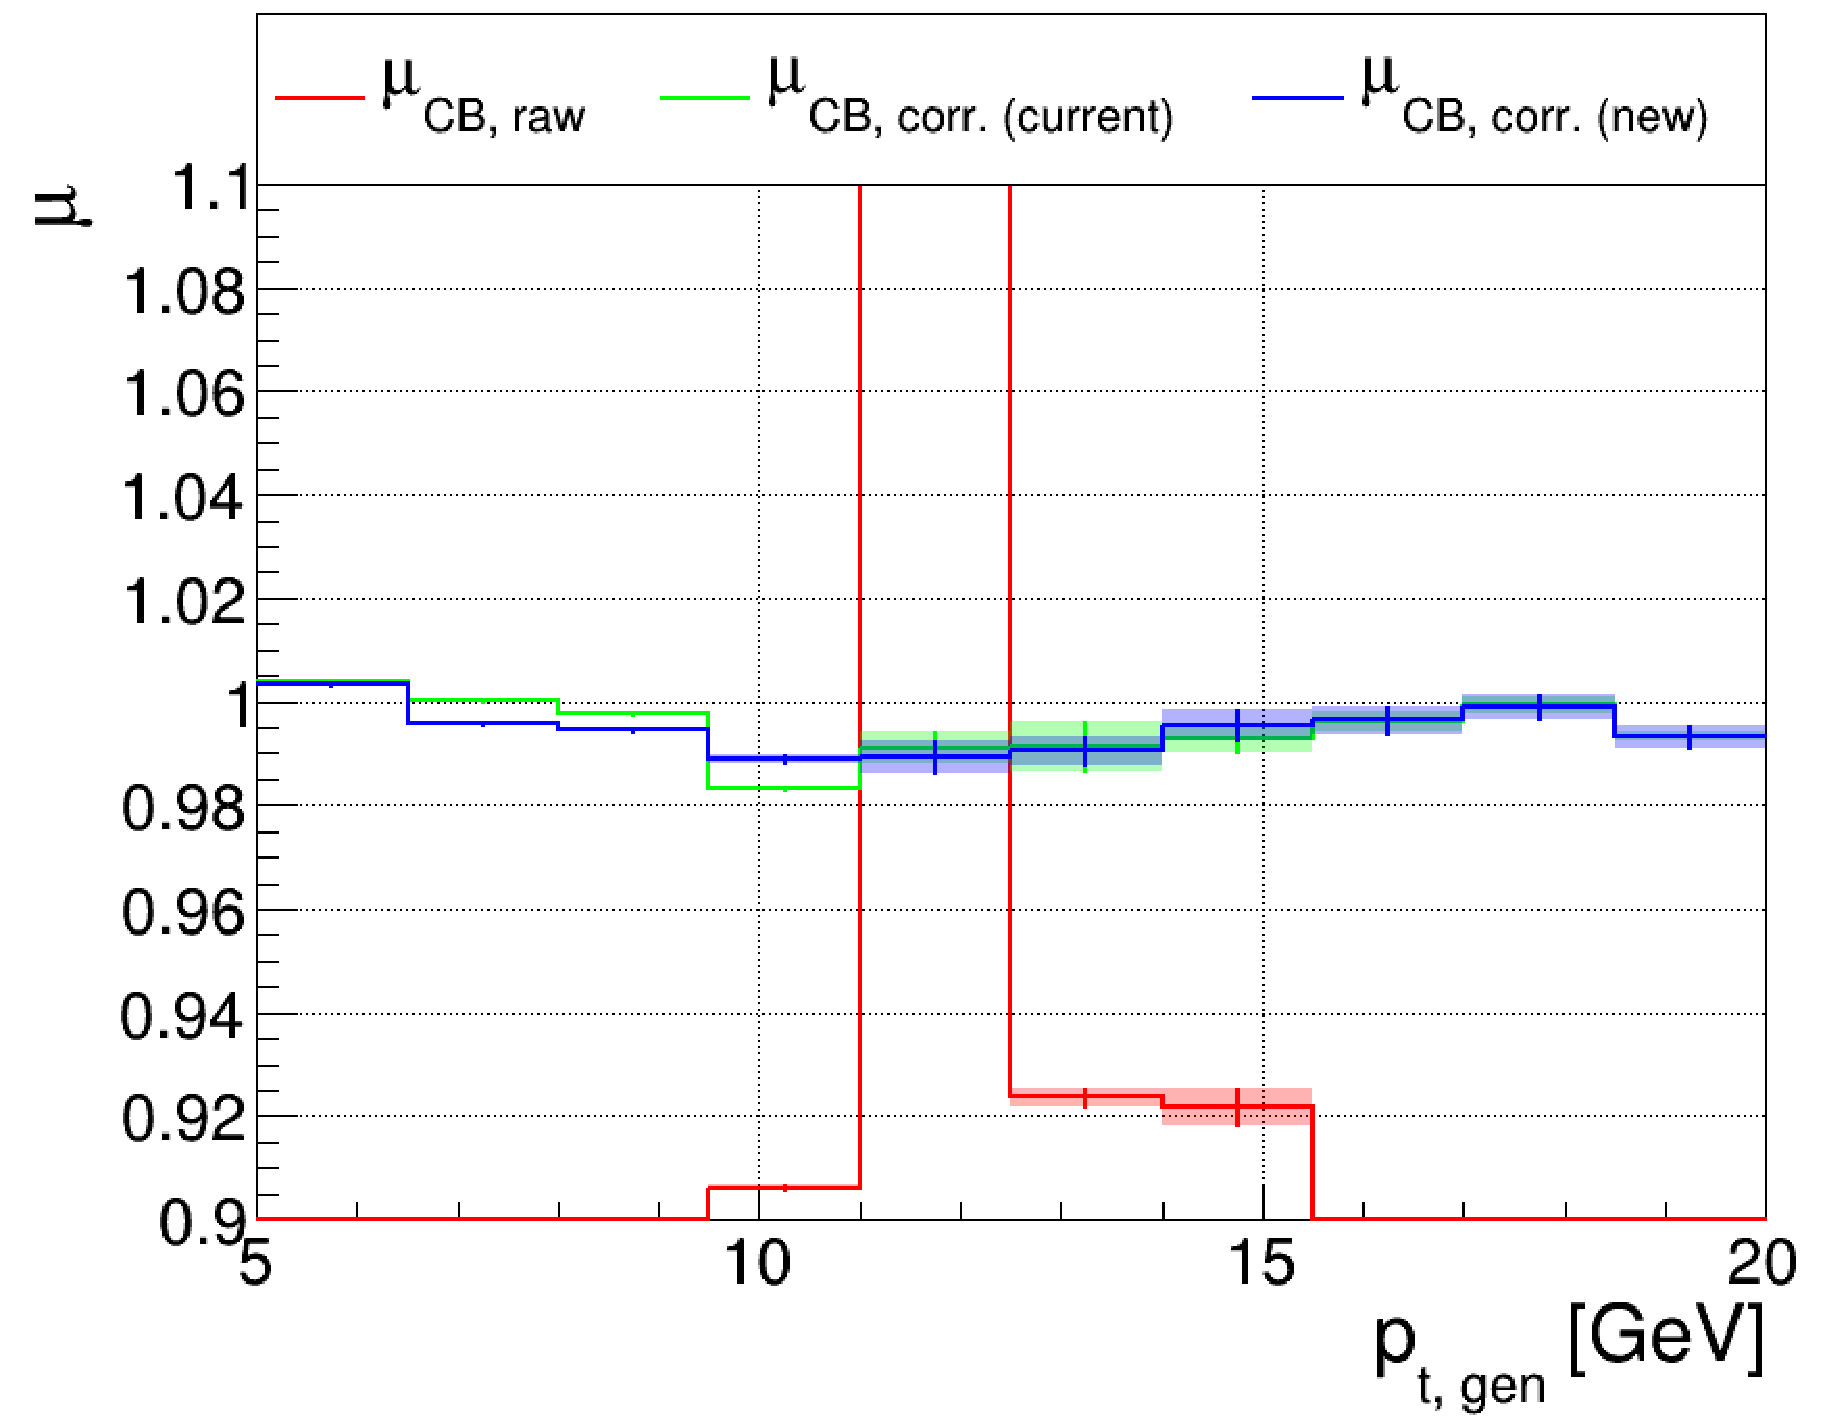
\includegraphics[width=0.495\textwidth]{./ECAL_plots/plotsNoPU/EE/pdf/FULL/GENPT/EEFULL_GENPT_0005_0020_MuOverBins.pdf}
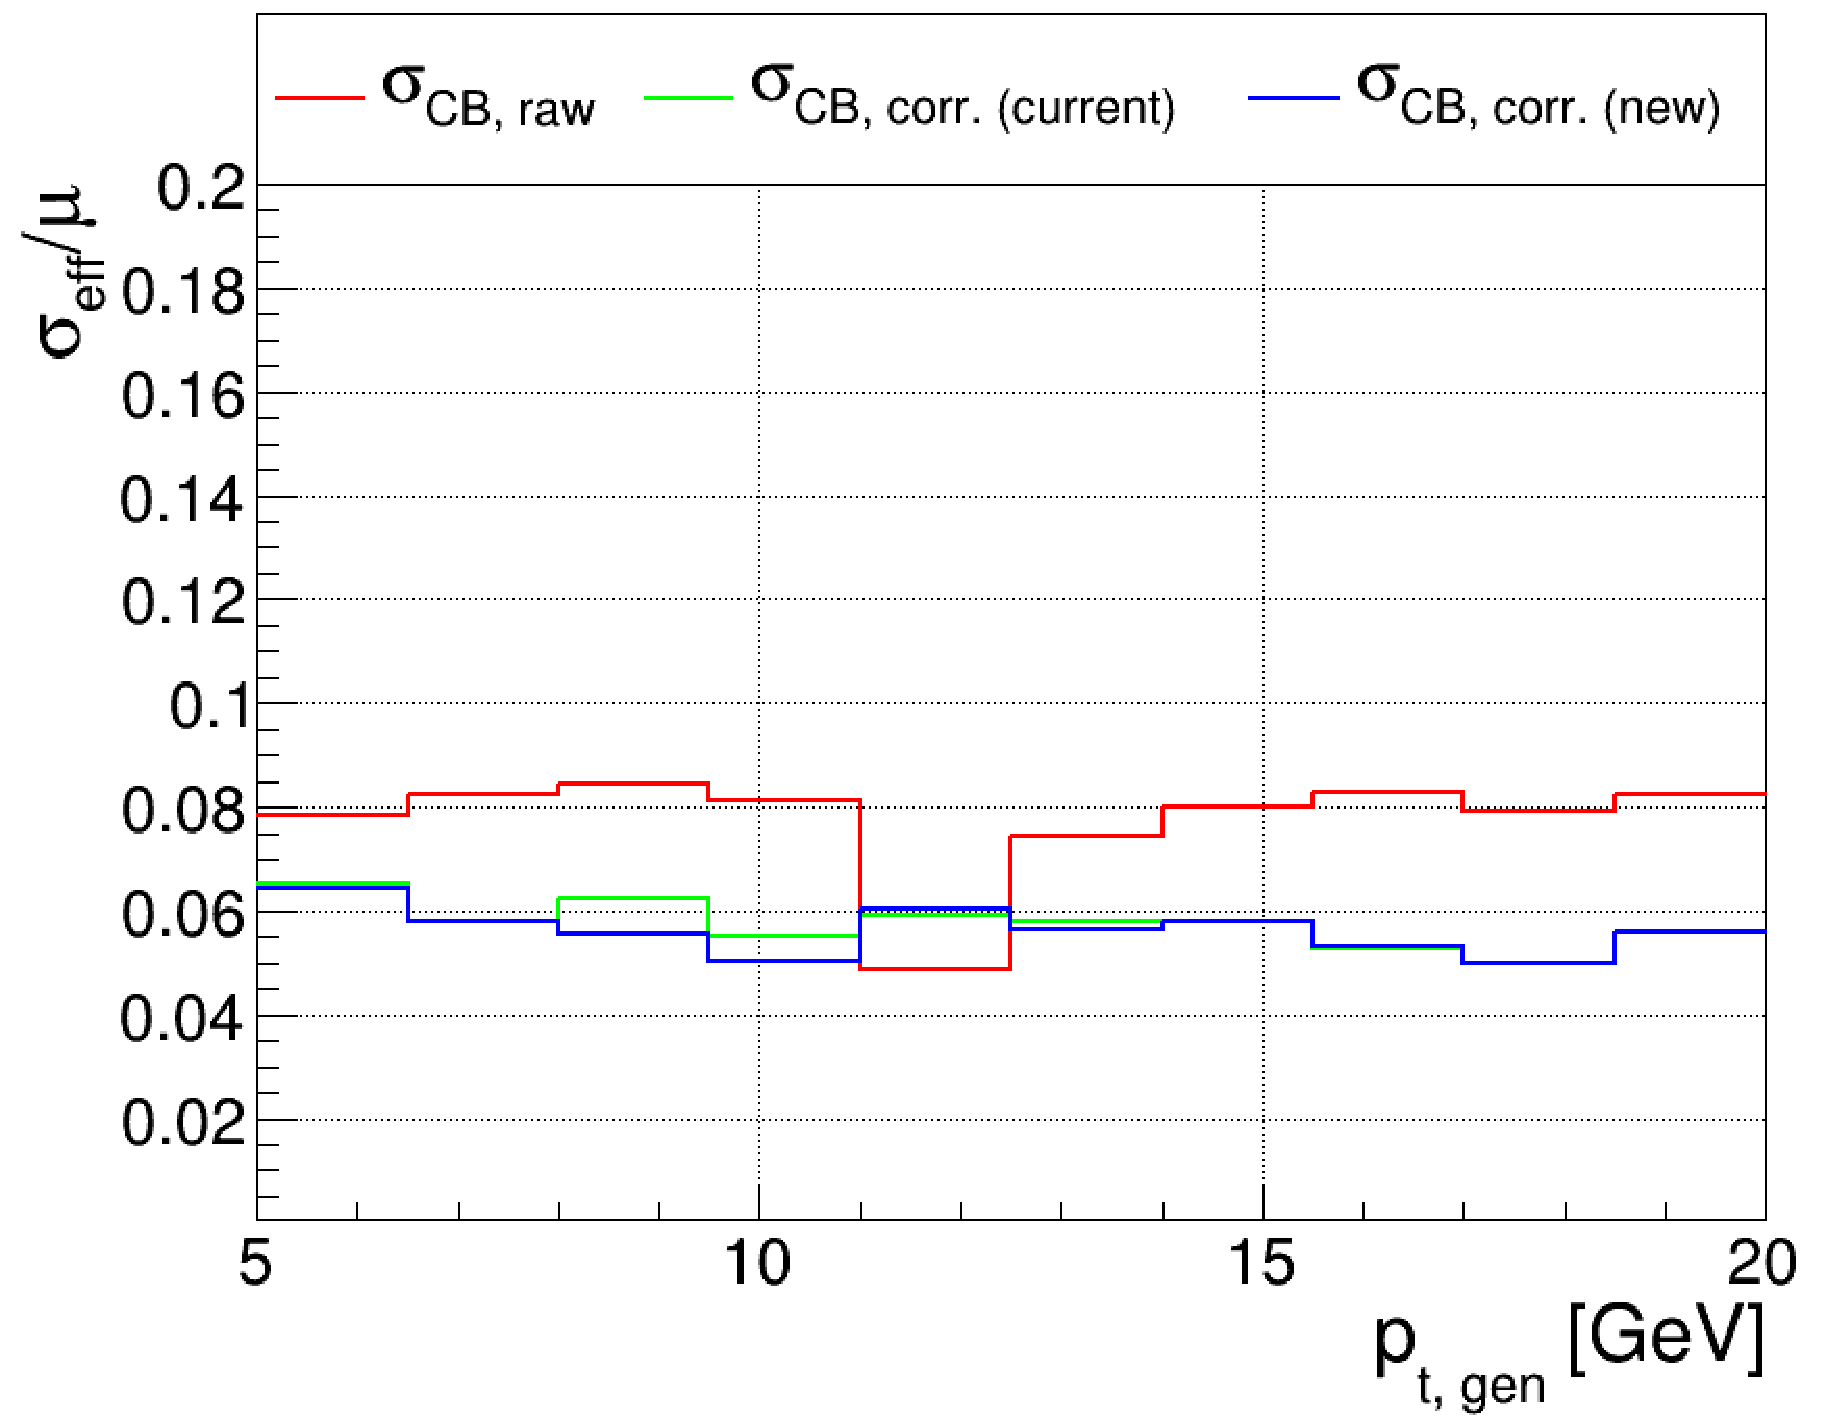
\includegraphics[width=0.495\textwidth]{./ECAL_plots/plotsNoPU/EE/pdf/FULL/GENPT/EEFULL_GENPT_0005_0020_EffSigmaOverBins.pdf}
%\caption{EE - Full Readout pt 5-20}
%\end{figure}
%\begin{figure}
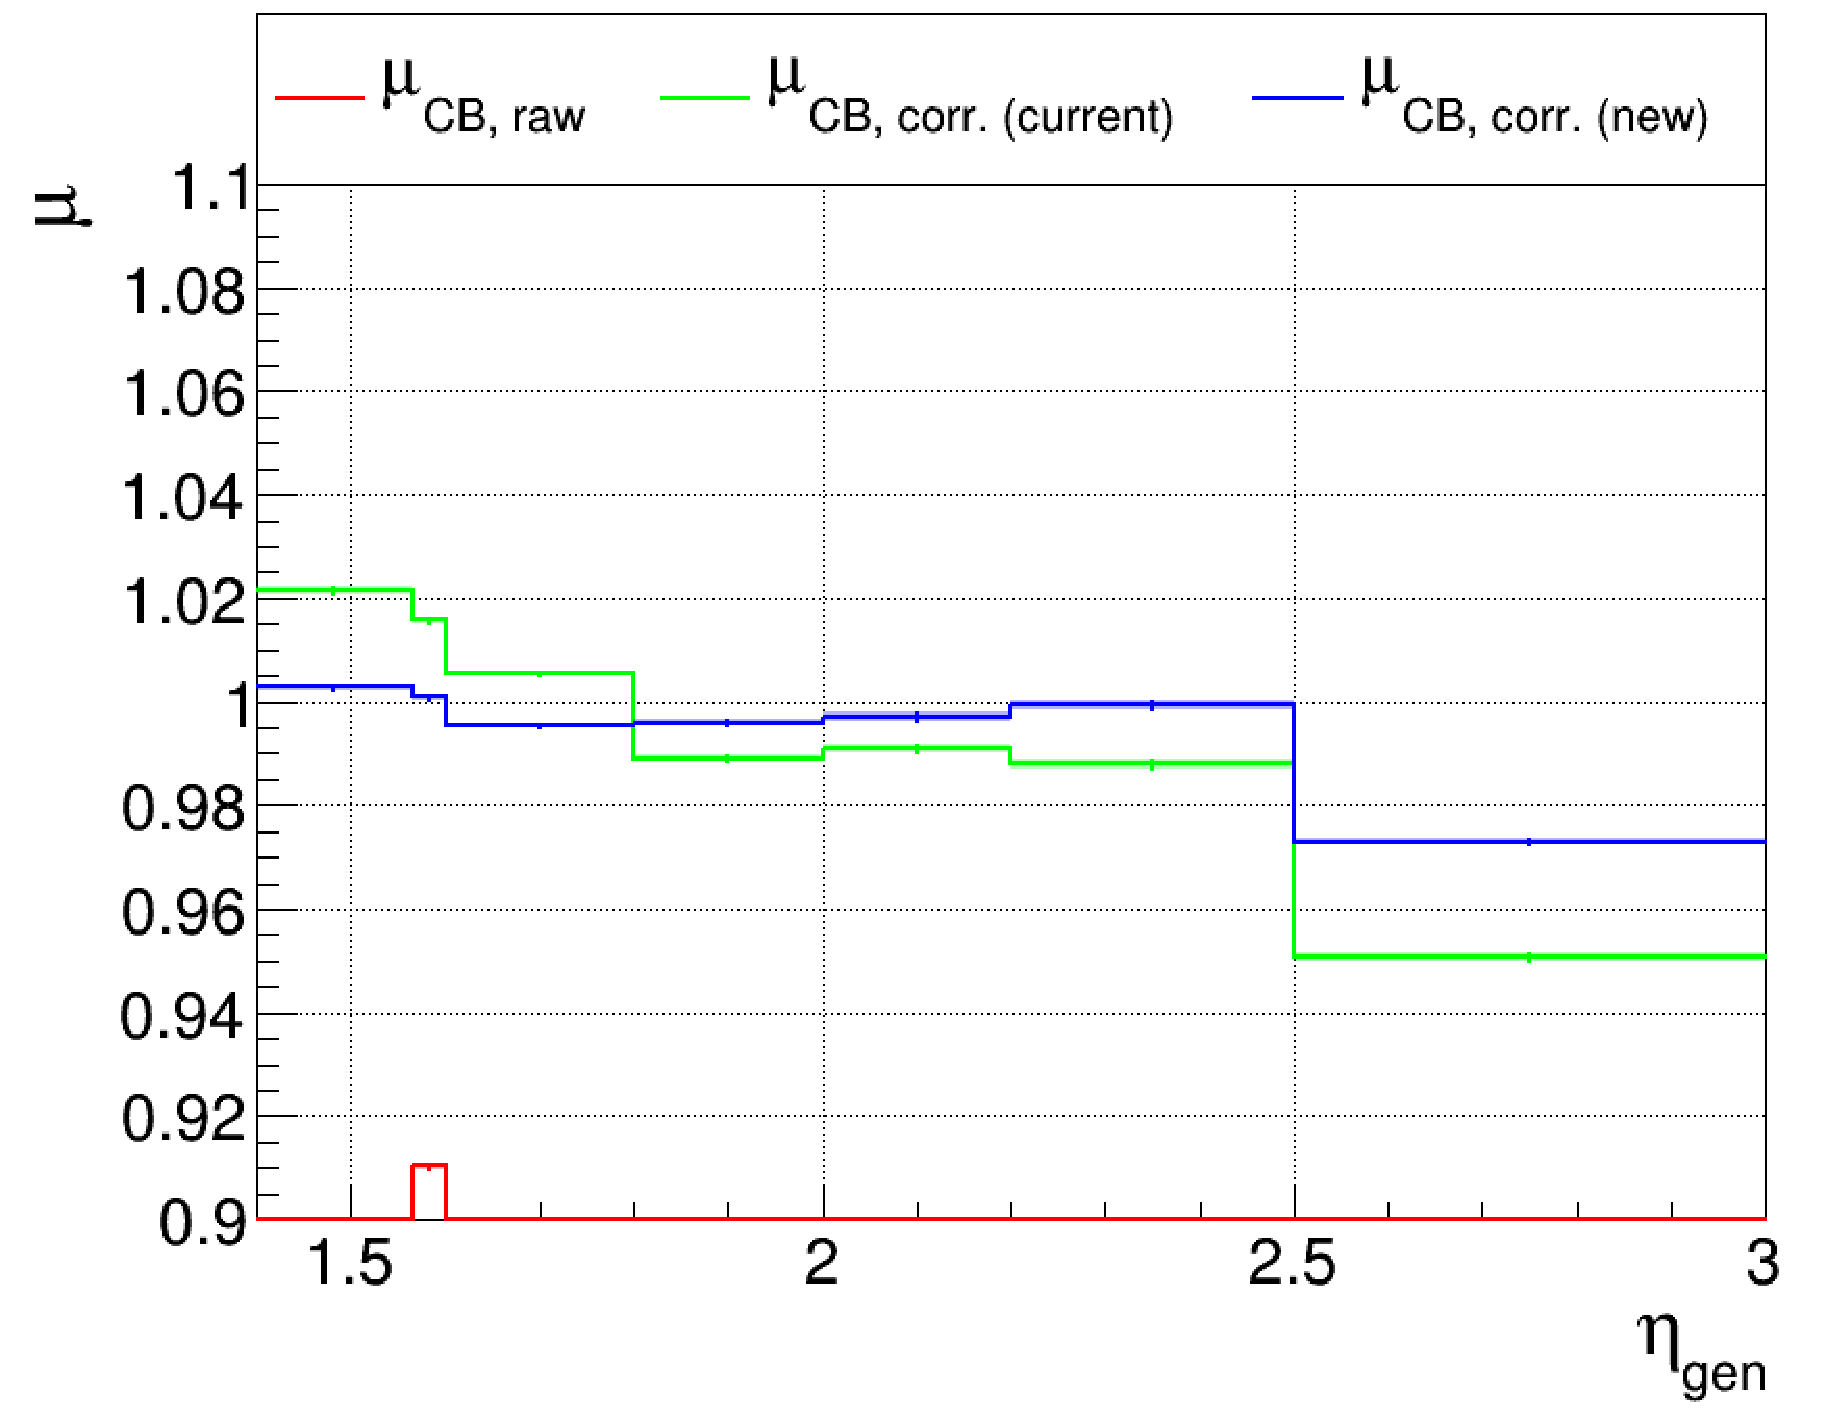
\includegraphics[width=0.495\textwidth]{./ECAL_plots/plotsNoPU/EE/pdf/FULL/GENETA/EEFULL_GENETA_0005_0020_MuOverBins.pdf}
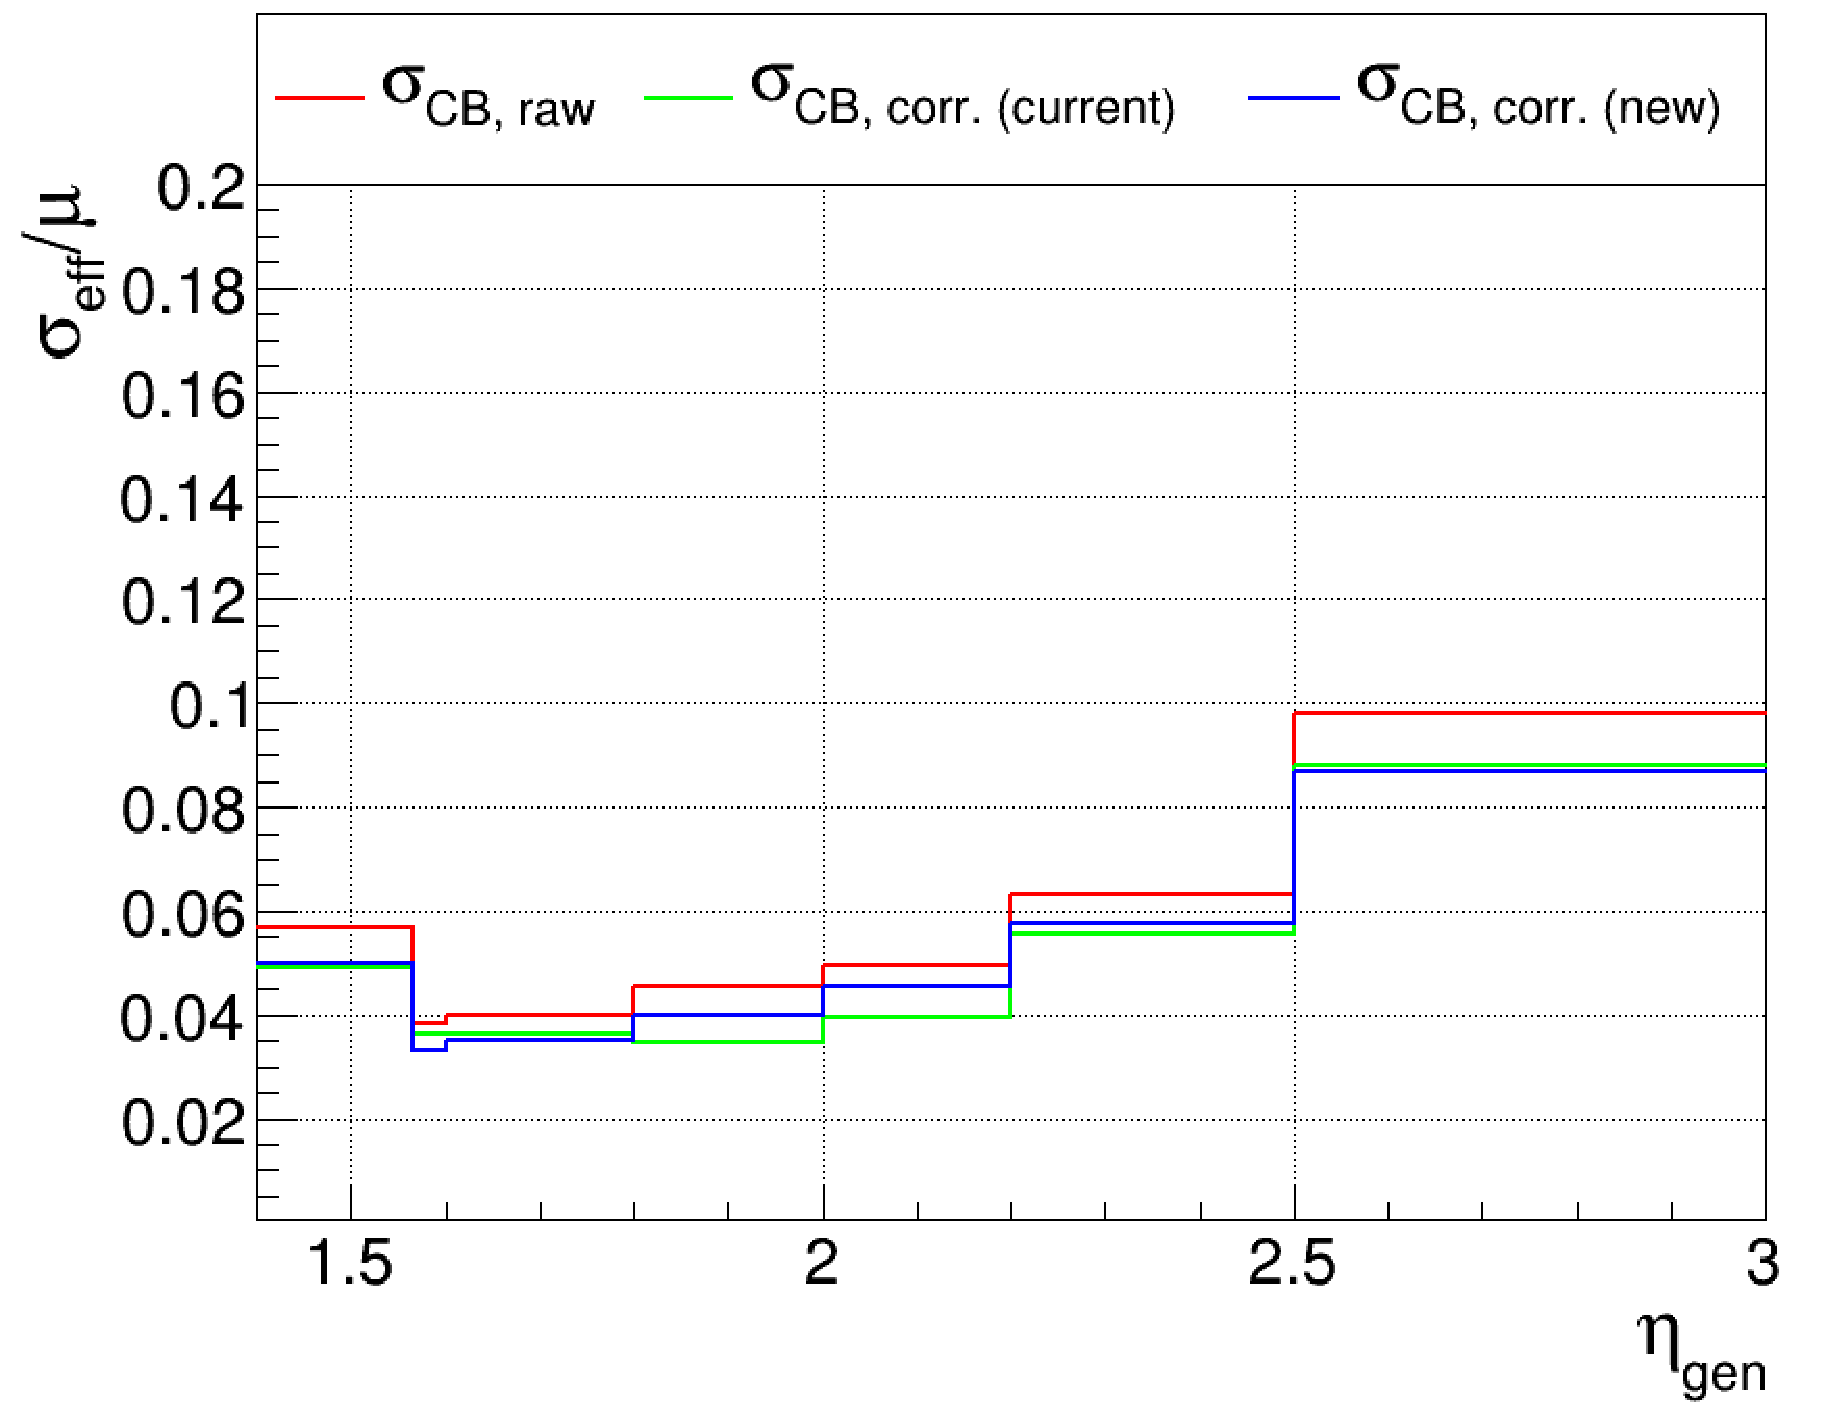
\includegraphics[width=0.495\textwidth]{./ECAL_plots/plotsNoPU/EE/pdf/FULL/GENETA/EEFULL_GENETA_0005_0020_EffSigmaOverBins.pdf}
\caption{EE - Full Readout pt 5-20}
\end{figure}


\begin{figure}
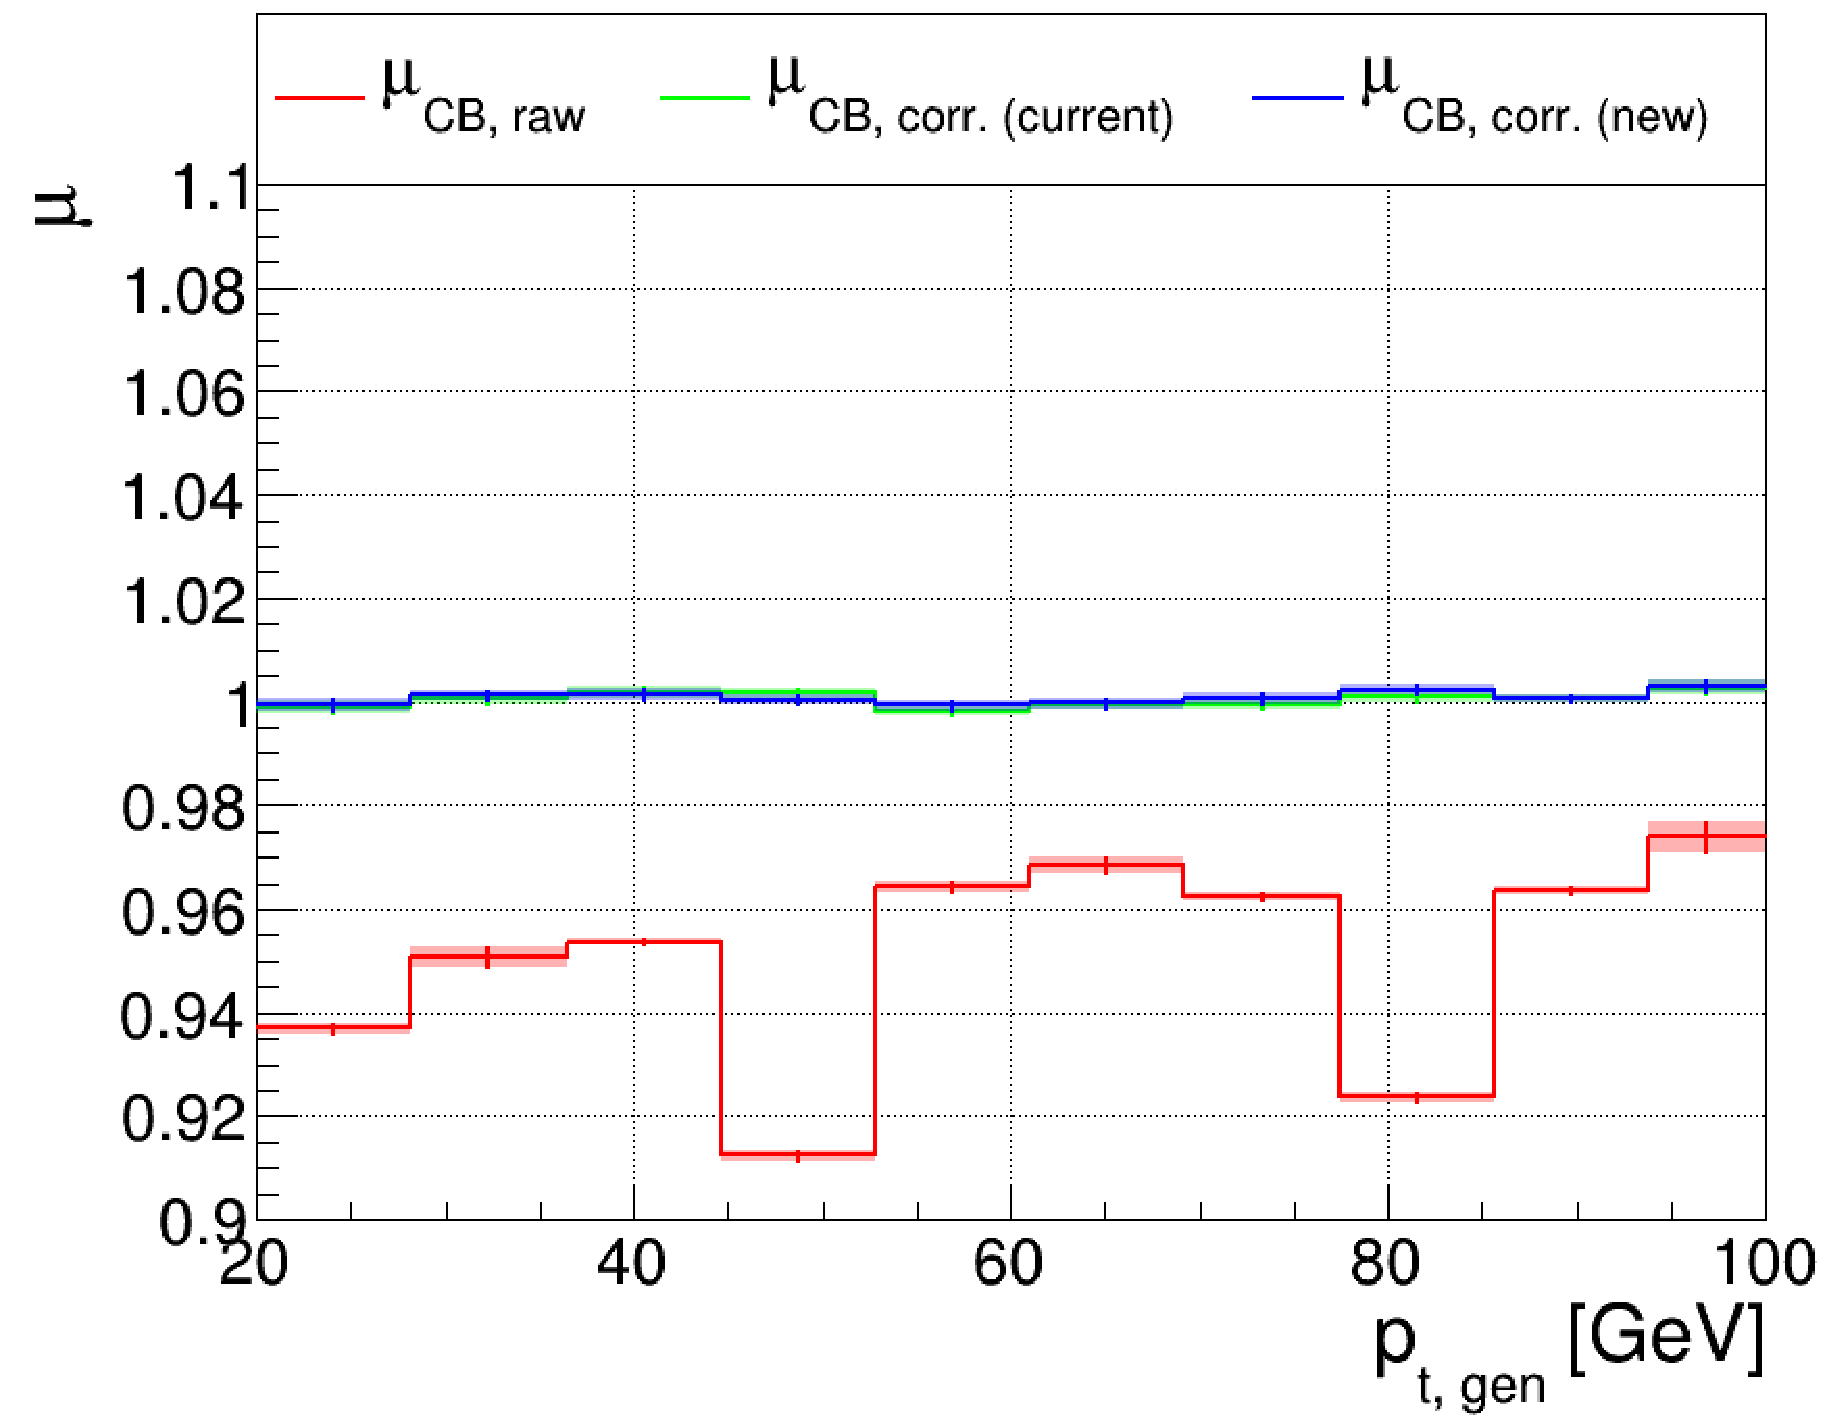
\includegraphics[width=0.495\textwidth]{./ECAL_plots/plotsNoPU/EE/pdf/FULL/GENPT/EEFULL_GENPT_0020_0100_MuOverBins.pdf}
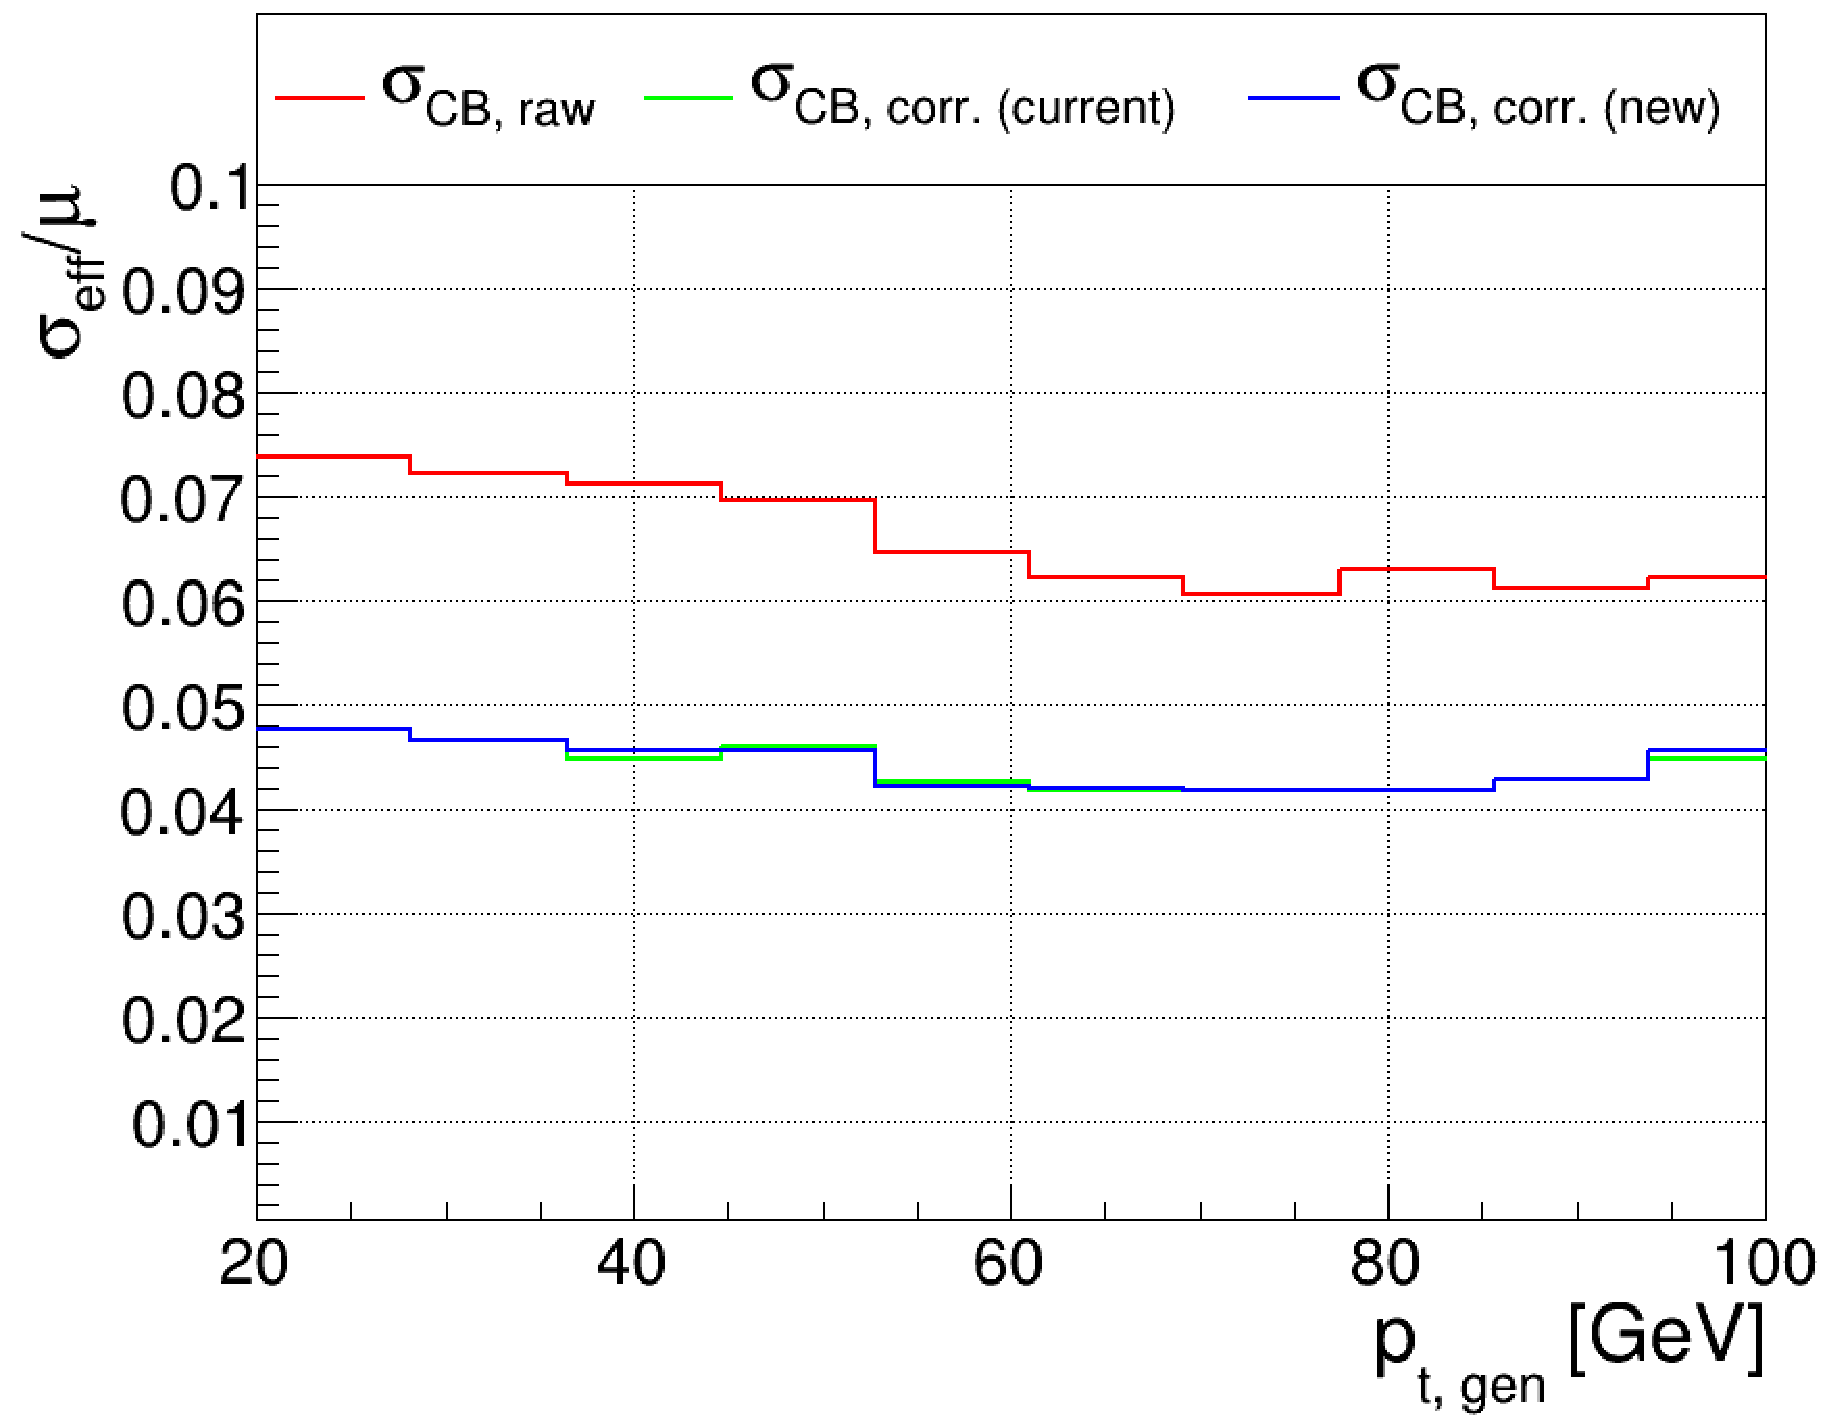
\includegraphics[width=0.495\textwidth]{./ECAL_plots/plotsNoPU/EE/pdf/FULL/GENPT/EEFULL_GENPT_0020_0100_EffSigmaOverBins.pdf}
%\caption{EE - Full Readout pt 20-100}
%\end{figure}
%\begin{figure}
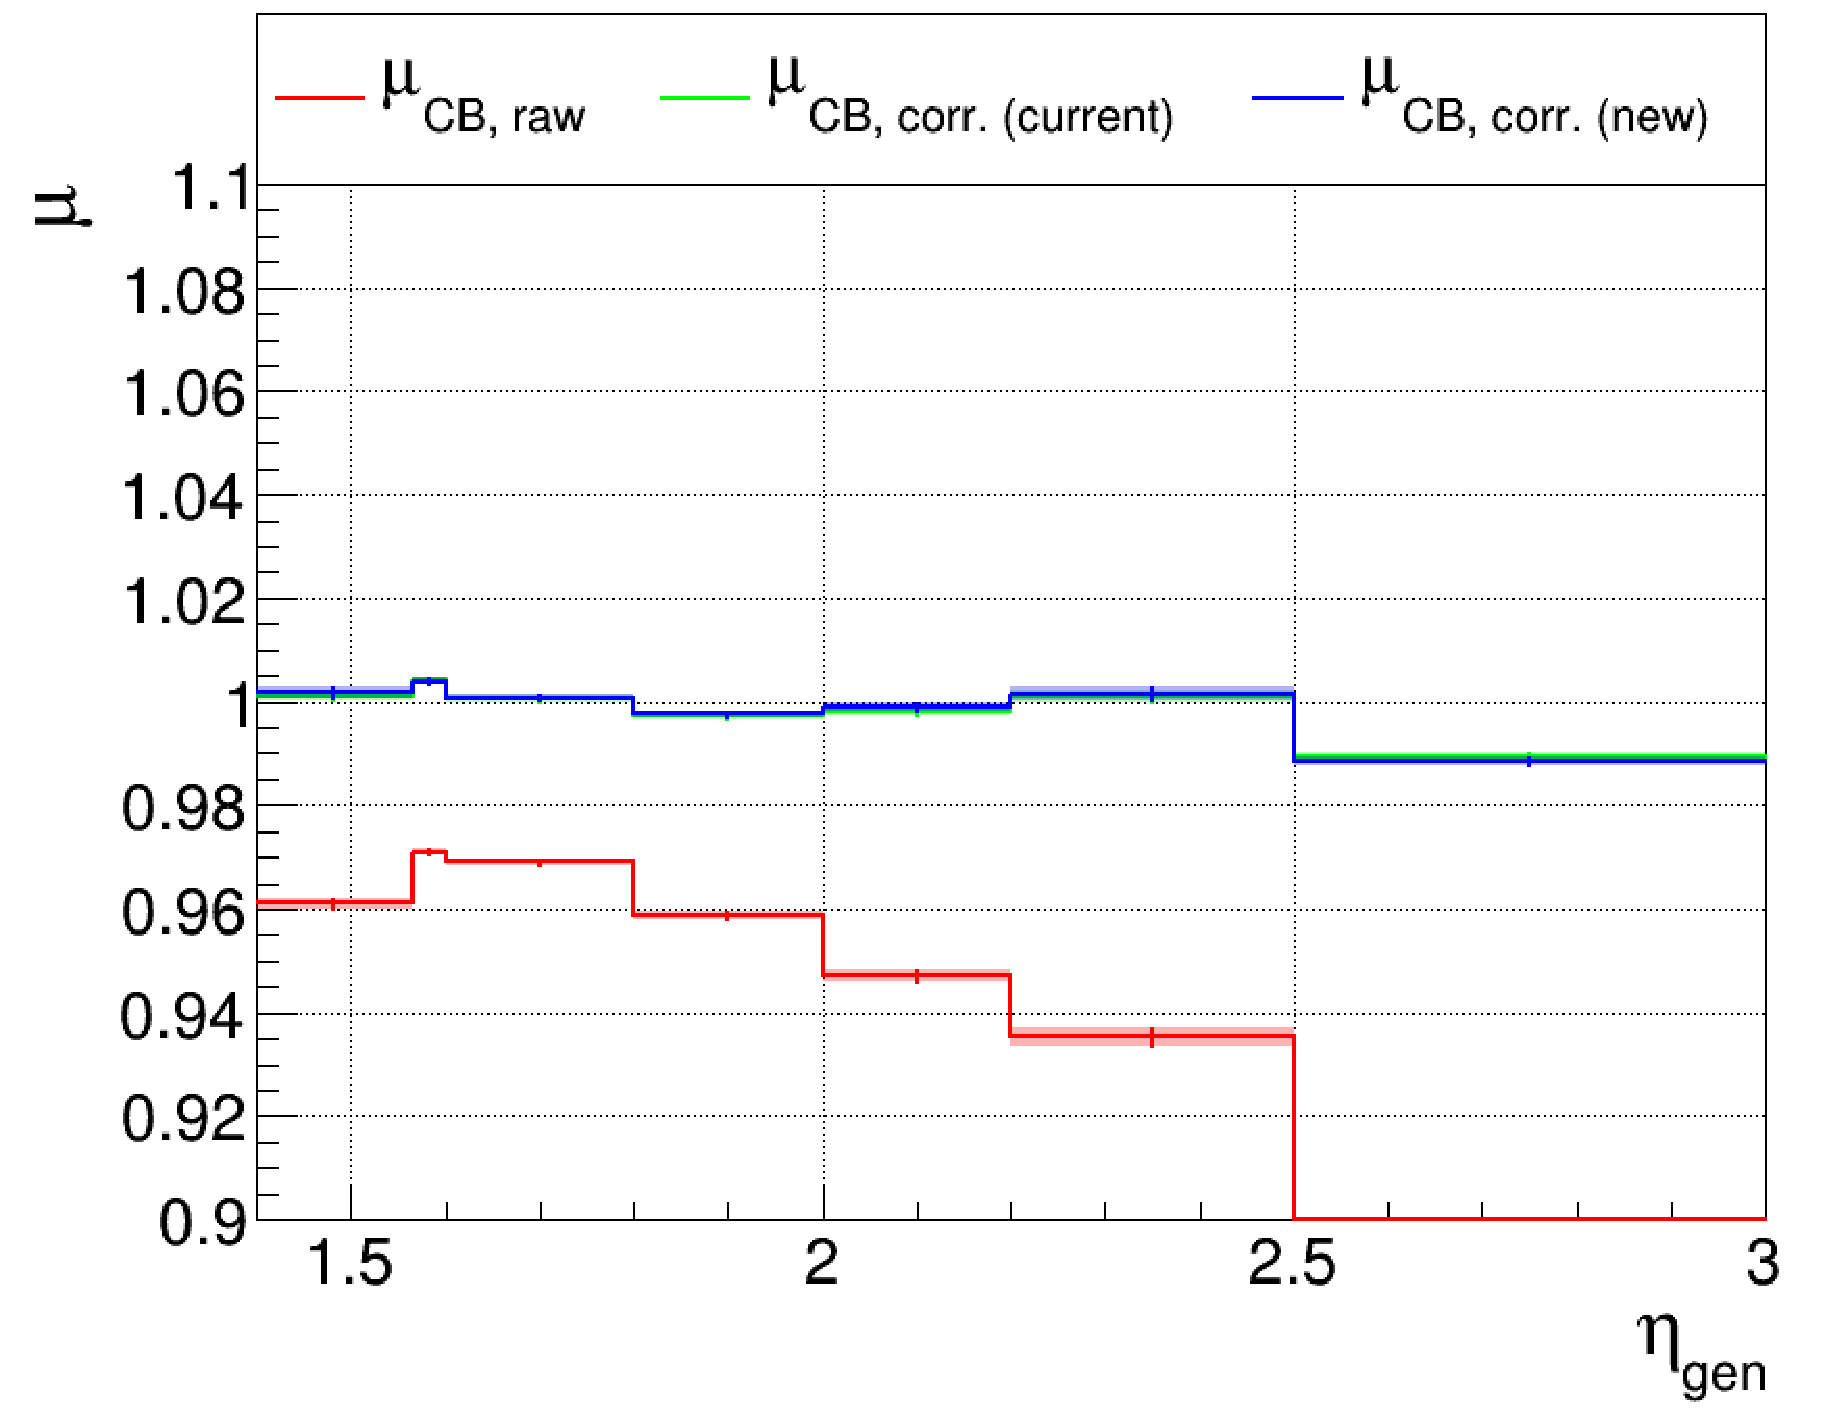
\includegraphics[width=0.495\textwidth]{./ECAL_plots/plotsNoPU/EE/pdf/FULL/GENETA/EEFULL_GENETA_0020_0100_MuOverBins.pdf}
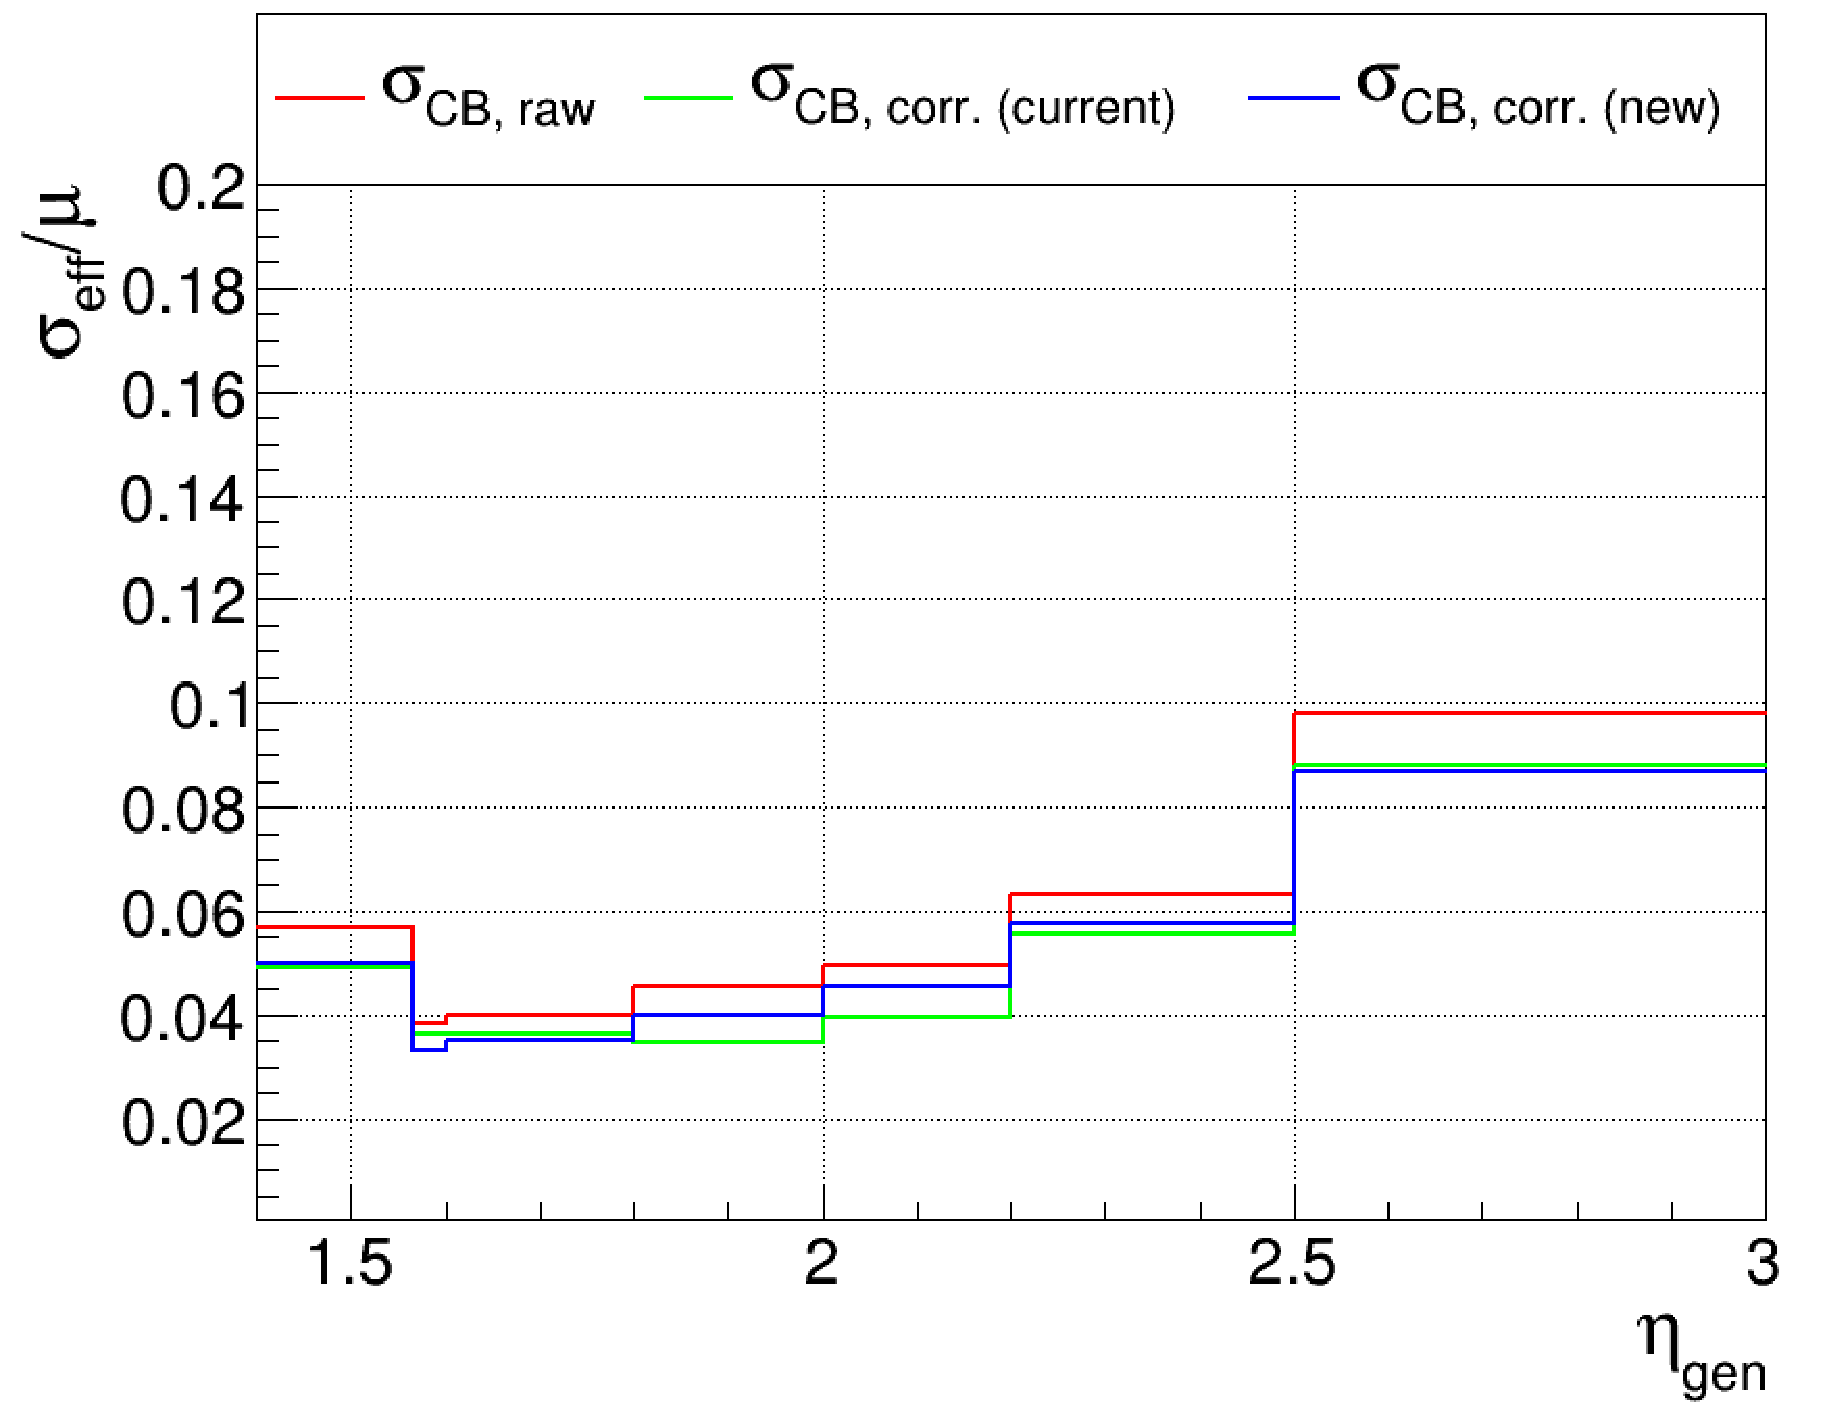
\includegraphics[width=0.495\textwidth]{./ECAL_plots/plotsNoPU/EE/pdf/FULL/GENETA/EEFULL_GENETA_0005_0020_EffSigmaOverBins.pdf}
\caption{EE - Full Readout pt 20-100}
\end{figure}


\begin{figure}
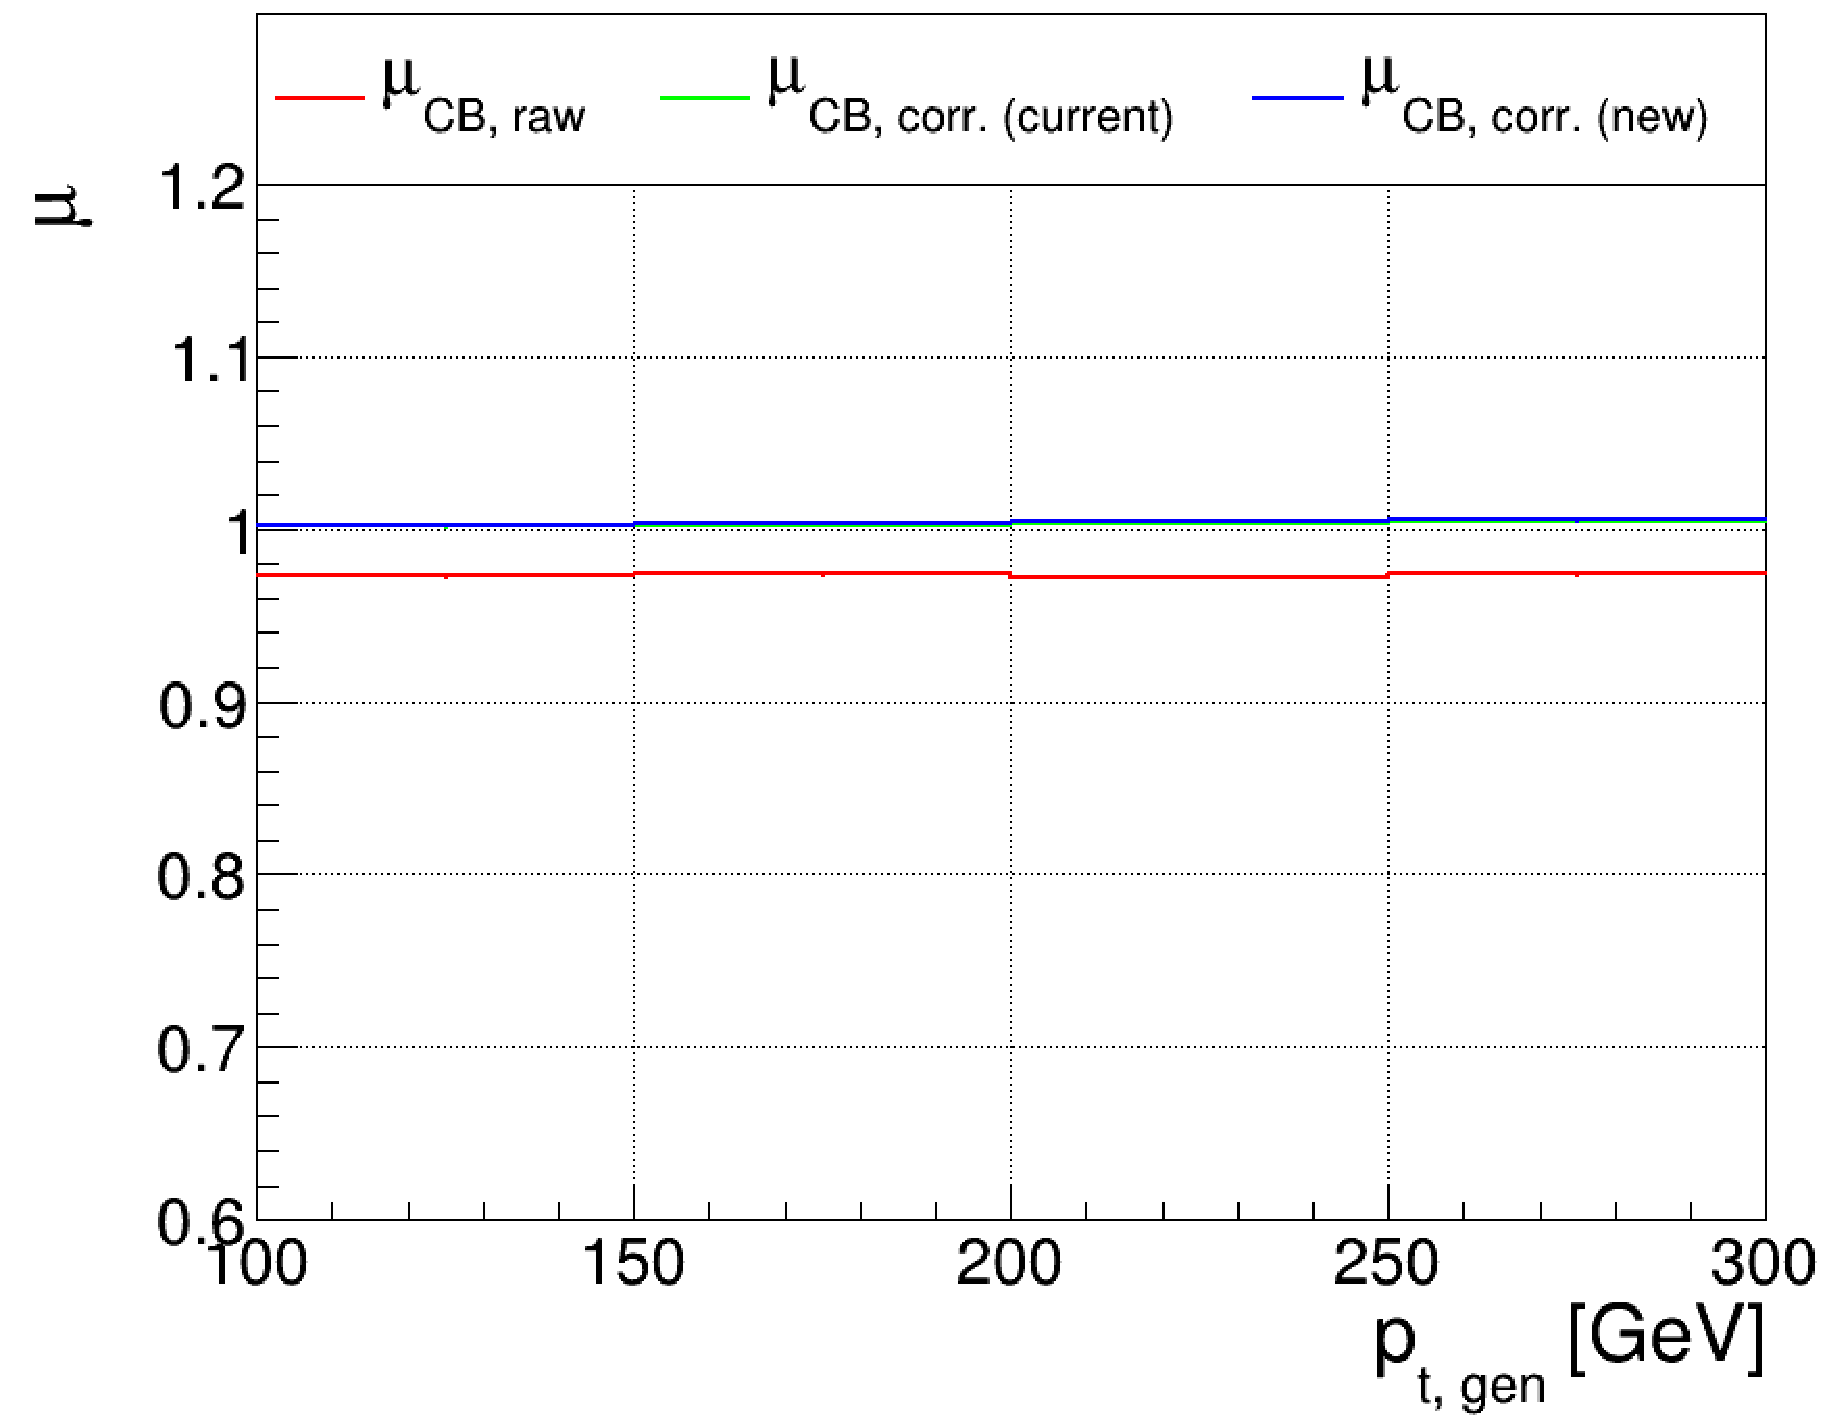
\includegraphics[width=0.495\textwidth]{./ECAL_plots/plotsNoPU/EE/pdf/FULL/GENPT/EEFULL_GENPT_0100_0300_MuOverBins.pdf}
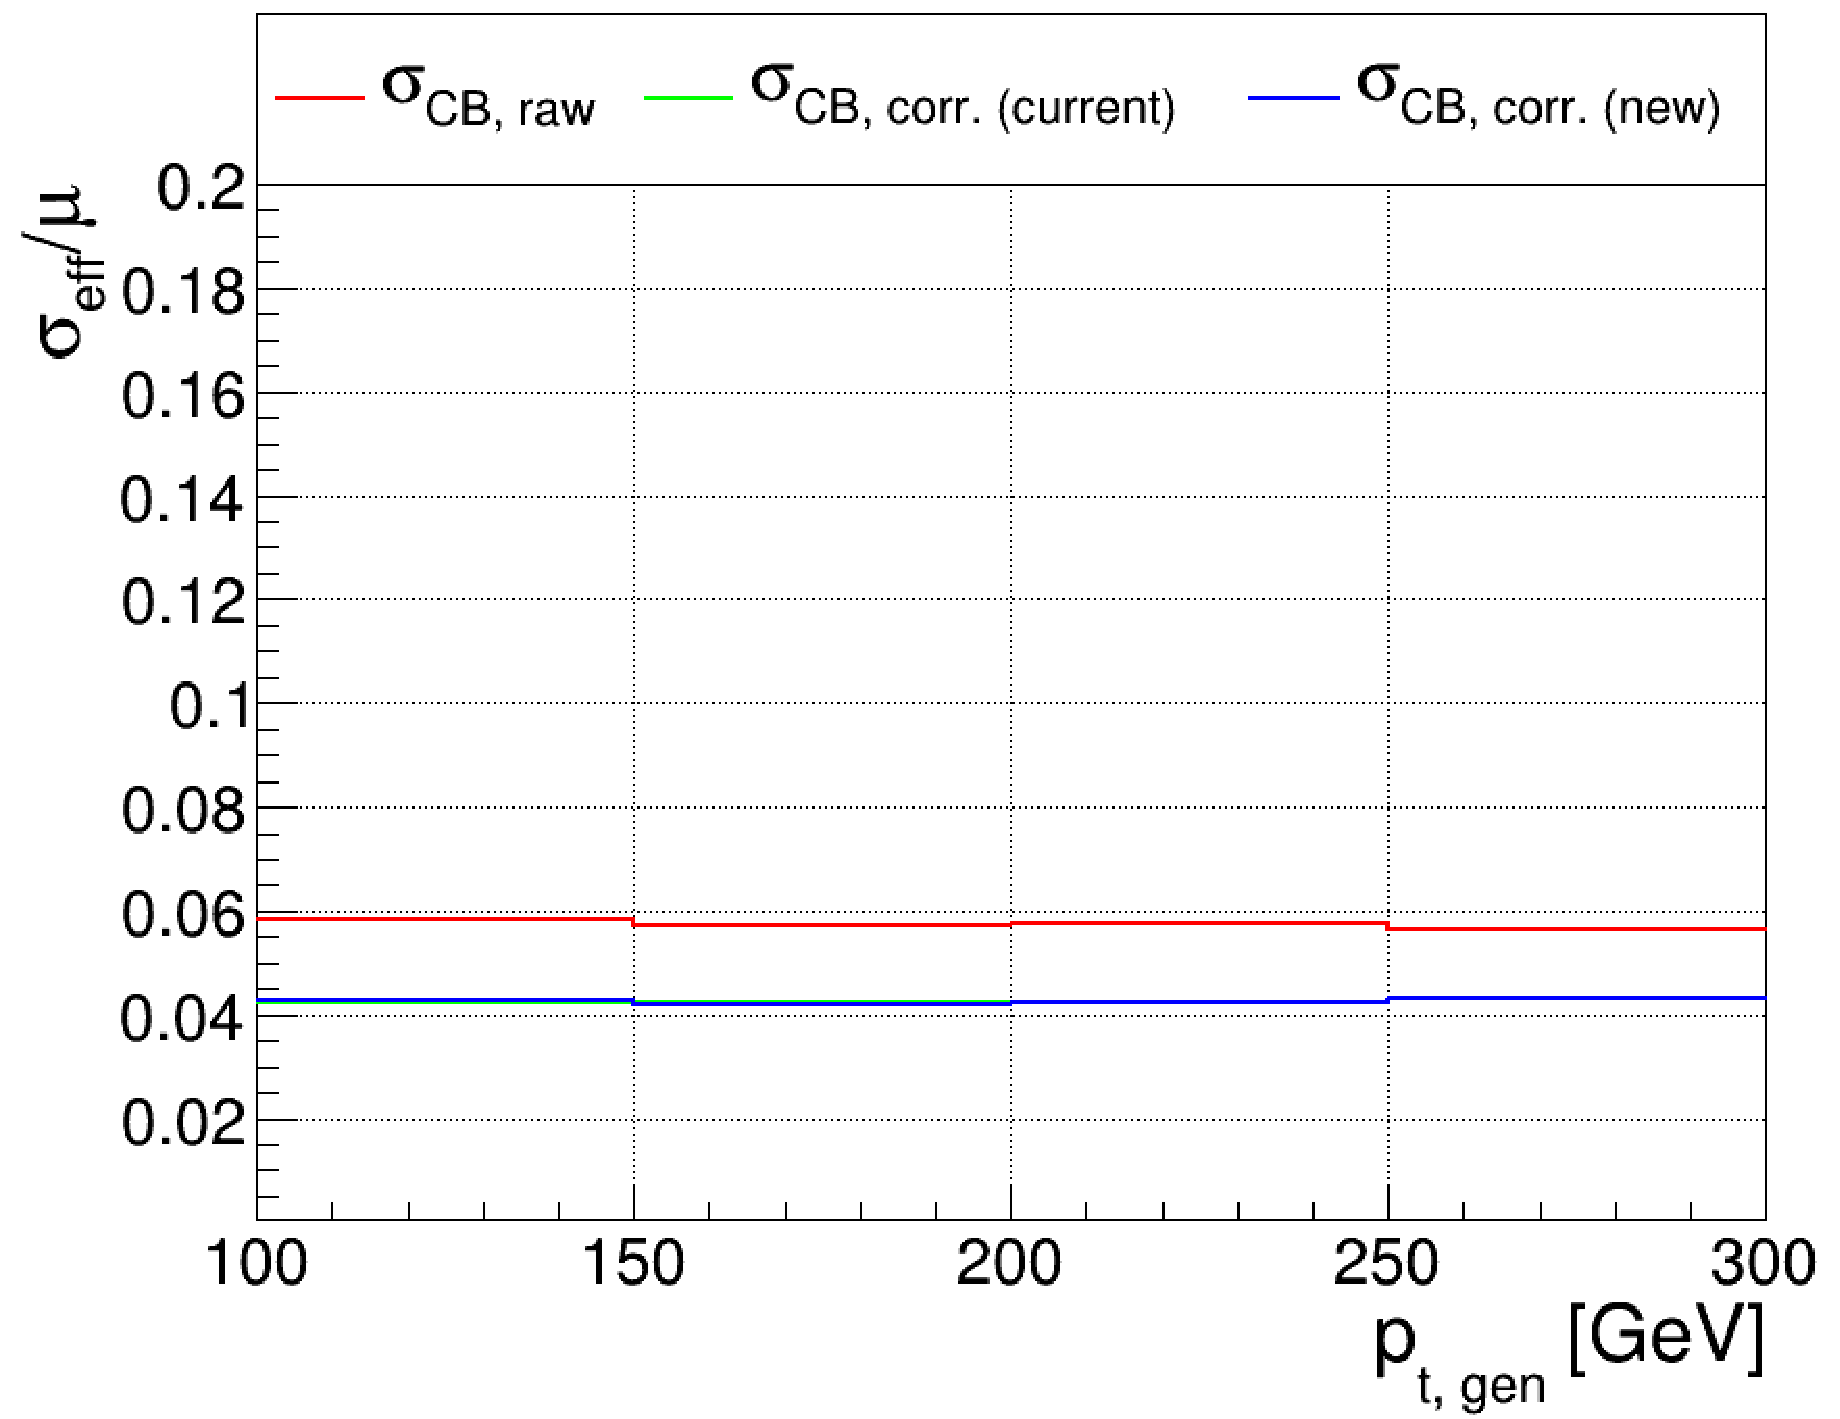
\includegraphics[width=0.495\textwidth]{./ECAL_plots/plotsNoPU/EE/pdf/FULL/GENPT/EEFULL_GENPT_0100_0300_EffSigmaOverBins.pdf}
%\caption{EE - Full Readout pt 100-300}
%\end{figure}
%\begin{figure}
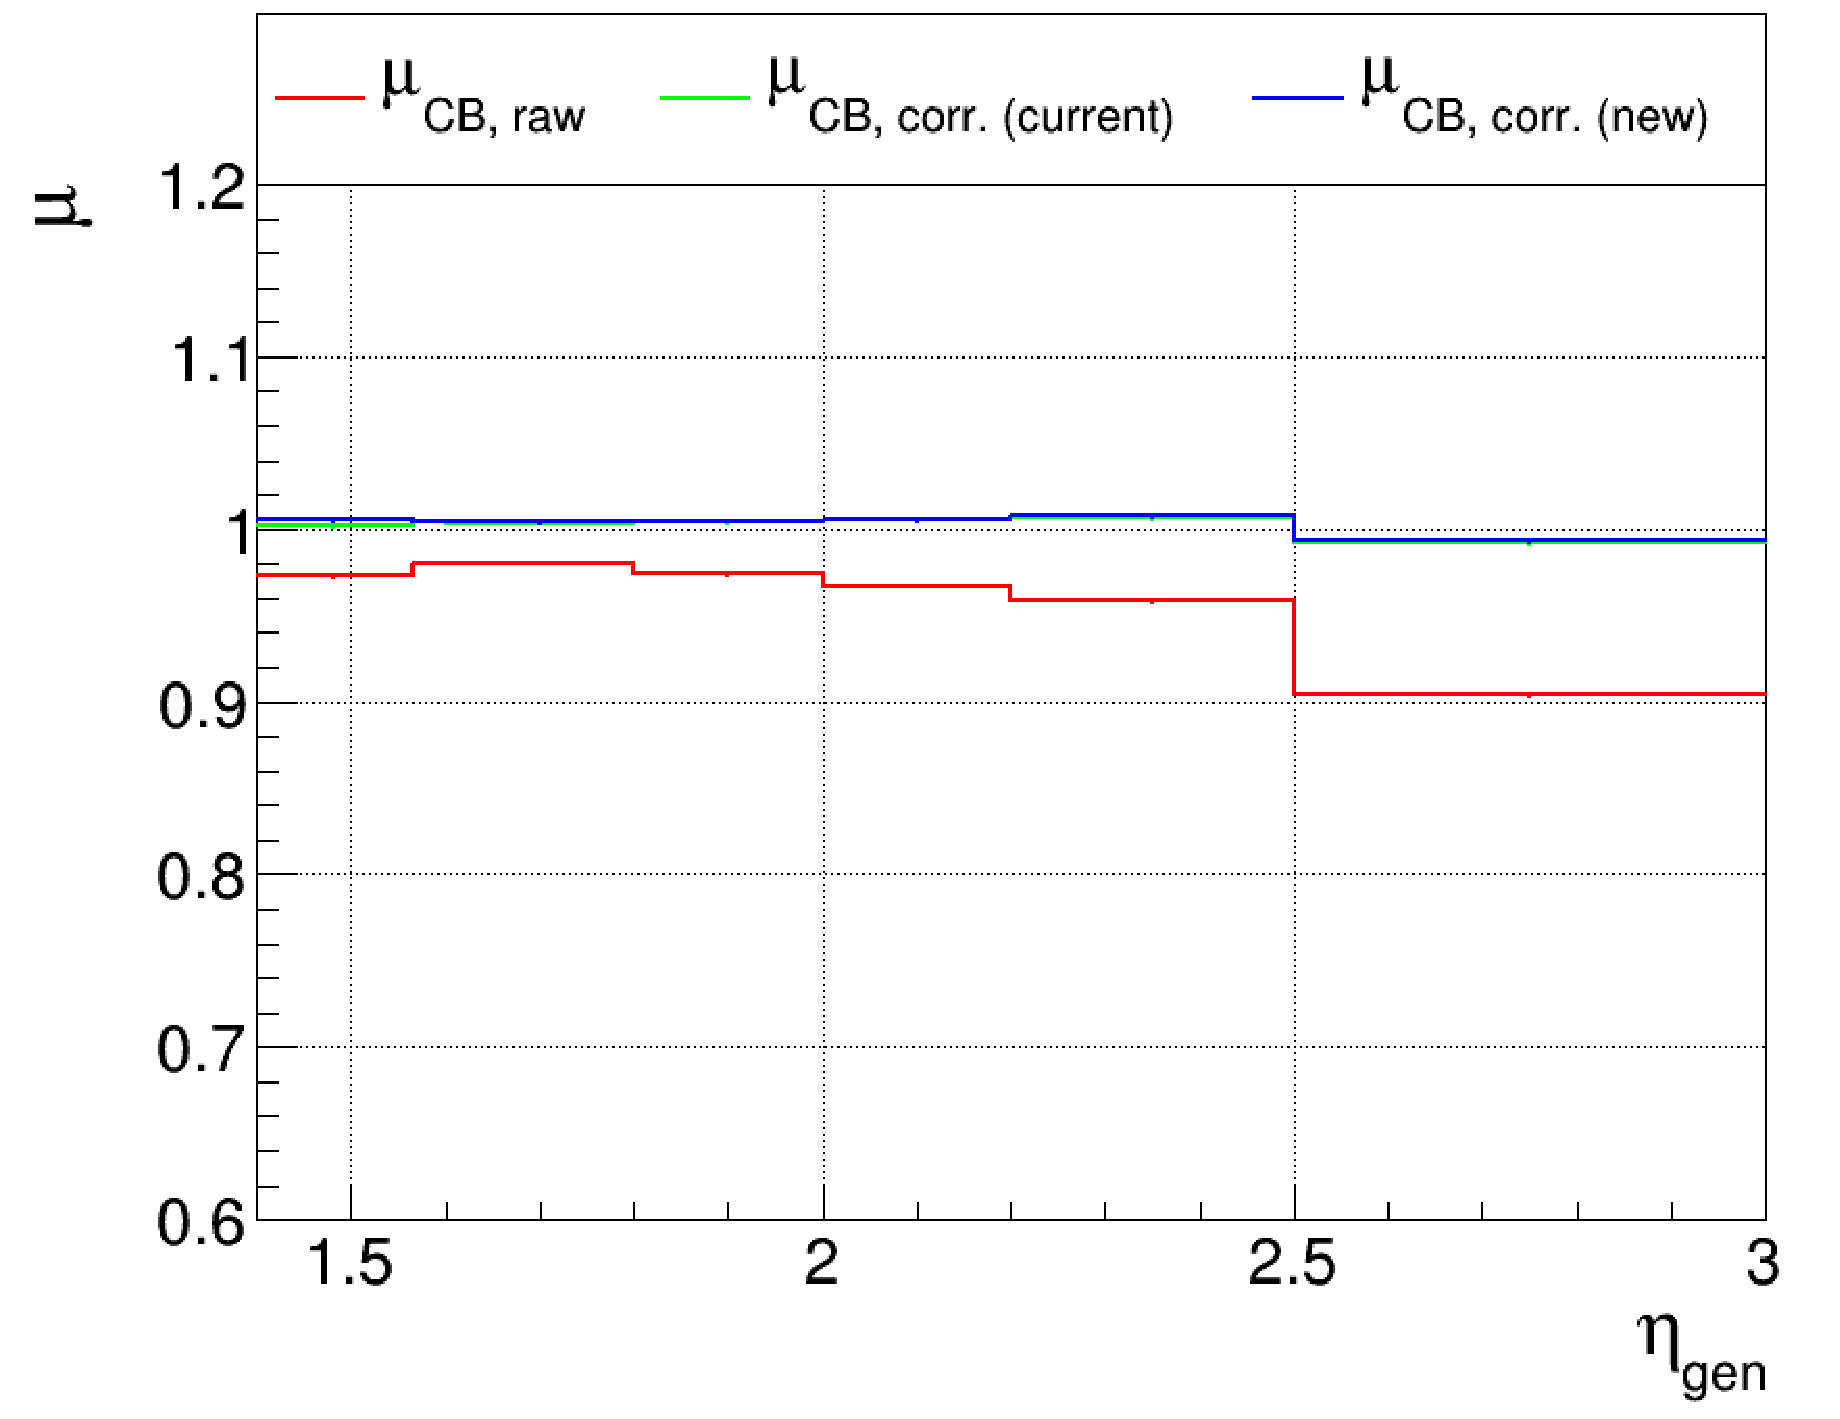
\includegraphics[width=0.495\textwidth]{./ECAL_plots/plotsNoPU/EE/pdf/FULL/GENETA/EEFULL_GENETA_0100_0300_MuOverBins.pdf}
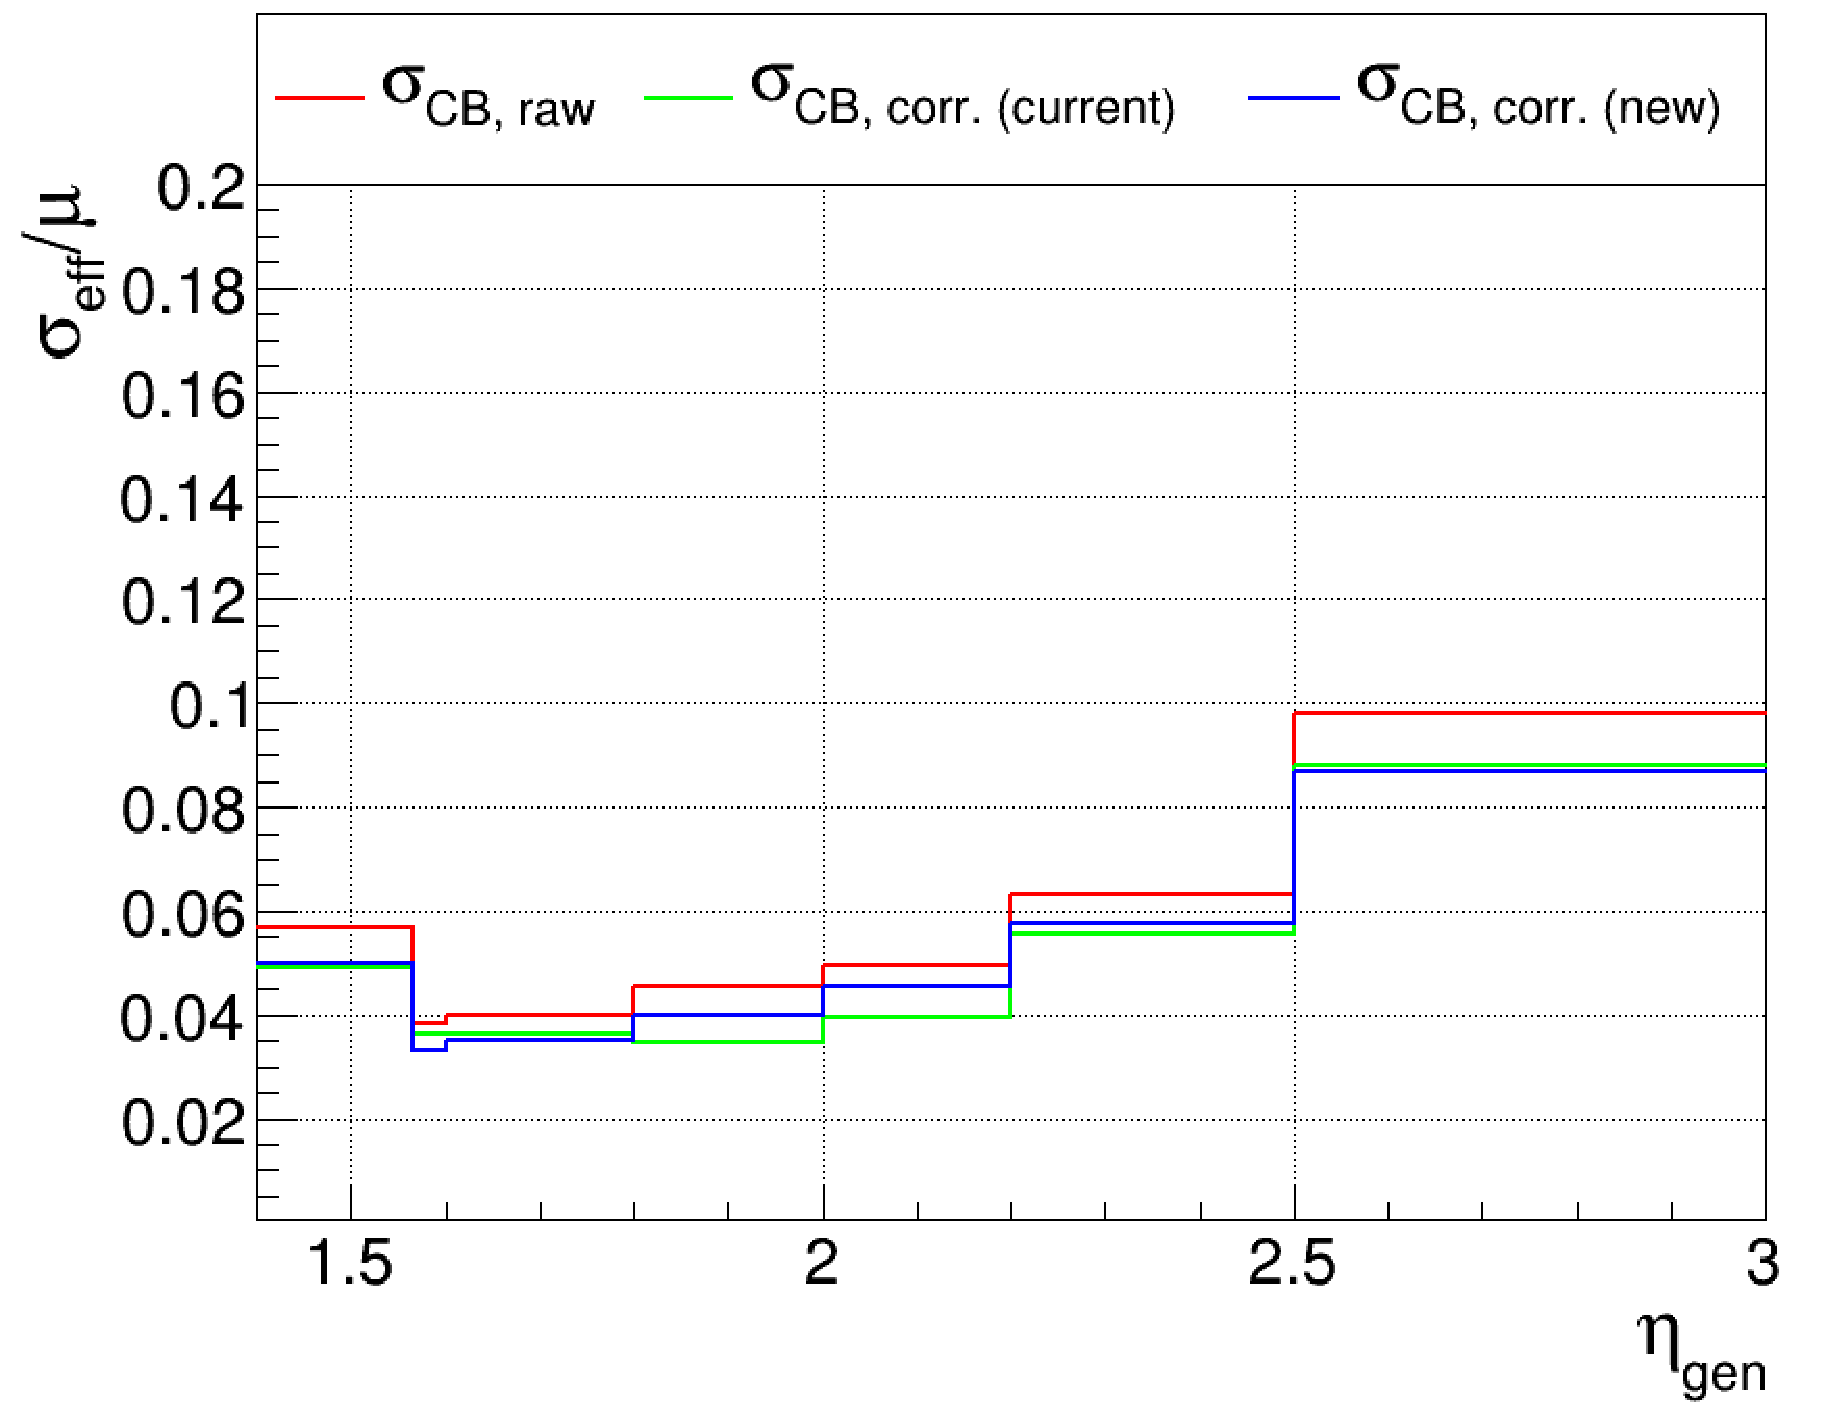
\includegraphics[width=0.495\textwidth]{./ECAL_plots/plotsNoPU/EE/pdf/FULL/GENETA/EEFULL_GENETA_0005_0020_EffSigmaOverBins.pdf}
\caption{EE - Full Readout pt 100-300}
\end{figure}





\begin{figure}
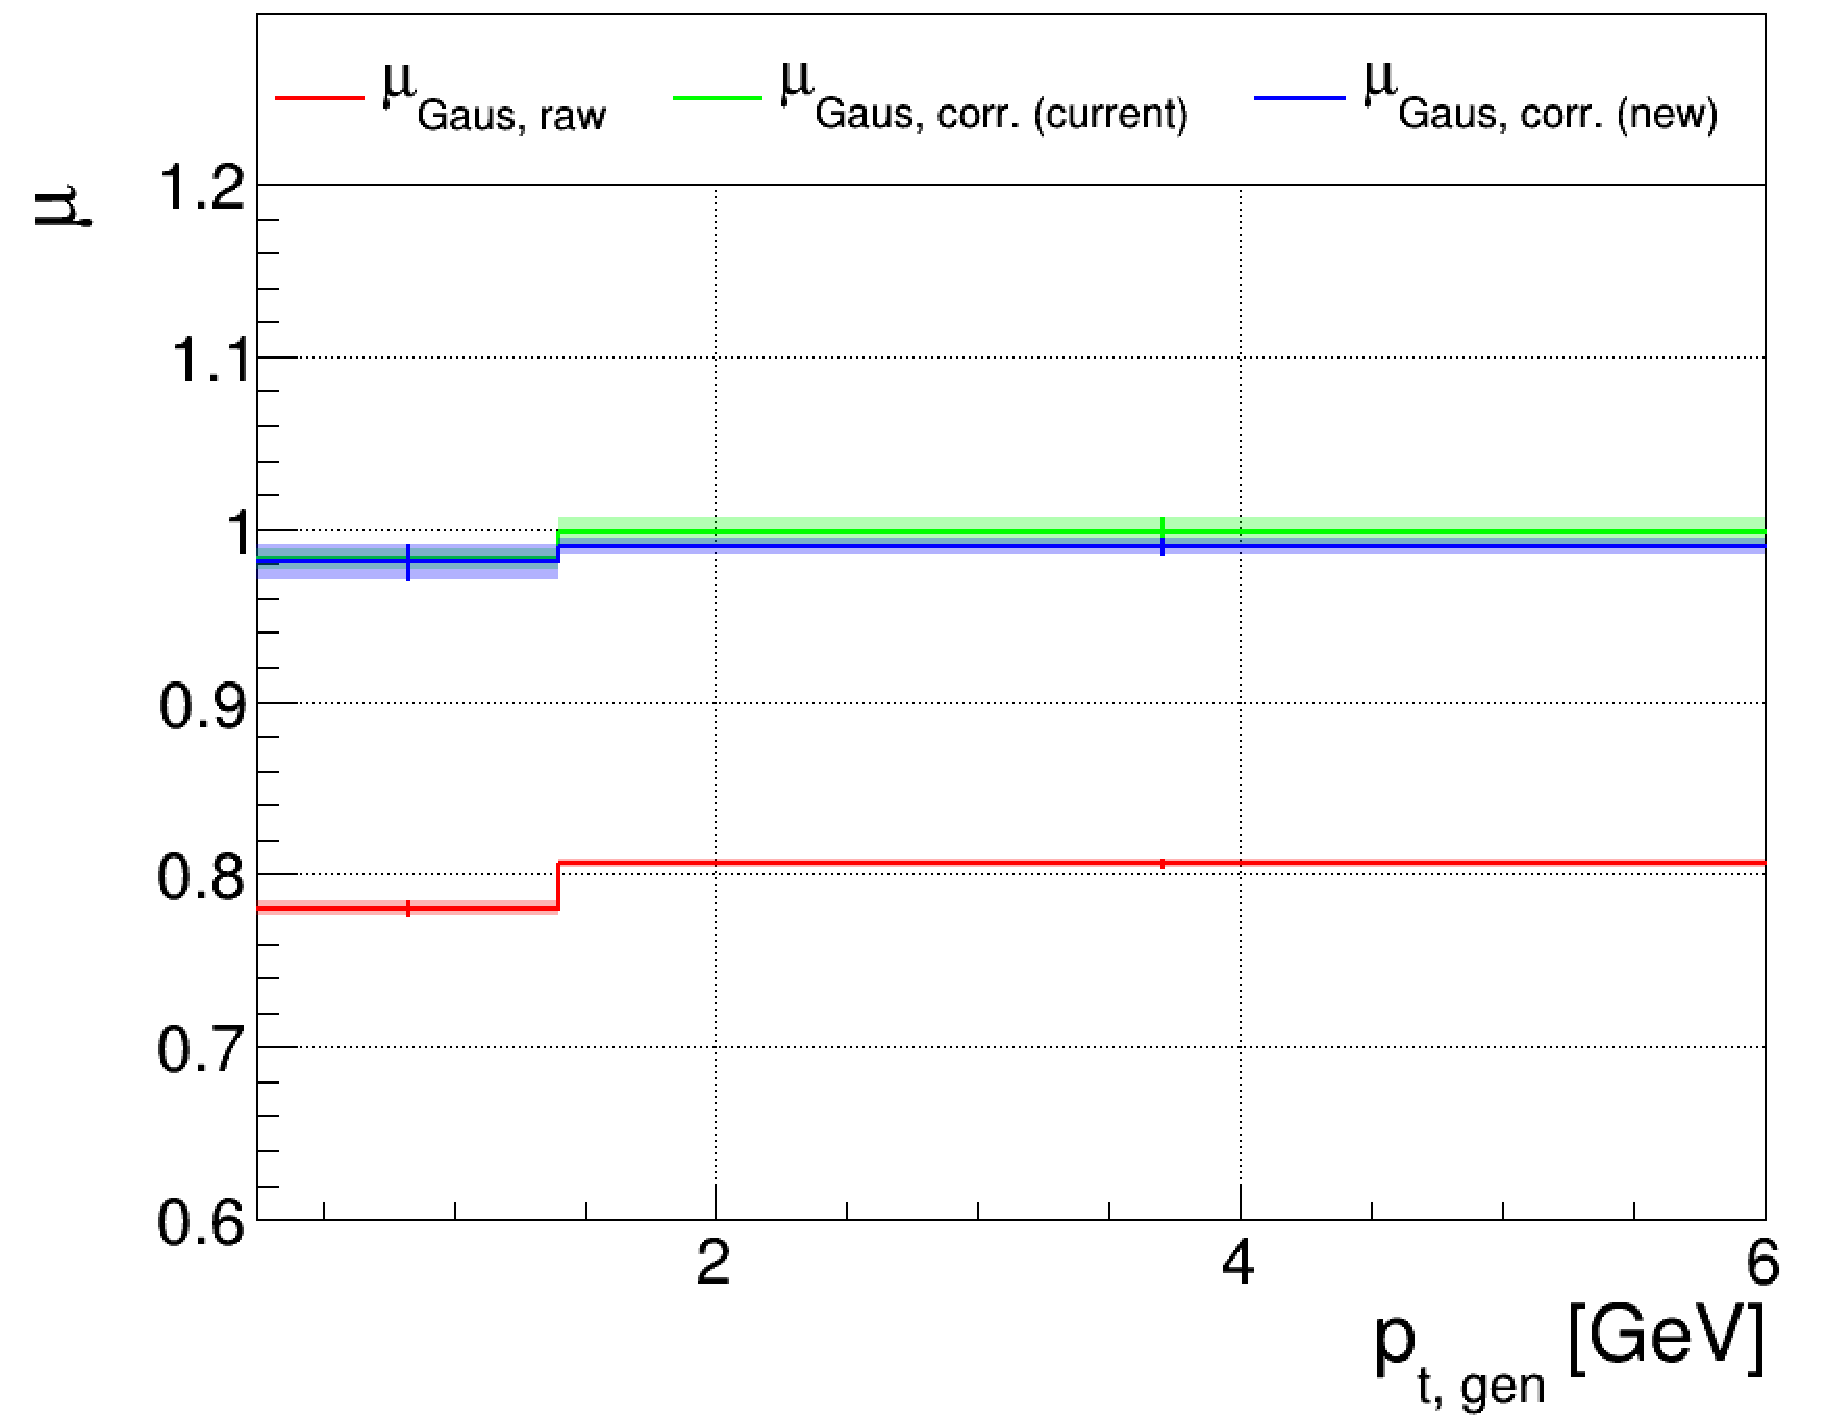
\includegraphics[width=0.495\textwidth]{./plots_pdf/ECAL_plots/plotsNoPU/EE/pdf/ZS/GENPT/EEZS_GENPT_0000_0006_MuOverBins.pdf}
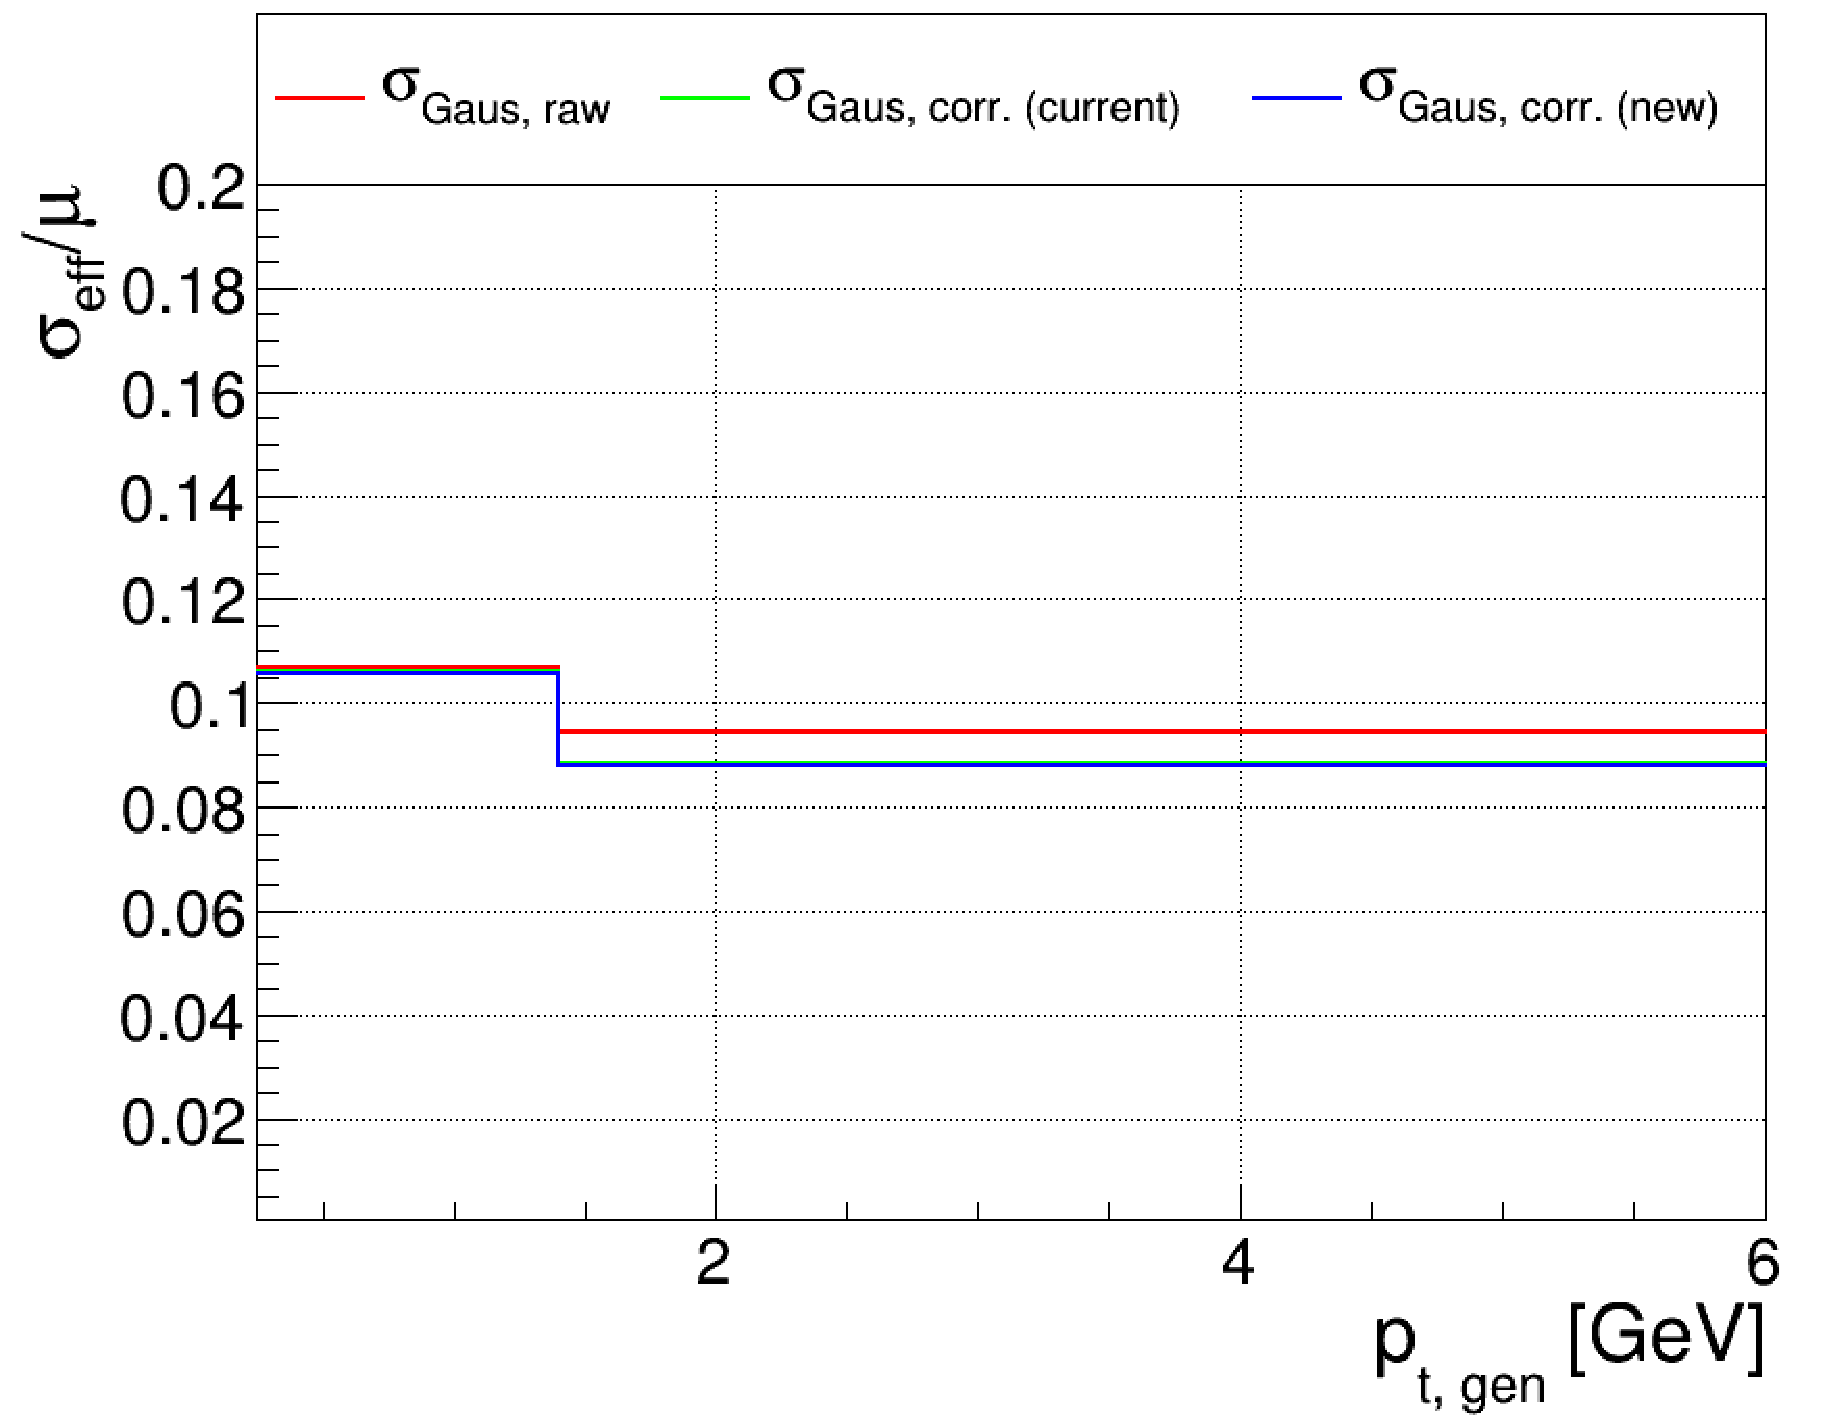
\includegraphics[width=0.495\textwidth]{./plots_pdf/ECAL_plots/plotsNoPU/EE/pdf/ZS/GENPT/EEZS_GENPT_0000_0006_EffSigmaOverBins.pdf}

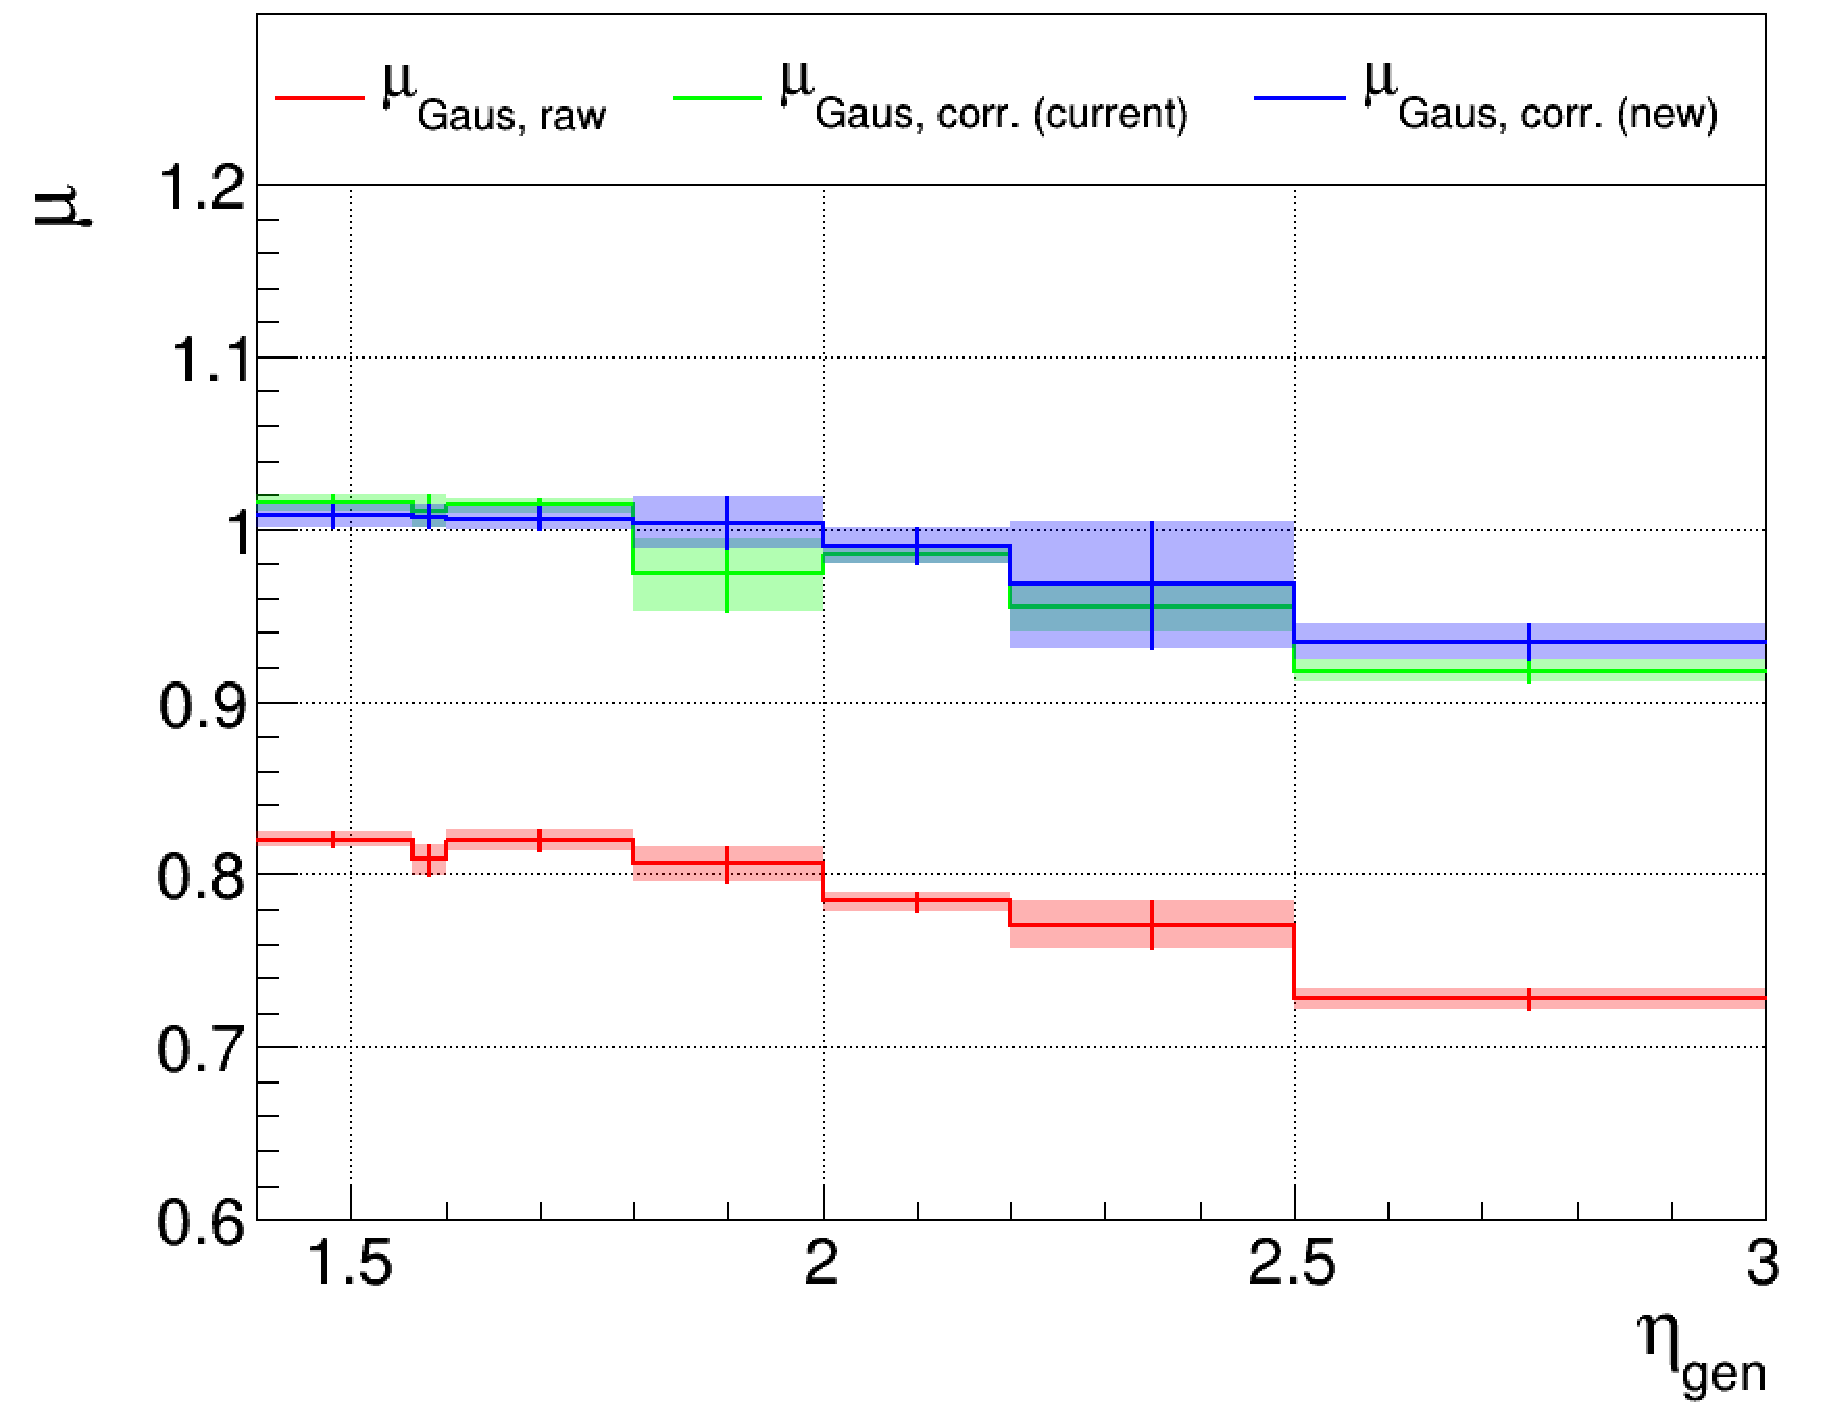
\includegraphics[width=0.495\textwidth]{./plots_pdf/ECAL_plots/plotsNoPU/EE/pdf/ZS/GENETA/EEZS_GENETA_0000_0006_MuOverBins.pdf}
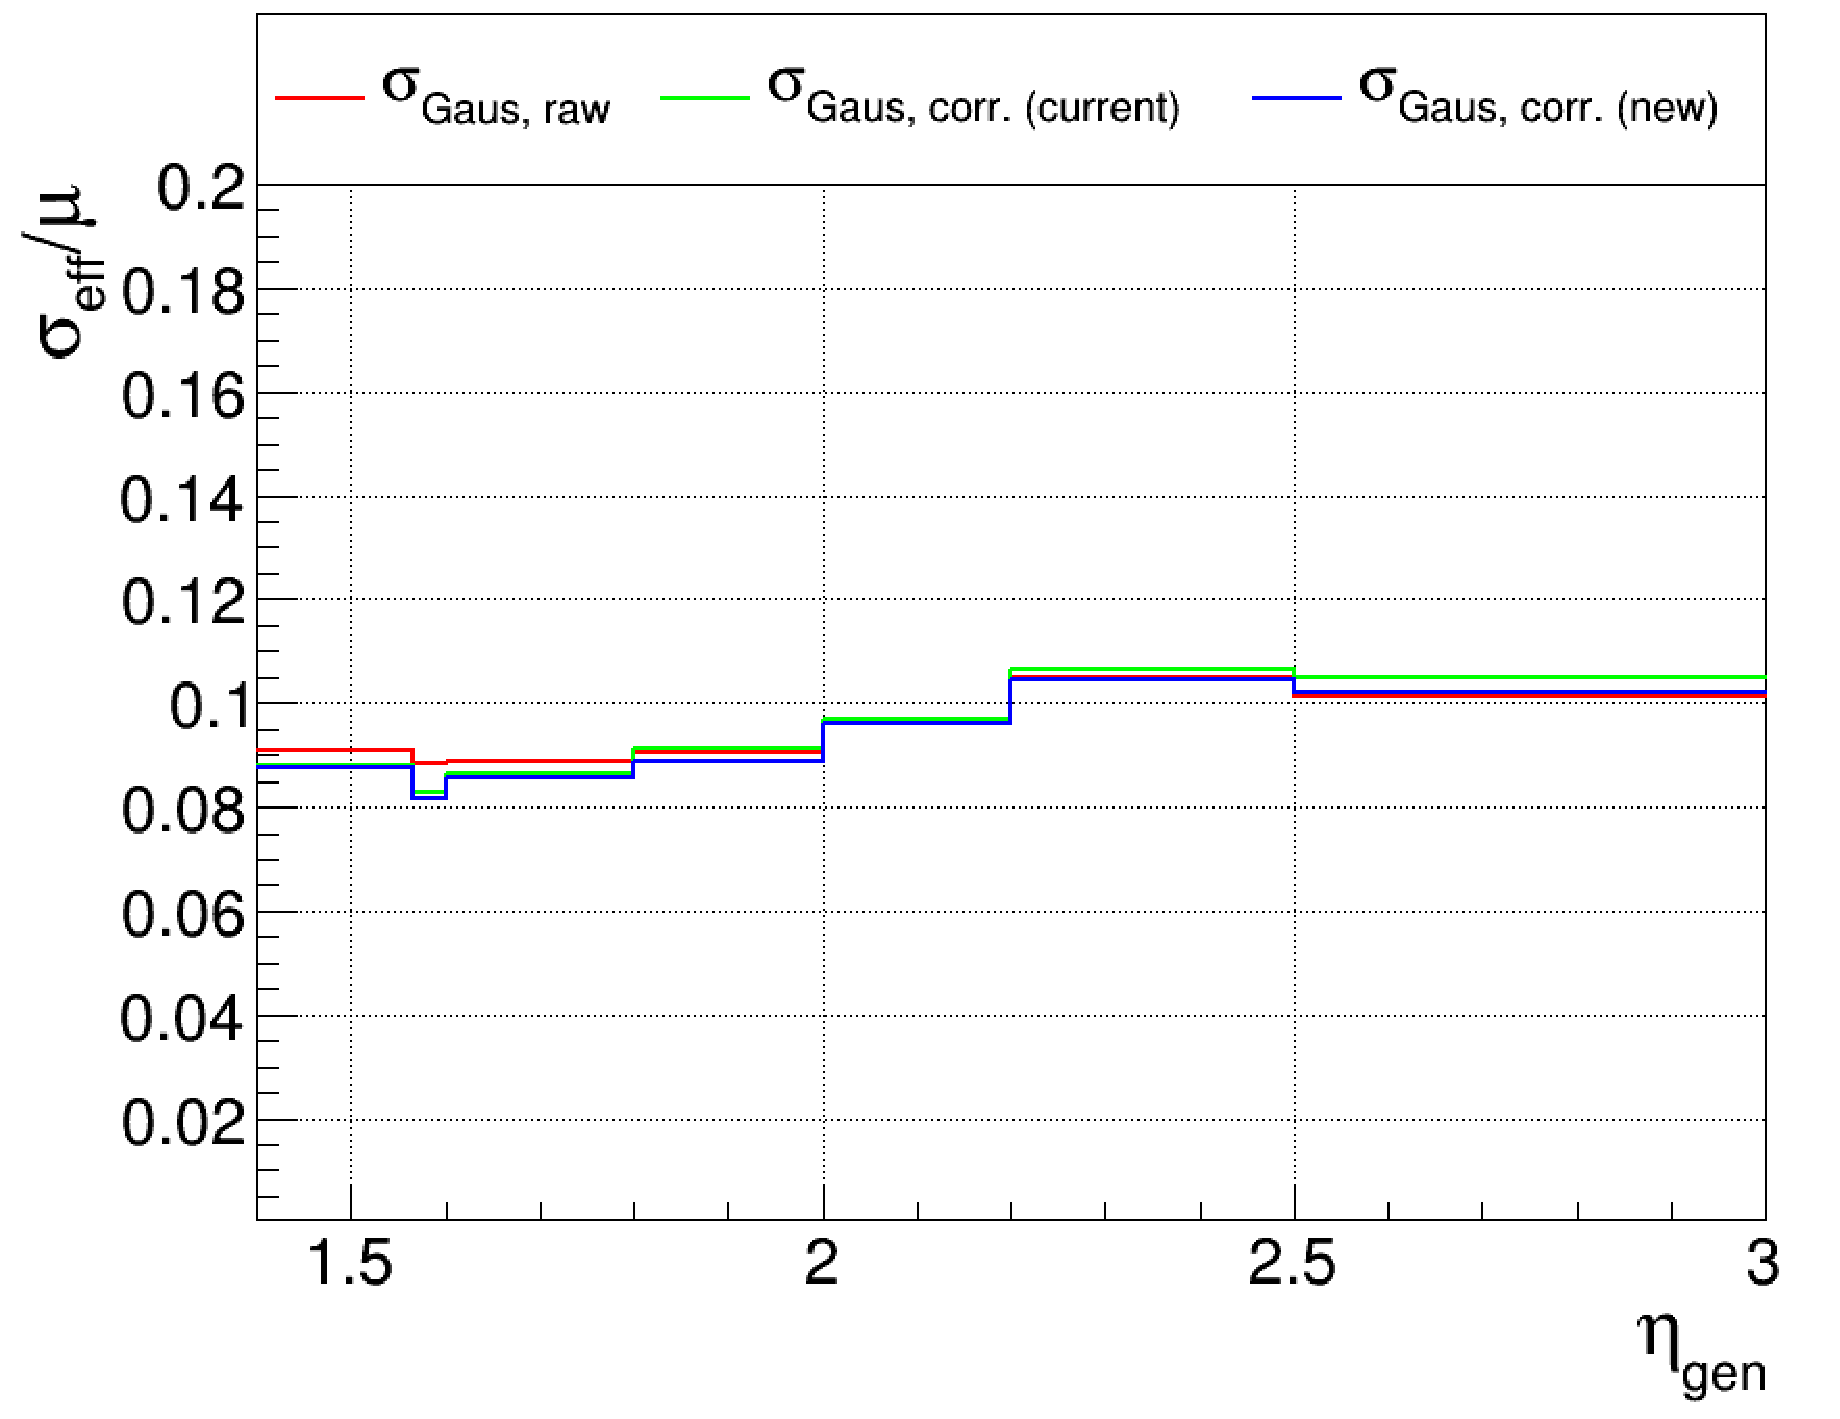
\includegraphics[width=0.495\textwidth]{./plots_pdf/ECAL_plots/plotsNoPU/EE/pdf/ZS/GENETA/EEZS_GENETA_0000_0006_EffSigmaOverBins.pdf}
\caption[$\mu$ ($\sigma_\mathrm{eff}$) vs \pt of PF ECAL cluster - EE ZS readout NoPU scenario]{Mean response (resolution) defined by Raw PF ECAL clusters (red), the calibration derived earlier in Ru\
n3 based on 126X (green), and the new correction from 2024 simulation sample based on 133X (blue).\pt 0--6\GeV in EE region ZS Readout NOPU scenario.}
\end{figure}

%% %\begin{figure}
%% 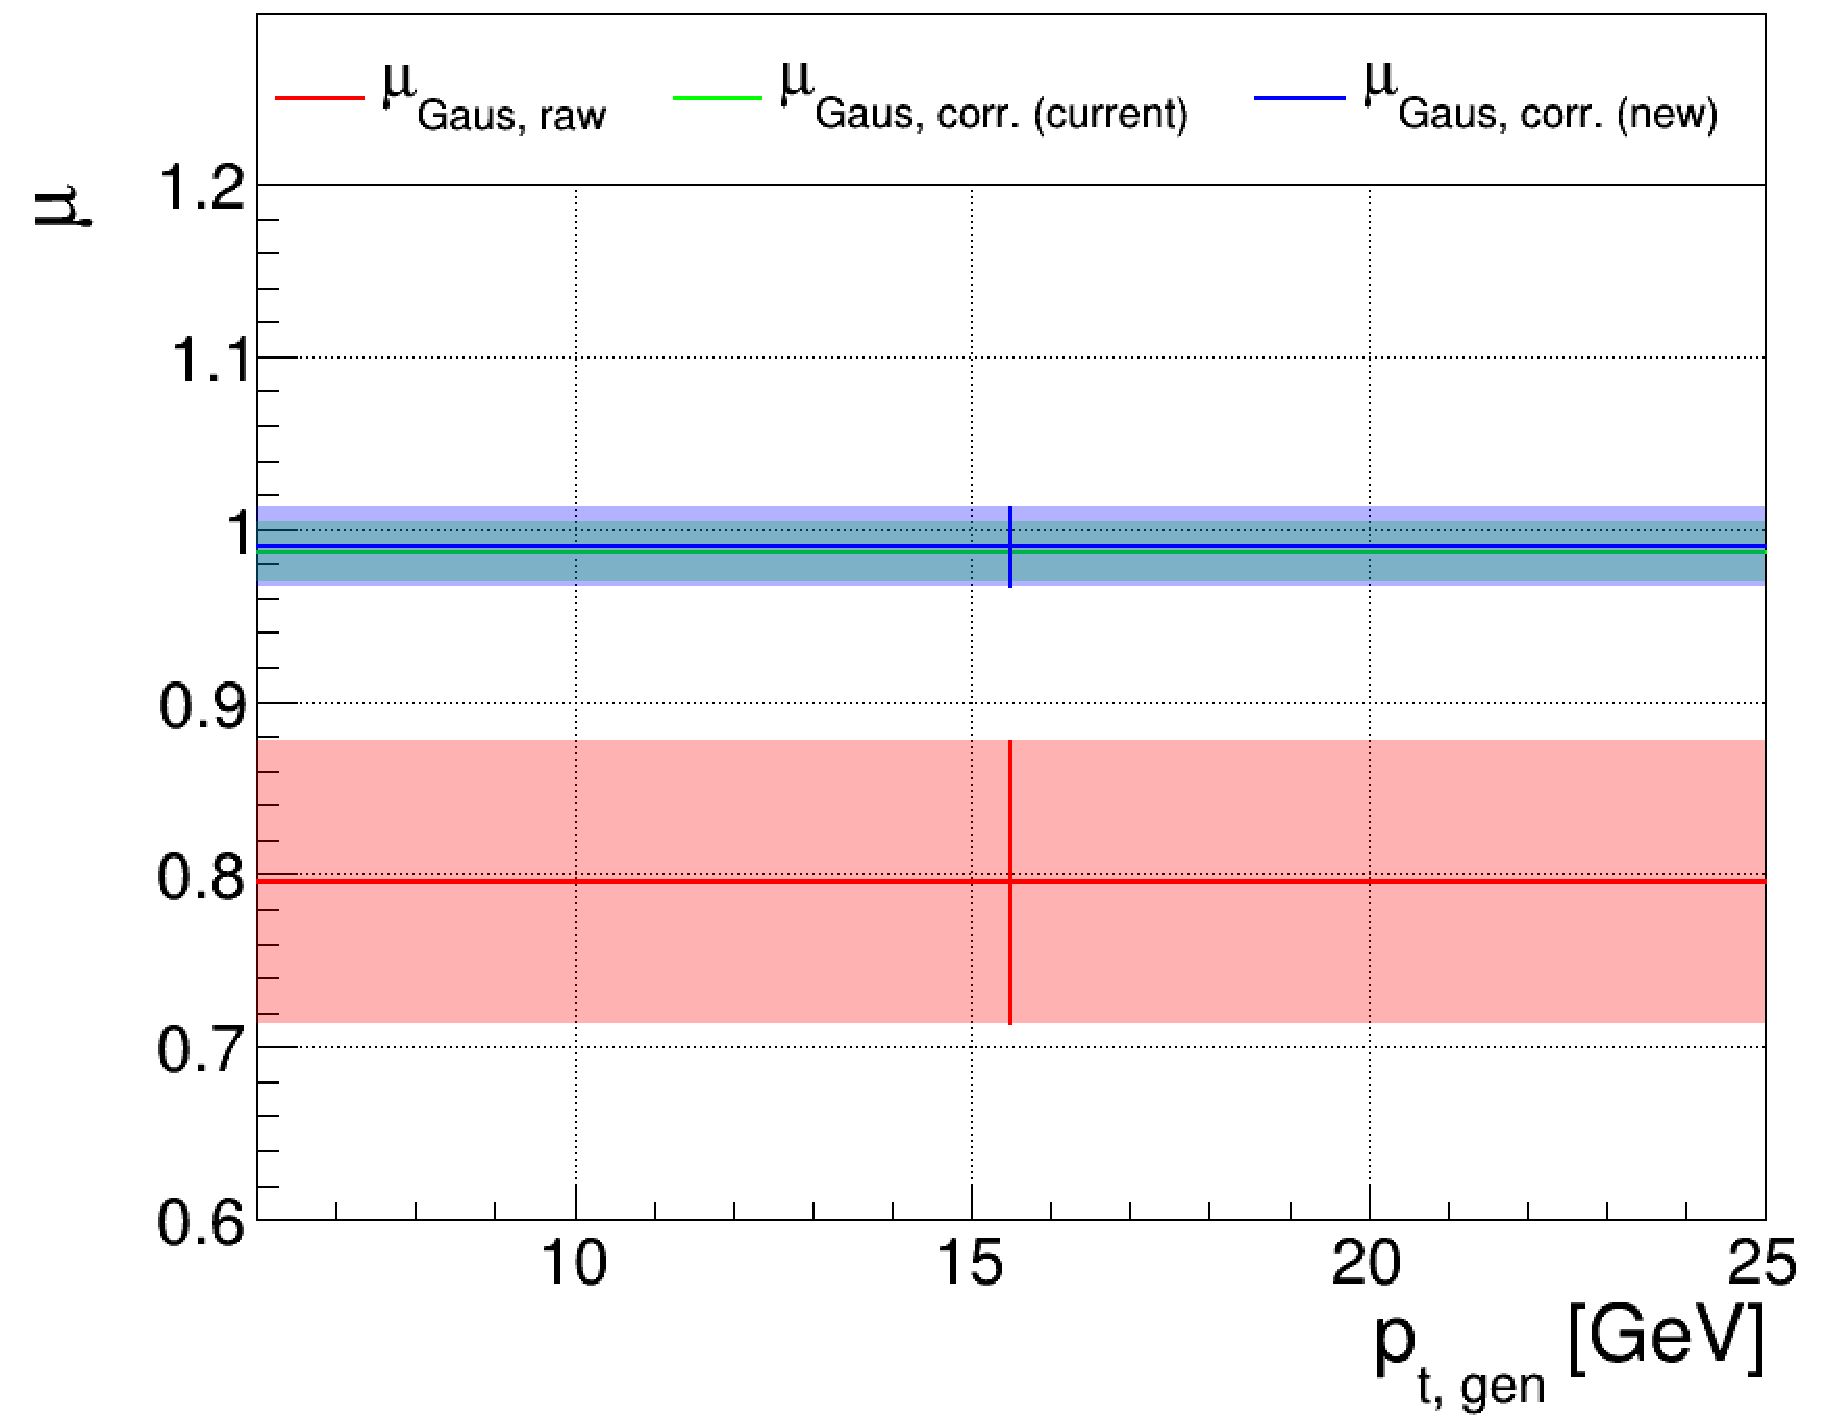
\includegraphics[width=0.495\textwidth]{./plots_pdf/ECAL_plots/plotsNoPU/EE/pdf/ZS/GENPT/EEZS_GENPT_0006_0025_MuOverBins.pdf}
%% 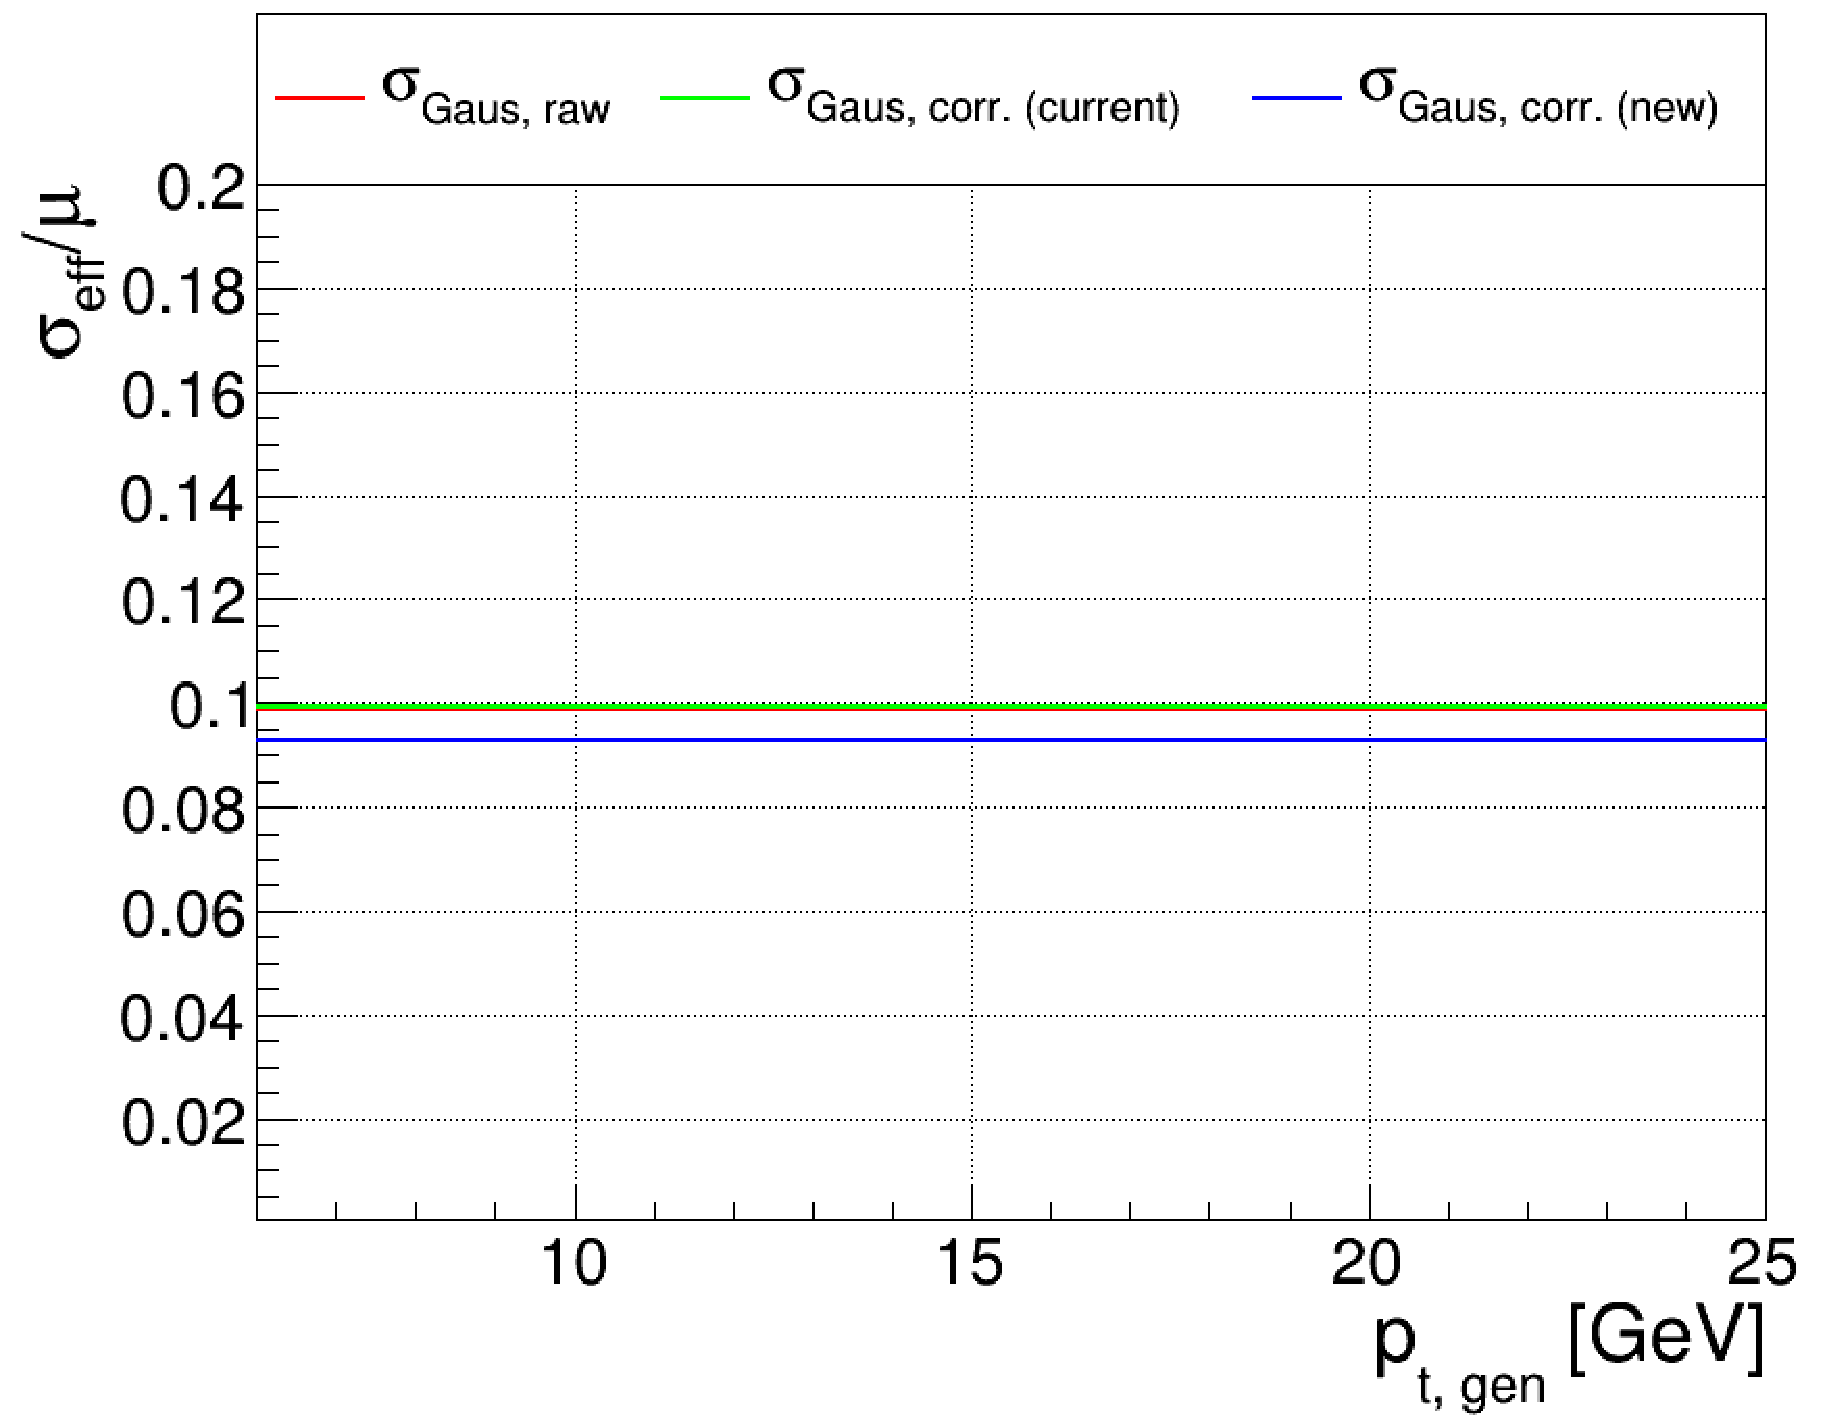
\includegraphics[width=0.495\textwidth]{./plots_pdf/ECAL_plots/plotsNoPU/EE/pdf/ZS/GENPT/EEZS_GENPT_0006_0025_EffSigmaOverBins.pdf}
%% %\caption{EE - ZS Readout pt 6-25}
%% %\end{figure}
%% %\begin{figure}
%% 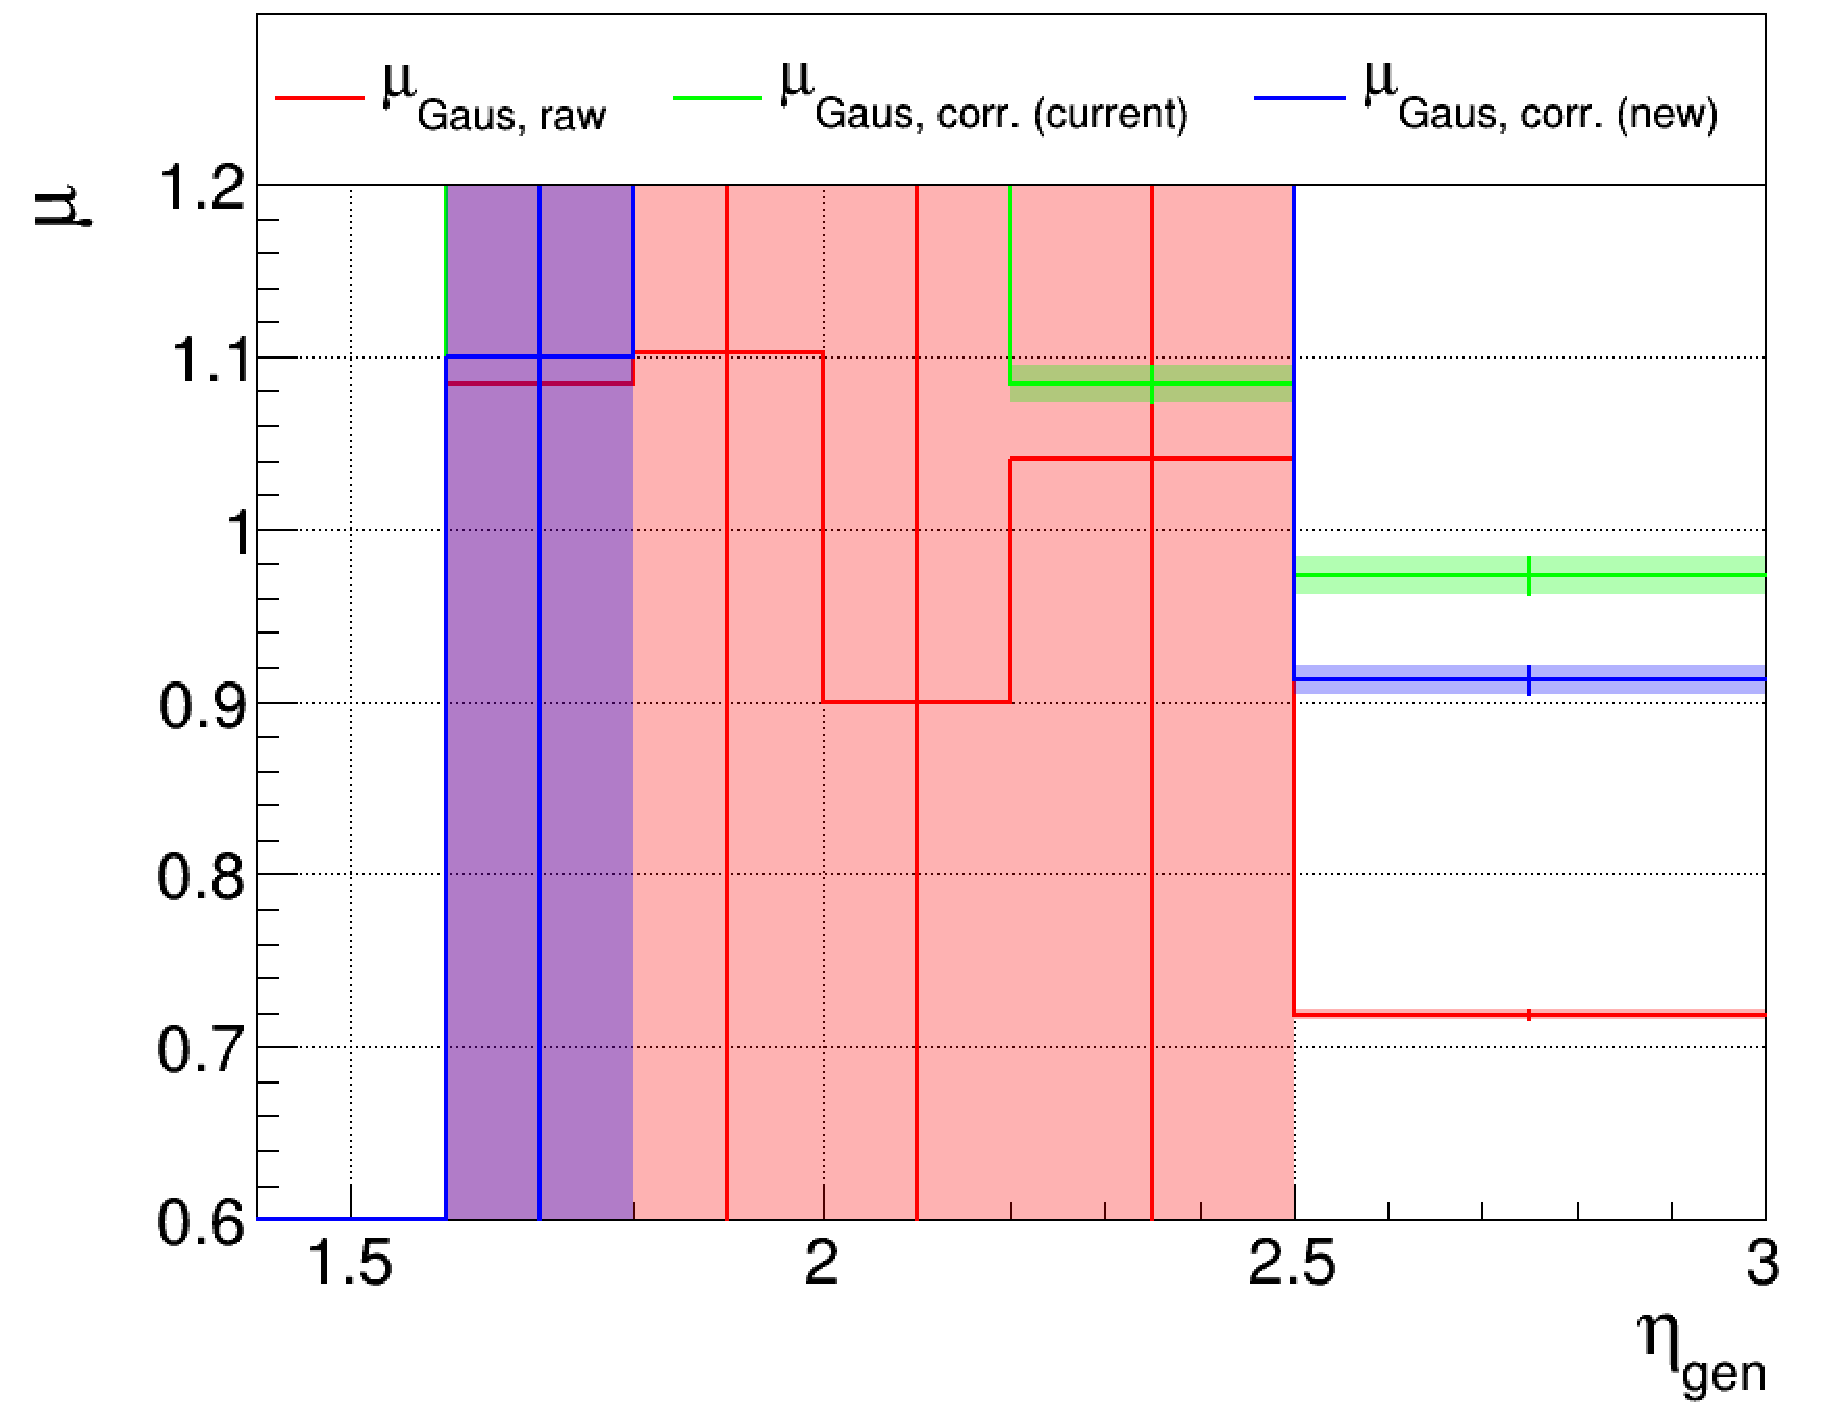
\includegraphics[width=0.495\textwidth]{./plots_pdf/ECAL_plots/plotsNoPU/EE/pdf/ZS/GENETA/EEZS_GENETA_0006_0025_MuOverBins.pdf}
%% %\includegraphics[width=0.495\textwidth]{./ECAL_plots/plotsNoPU/EE/pdf/ZS/GENETA/EEZS_GENETA_0006_0025_EffSigmaOverBins.pdf}
%% \caption{EE - ZS Readout \pt 6-25}
%% \end{figure}





Second for PU samples plots in EB region:
\begin{figure}
\includegraphics[width=0.495\textwidth]{./plots_pdf/ECAL_plots/plotsPU/EB/FULL/pdf/GENPT/EBFULL_GENPT_0005_0020_MuOverBins.pdf}
\includegraphics[width=0.495\textwidth]{./plots_pdf/ECAL_plots/plotsPU/EB/FULL/pdf/GENPT/EBFULL_GENPT_0005_0020_EffSigmaOverBins.pdf}
%\caption{EB - Full Readout pt 5-20}
%\end{figure}
%\begin{figure}
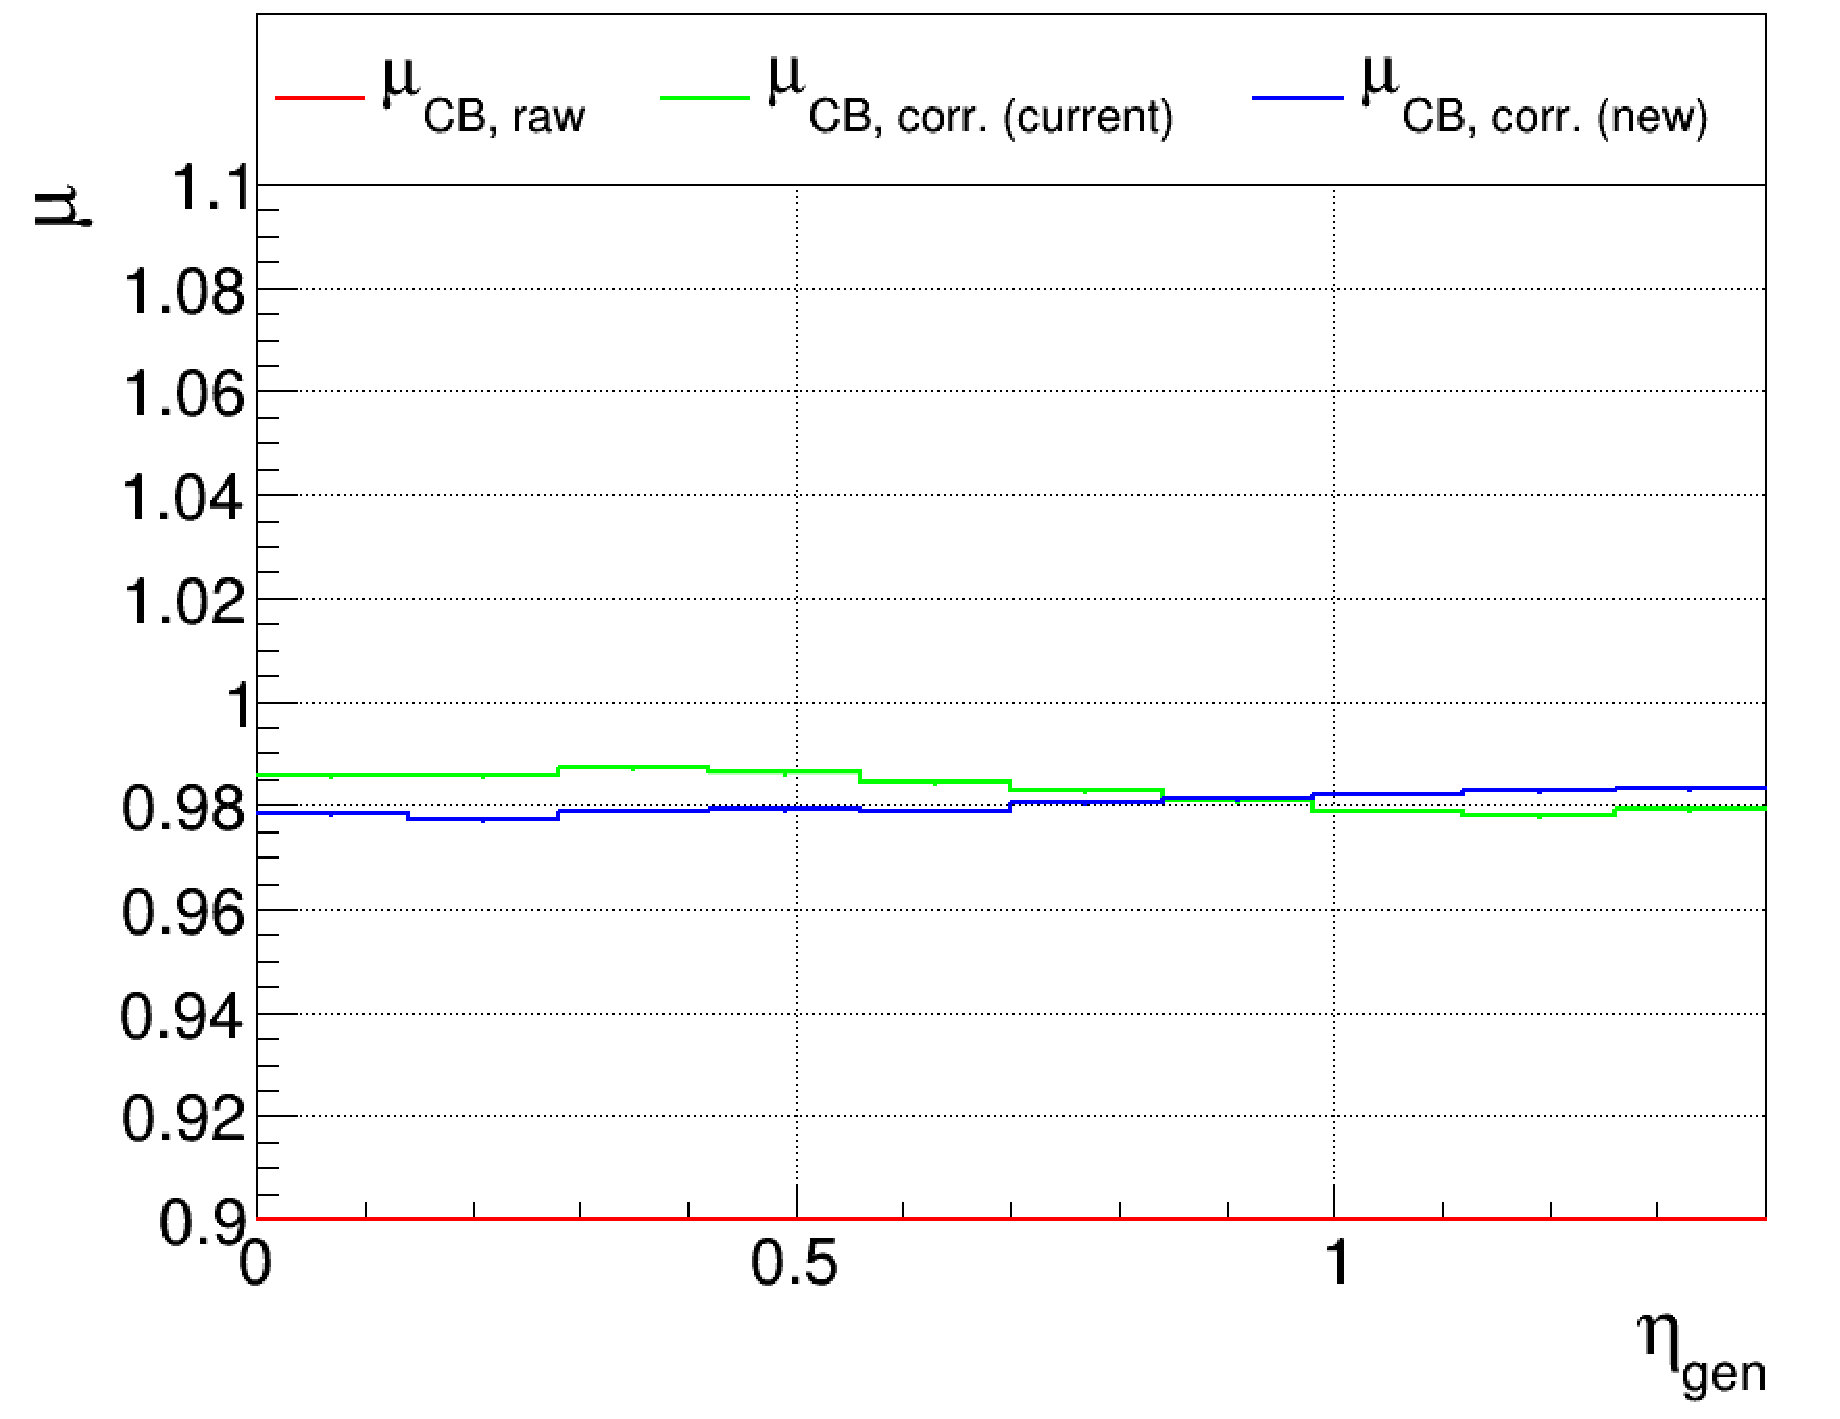
\includegraphics[width=0.495\textwidth]{./plots_pdf/ECAL_plots/plotsPU/EB/FULL/pdf/GENETA/EBFULL_GENETA_0005_0020_MuOverBins.pdf}
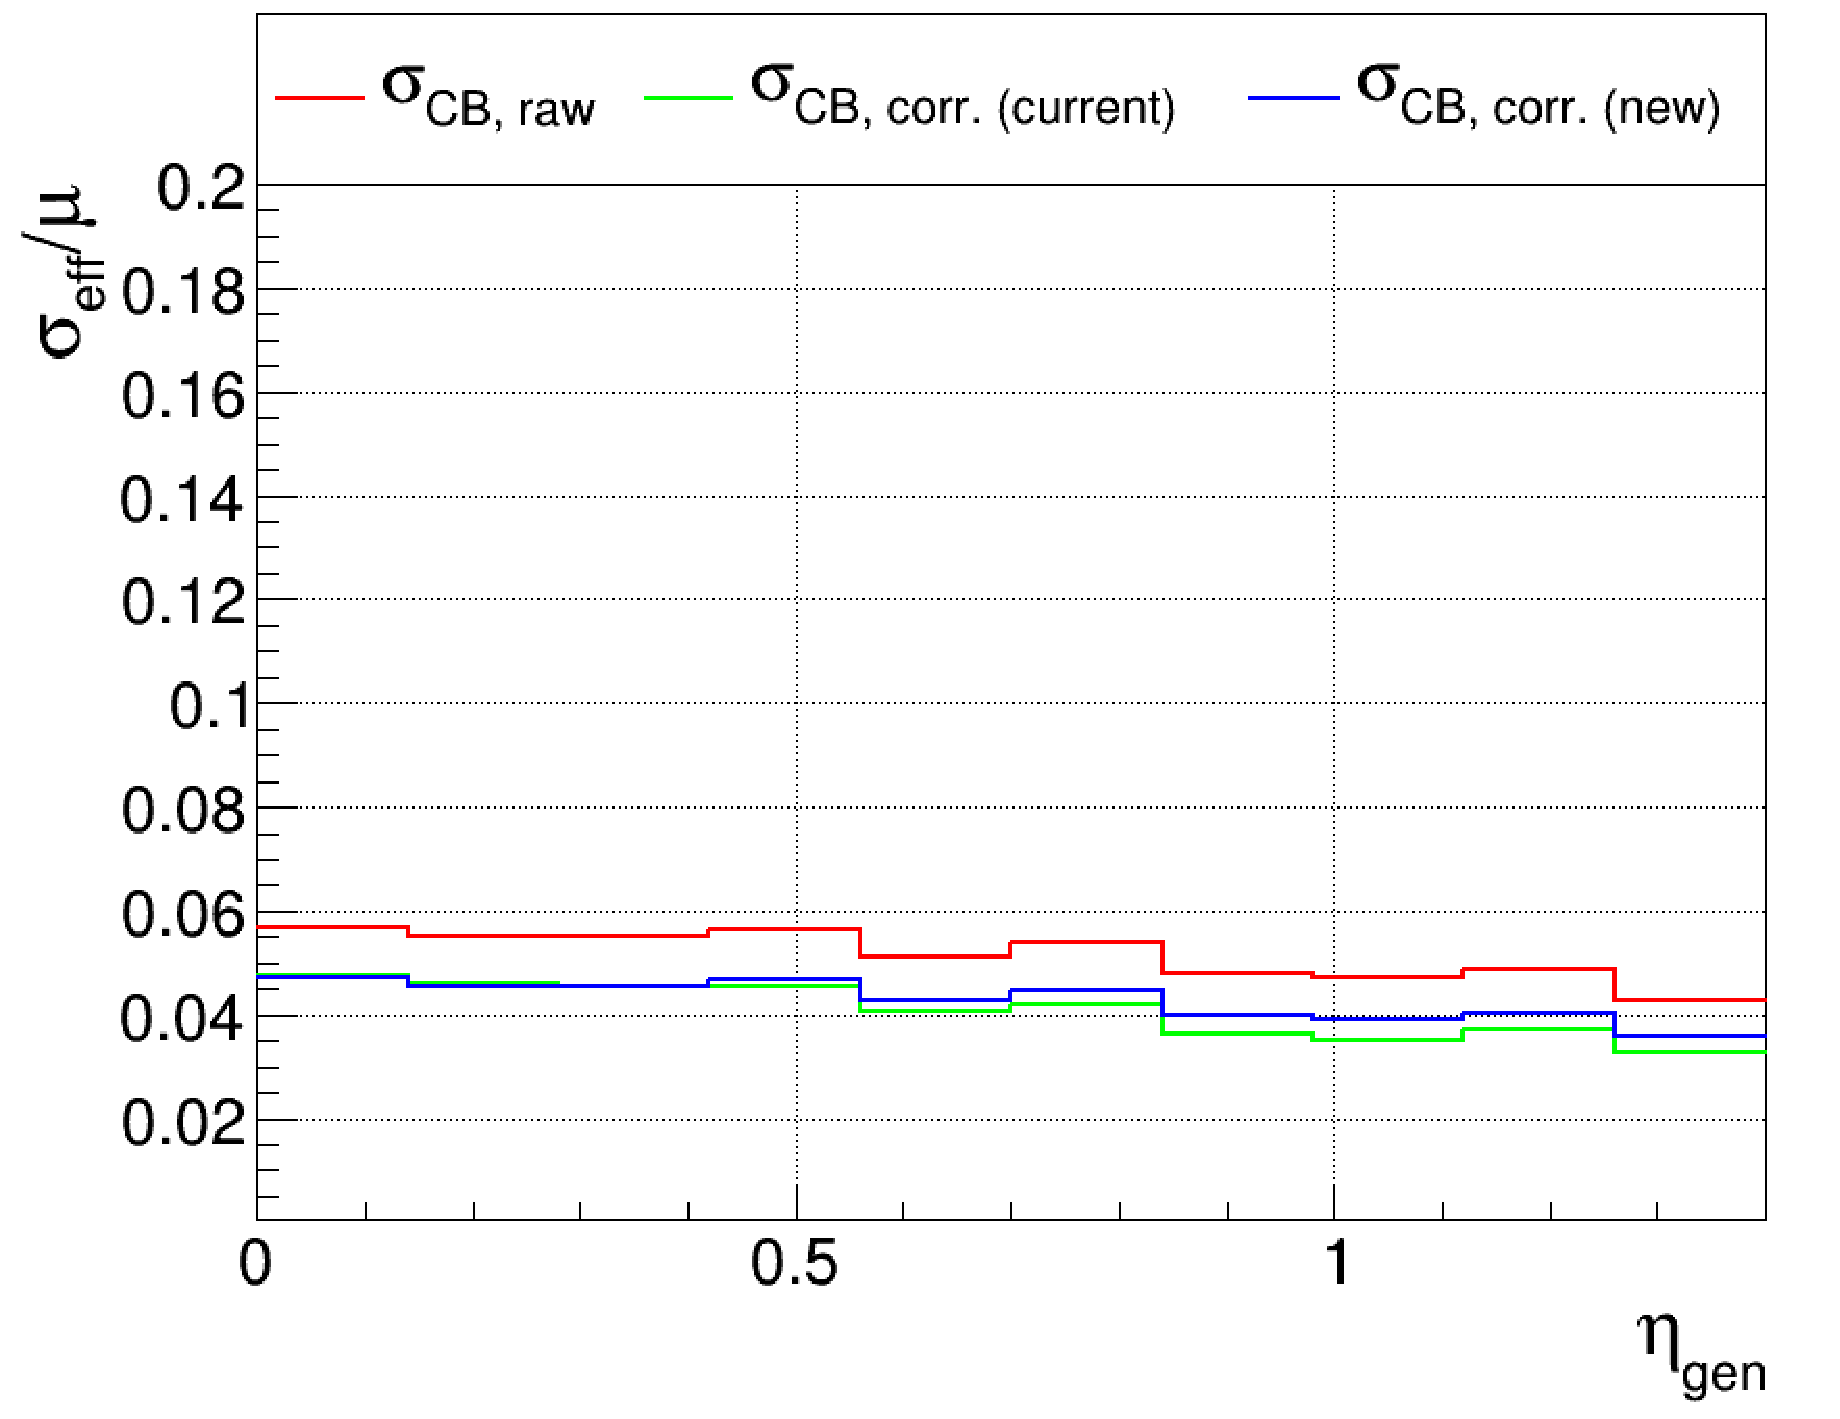
\includegraphics[width=0.495\textwidth]{./plots_pdf/ECAL_plots/plotsPU/EB/FULL/pdf/GENETA/EBFULL_GENETA_0005_0020_EffSigmaOverBins.pdf}
\caption{EB - Full Readout \pt 5--20\GeV.}
\end{figure}


\begin{figure}
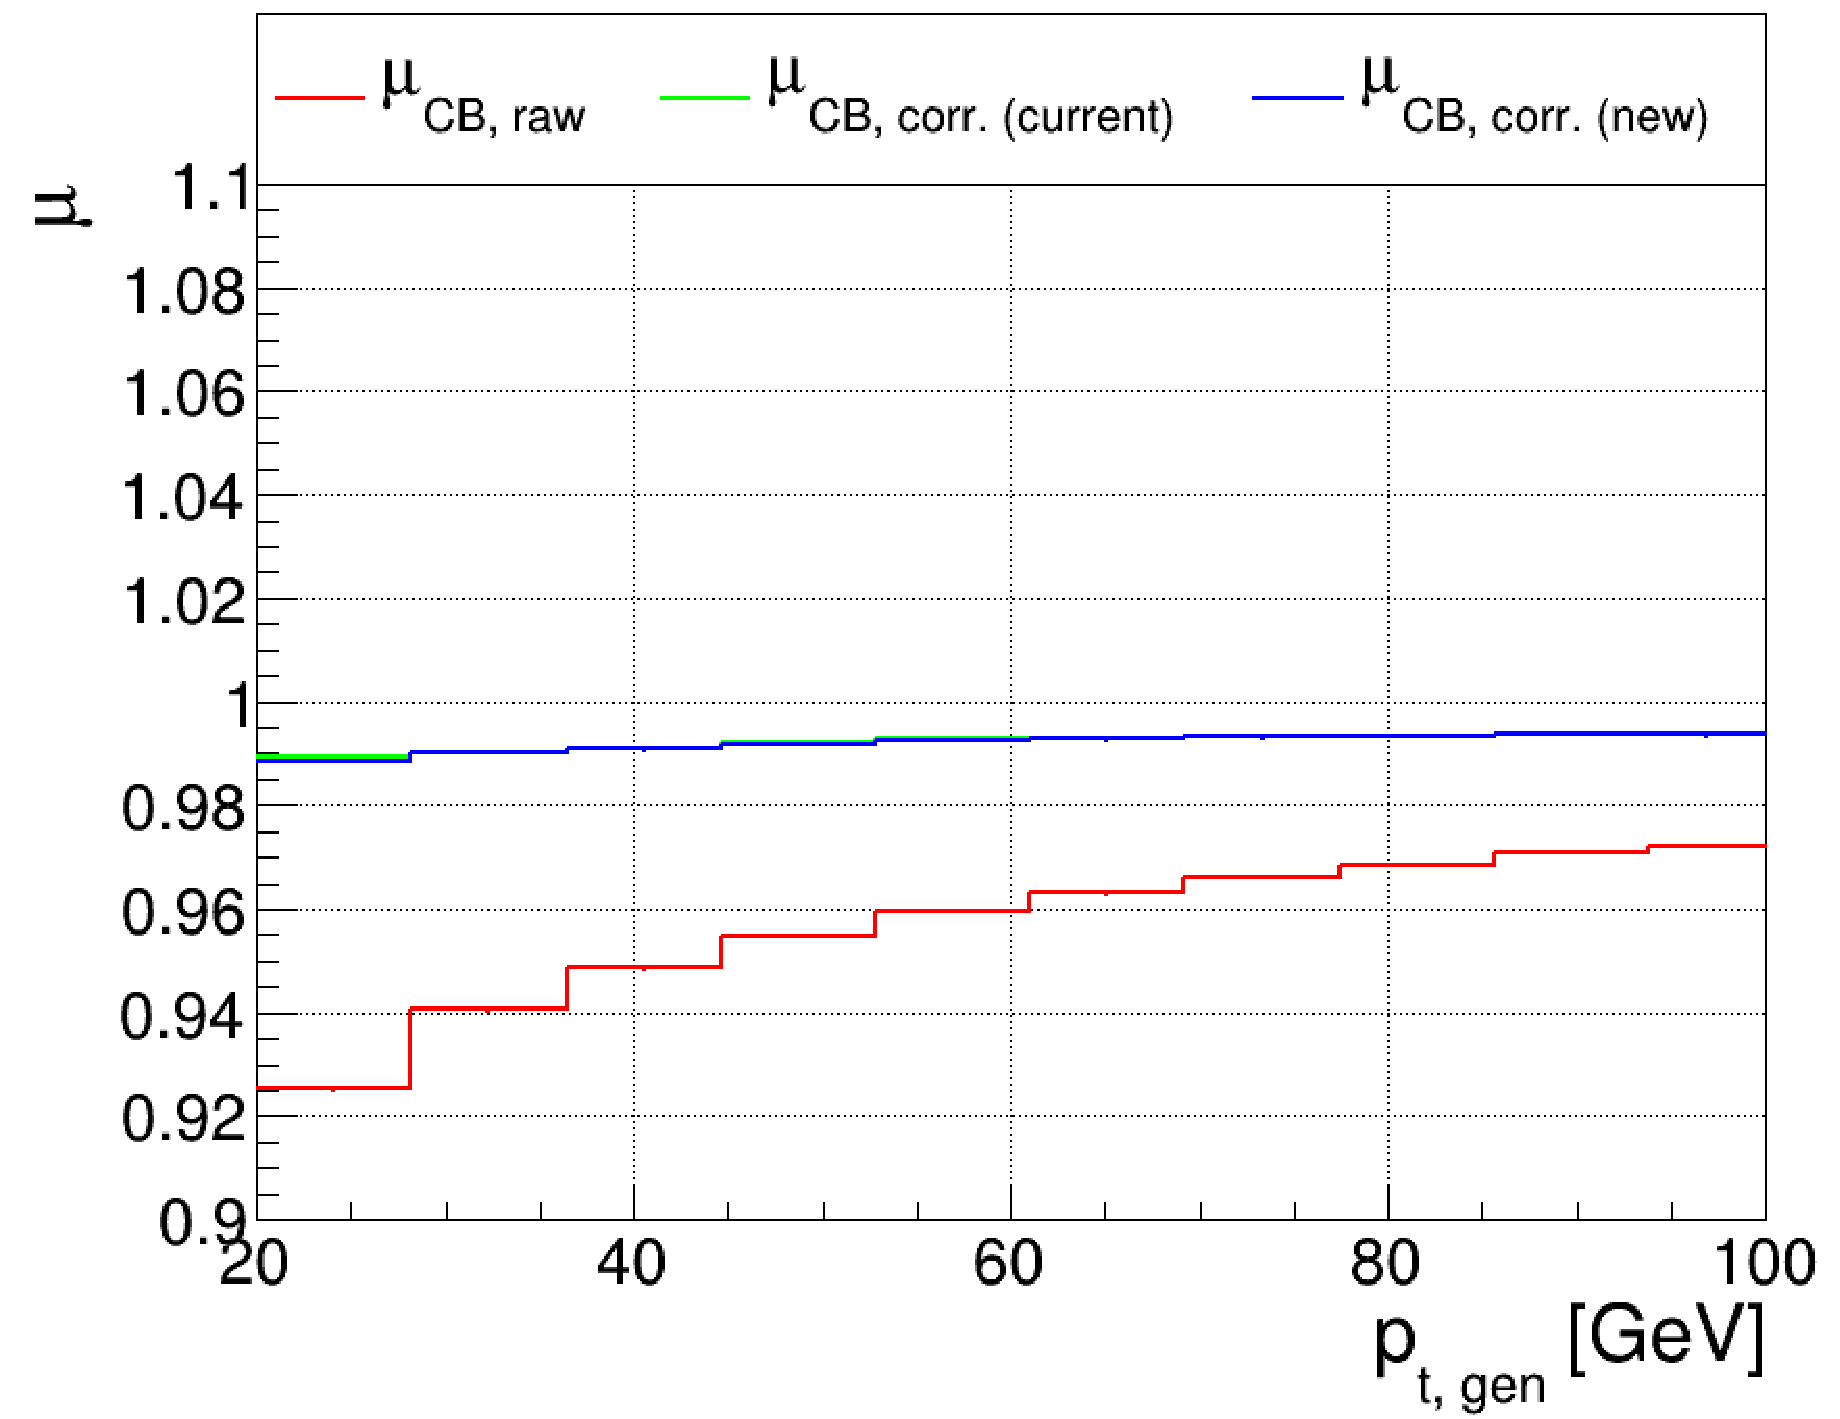
\includegraphics[width=0.495\textwidth]{./plots_pdf/ECAL_plots/plotsPU/EB/FULL/pdf/GENPT/EBFULL_GENPT_0020_0100_MuOverBins.pdf}
\includegraphics[width=0.495\textwidth]{./plots_pdf/ECAL_plots/plotsPU/EB/FULL/pdf/GENPT/EBFULL_GENPT_0020_0100_EffSigmaOverBins.pdf}
%\caption{EB - Full Readout pt 20-100}
%\end{figure}
%\begin{figure}
\includegraphics[width=0.495\textwidth]{./plots_pdf/ECAL_plots/plotsPU/EB/FULL/pdf/GENETA/EBFULL_GENETA_0020_0100_MuOverBins.pdf}
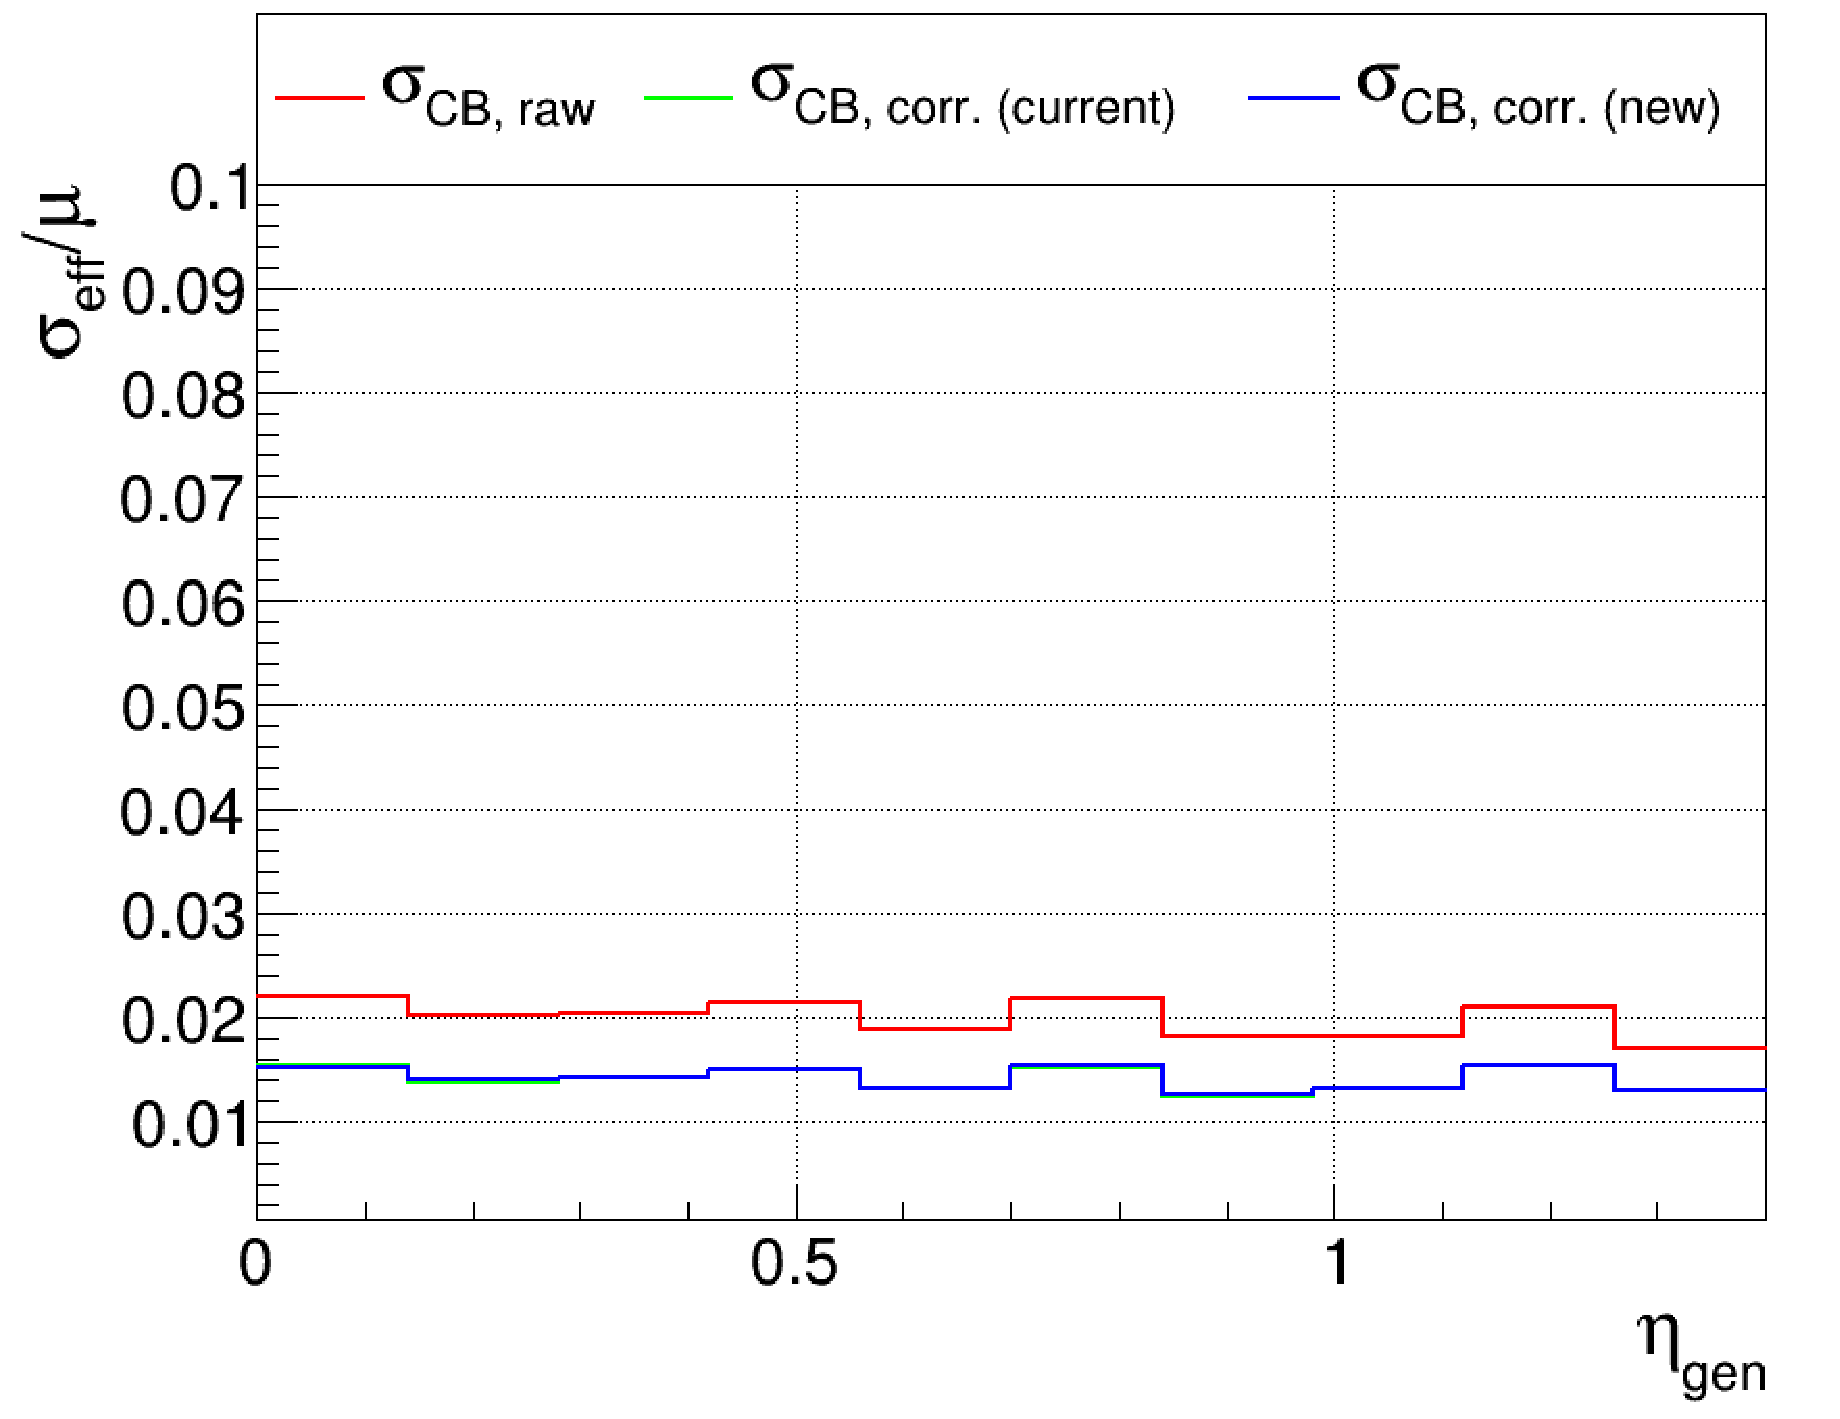
\includegraphics[width=0.495\textwidth]{./plots_pdf/ECAL_plots/plotsPU/EB/FULL/pdf/GENETA/EBFULL_GENETA_0020_0100_EffSigmaOverBins.pdf}
\caption{EB - Full Readout \pt 20--100\GeV.}
\end{figure}

\begin{figure}
\includegraphics[width=0.495\textwidth]{./plots_pdf/ECAL_plots/plotsPU/EB/FULL/pdf/GENPT/EBFULL_GENPT_0100_0300_MuOverBins.pdf}
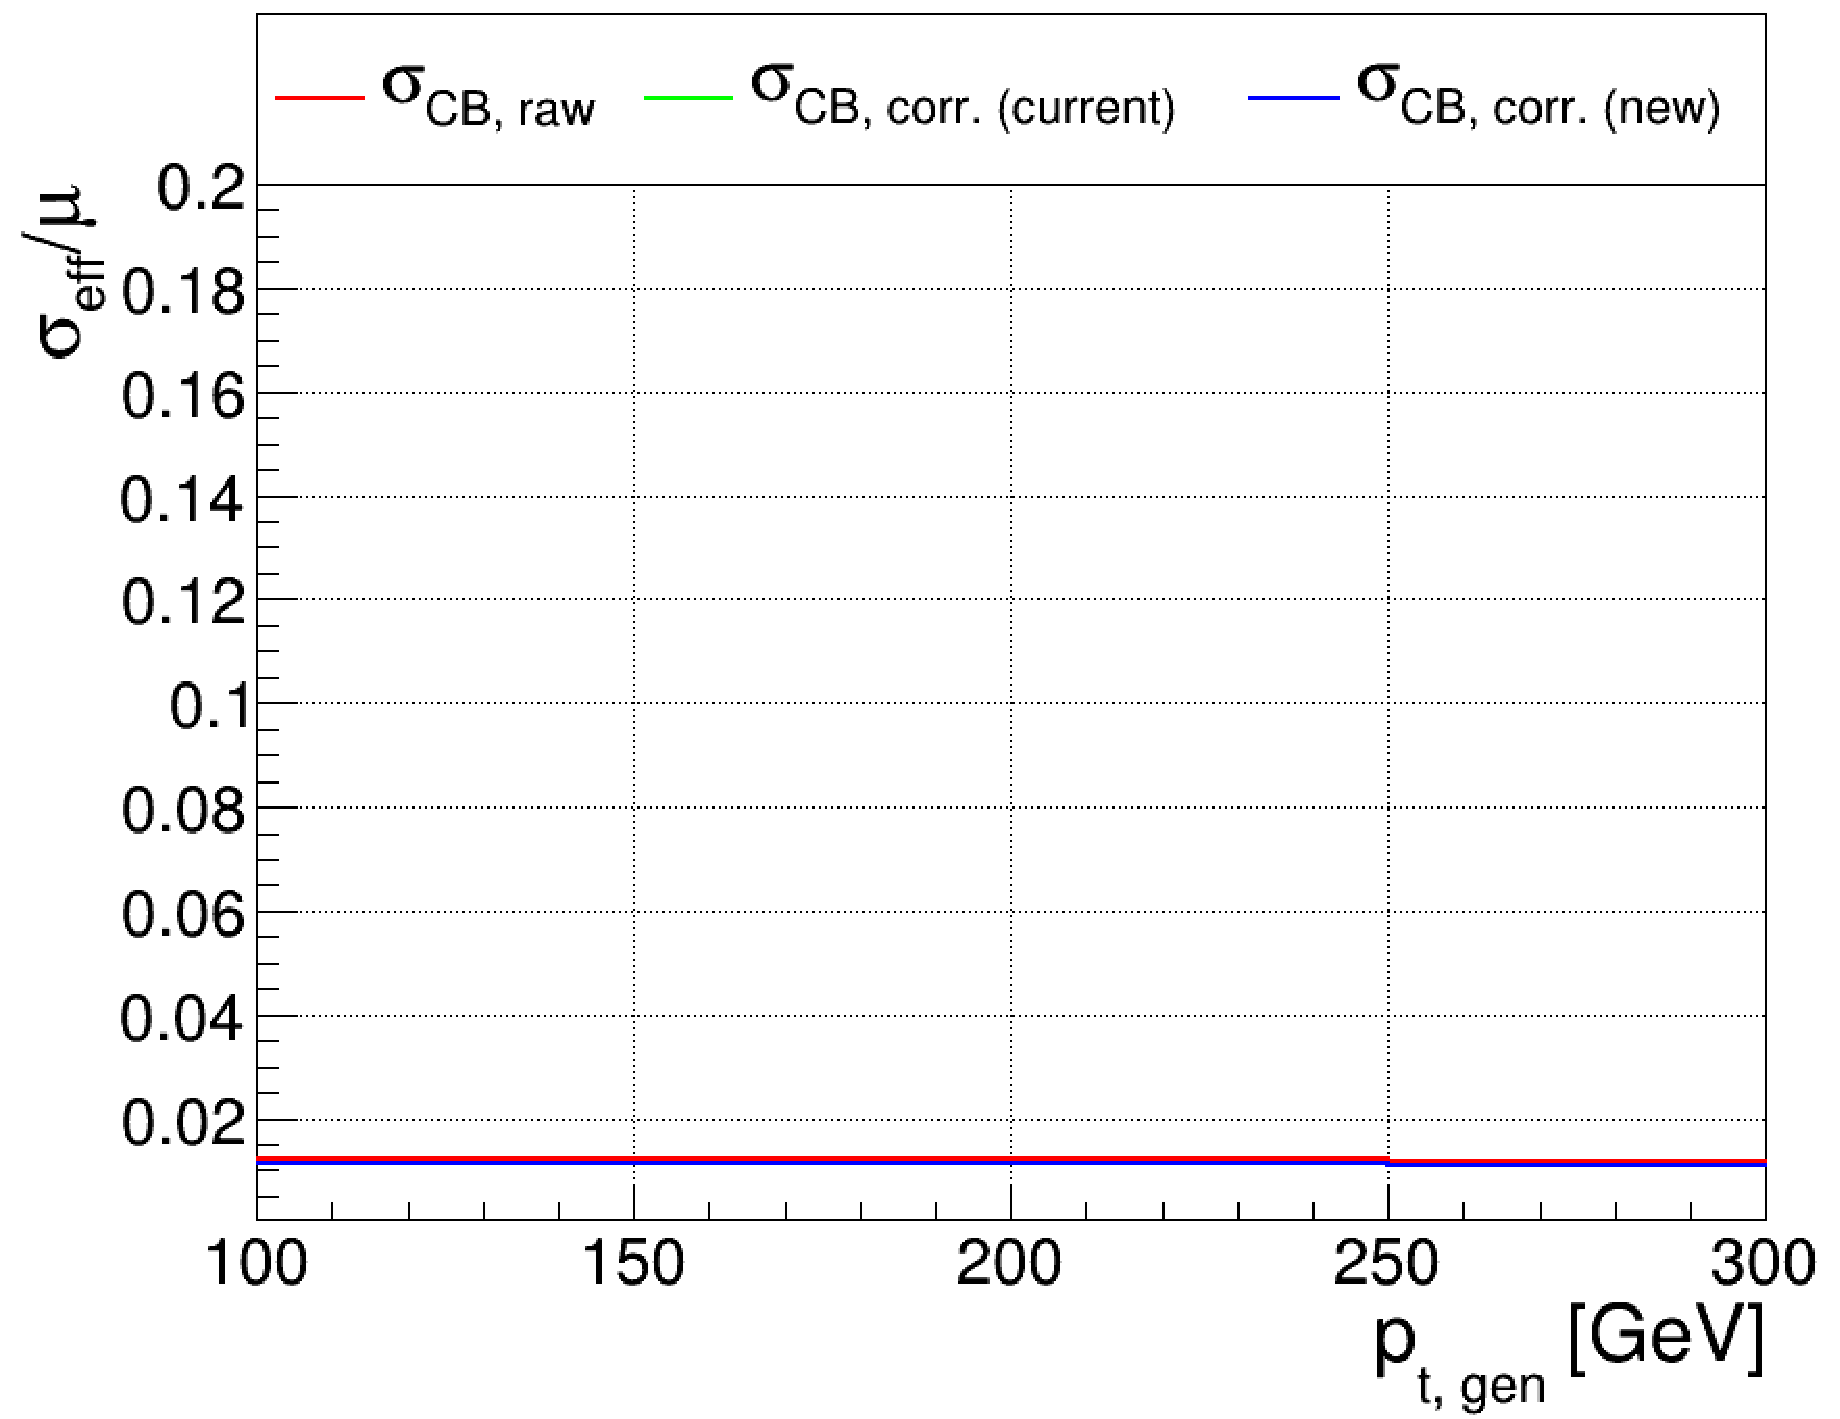
\includegraphics[width=0.495\textwidth]{./plots_pdf/ECAL_plots/plotsPU/EB/FULL/pdf/GENPT/EBFULL_GENPT_0100_0300_EffSigmaOverBins.pdf}
%\caption{EB - Full Readout pt 100-300}
%\end{figure}
%\begin{figure}
\includegraphics[width=0.495\textwidth]{./plots_pdf/ECAL_plots/plotsPU/EB/FULL/pdf/GENETA/EBFULL_GENETA_0100_0300_MuOverBins.pdf}
\includegraphics[width=0.495\textwidth]{./plots_pdf/ECAL_plots/plotsPU/EB/FULL/pdf/GENETA/EBFULL_GENETA_0100_0300_EffSigmaOverBins.pdf}
\caption{EB - Full Readout \pt 100-300\GeV}
\end{figure}





\begin{figure}
\includegraphics[width=0.495\textwidth]{./plots_pdf/ECAL_plots/plotsPU/EB/ZS/pdf/GENPT/EBZS_GENPT_0000_0006_MuOverBins.pdf}
\includegraphics[width=0.495\textwidth]{./plots_pdf/ECAL_plots/plotsPU/EB/ZS/pdf/GENPT/EBZS_GENPT_0000_0006_EffSigmaOverBins.pdf}

\includegraphics[width=0.495\textwidth]{./plots_pdf/ECAL_plots/plotsPU/EB/ZS/pdf/GENETA/EBZS_GENETA_0000_0006_MuOverBins.pdf}
\includegraphics[width=0.495\textwidth]{./plots_pdf/ECAL_plots/plotsPU/EB/ZS/pdf/GENETA/EBZS_GENETA_0000_0006_EffSigmaOverBins.pdf}
\caption[$\mu$ ($\sigma_\mathrm{eff}$) vs \pt of PF ECAL cluster - EB ZS readout PU  senario]{Mean response (resolution) defined by Raw PF ECAL clusters (red), the calibration derived earlier in Ru\
n3 based on 126X (green), and the new correction from 2024 simulation sample based on 133X (blue). \pt 0--6\GeV PU EB ZS readout PU senario.}
\label{fig:PU_EBZS}
\end{figure}

%% %\begin{figure}
%% \includegraphics[width=0.495\textwidth]{./plots_pdf/ECAL_plots/plotsPU/EB/ZS/pdf/GENPT/EBZS_GENPT_0006_0025_MuOverBins.pdf}
%% \includegraphics[width=0.495\textwidth]{./plots_pdf/ECAL_plots/plotsPU/EB/ZS/pdf/GENPT/EBZS_GENPT_0006_0025_EffSigmaOverBins.pdf}
%% %\caption{EB - ZS Readout pt 6-25}
%% %\end{figure}
%% %\begin{figure}
%% \includegraphics[width=0.495\textwidth]{./plots_pdf/ECAL_plots/plotsPU/EB/ZS/pdf/GENETA/EBZS_GENETA_0006_0025_MuOverBins.pdf}
%% \includegraphics[width=0.495\textwidth]{./plots_pdf/ECAL_plots/plotsPU/EB/ZS/pdf/GENETA/EBZS_GENETA_0006_0025_EffSigmaOverBins.pdf}
%% \caption{EB - ZS Readout \pt 6-25}
%% \end{figure}






\begin{figure}
\includegraphics[width=0.495\textwidth]{./plots_pdf/ECAL_plots/plotsPU/EE/FULL/pdf/GENPT/EEFULL_GENPT_0005_0020_MuOverBins.pdf}
\includegraphics[width=0.495\textwidth]{./plots_pdf/ECAL_plots/plotsPU/EE/FULL/pdf/GENPT/EEFULL_GENPT_0005_0020_EffSigmaOverBins.pdf}
\includegraphics[width=0.495\textwidth]{./plots_pdf/ECAL_plots/plotsPU/EE/FULL/pdf/GENPT/EEFULL_GENPT_0020_0100_MuOverBins.pdf}
\includegraphics[width=0.495\textwidth]{./plots_pdf/ECAL_plots/plotsPU/EE/FULL/pdf/GENPT/EEFULL_GENPT_0020_0100_EffSigmaOverBins.pdf}
\includegraphics[width=0.495\textwidth]{./plots_pdf/ECAL_plots/plotsPU/EE/FULL/pdf/GENPT/EEFULL_GENPT_0100_0300_MuOverBins.pdf}
\includegraphics[width=0.495\textwidth]{./plots_pdf/ECAL_plots/plotsPU/EE/FULL/pdf/GENPT/EEFULL_GENPT_0100_0300_EffSigmaOverBins.pdf}

\caption [$\mu$ ($\sigma_\mathrm{eff}$) vs \pt of PF ECAL cluster - EE full readout PU scenario]{Mean response (resolution) defined by Raw PF ECAL clusters (red), the calibration derived earlier in Ru\
n3 based on 126X (green), and the new correction from 2024 simulation sample based on 133X (blue). (top) low \pt, (middle) mid \pt, (bottom) high \pt in EE region full readout PU scenario.}
\label{fig:PU_EEFULL_pt}
\end{figure}


\begin{figure}
\includegraphics[width=0.495\textwidth]{./plots_pdf/ECAL_plots/plotsPU/EE/FULL/pdf/GENETA/EEFULL_GENETA_0005_0020_MuOverBins.pdf}
\includegraphics[width=0.495\textwidth]{./plots_pdf/ECAL_plots/plotsPU/EE/FULL/pdf/GENETA/EEFULL_GENETA_0005_0020_EffSigmaOverBins.pdf}
\includegraphics[width=0.495\textwidth]{./plots_pdf/ECAL_plots/plotsPU/EE/FULL/pdf/GENETA/EEFULL_GENETA_0020_0100_MuOverBins.pdf}
\includegraphics[width=0.495\textwidth]{./plots_pdf/ECAL_plots/plotsPU/EE/FULL/pdf/GENETA/EEFULL_GENETA_0020_0100_EffSigmaOverBins.pdf}
\includegraphics[width=0.495\textwidth]{./plots_pdf/ECAL_plots/plotsPU/EE/FULL/pdf/GENETA/EEFULL_GENETA_0100_0300_MuOverBins.pdf}
\includegraphics[width=0.495\textwidth]{./plots_pdf/ECAL_plots/plotsPU/EE/FULL/pdf/GENETA/EEFULL_GENETA_0100_0300_EffSigmaOverBins.pdf}


\caption [$\mu$ ($\sigma_\mathrm{eff}$) vs $\eta$ of PF ECAL cluster - EE Full readout PU scenario]{Mean response (resolution) defined by Raw PF ECAL clusters (red), the calibration derived earlier in\
 Run3 based on 126X (green), and the new correction from 2024 simulation sample based on 133X (blue). (top) low $\eta$, (middle) mid $\eta$, (bottom) high $\eta$ in EE region Full readout PU scenario.}
\label{fig:PU_EEFULL_eta}
\end{figure}

\begin{figure}
\includegraphics[width=0.495\textwidth]{./plots_pdf/ECAL_plots/plotsPU/EE/ZS/pdf/GENPT/EEZS_GENPT_0000_0006_MuOverBins.pdf}
\includegraphics[width=0.495\textwidth]{./plots_pdf/ECAL_plots/plotsPU/EE/ZS/pdf/GENPT/EEZS_GENPT_0000_0006_EffSigmaOverBins.pdf}

\includegraphics[width=0.495\textwidth]{./plots_pdf/ECAL_plots/plotsPU/EE/ZS/pdf/GENETA/EEZS_GENETA_0000_0006_MuOverBins.pdf}
\includegraphics[width=0.495\textwidth]{./plots_pdf/ECAL_plots/plotsPU/EE/ZS/pdf/GENETA/EEZS_GENETA_0000_0006_EffSigmaOverBins.pdf}

\caption[$\mu$ ($\sigma_\mathrm{eff}$) vs. \pt of PF ECAL cluster - EE ZS readout PU scenario]{Mean response (resolution) defined by raw PF ECAL clusters (red), the calibration derived earlier in Run~3 based on 126X (green), and the new correction from the 2024 simulation sample based on 133X (blue).\pt 0--6\GeV in EE region ZS readout PU scenario.}
\label{fig:PU_EEZS}
\end{figure}

%% %\begin{figure}
%% \includegraphics[width=0.495\textwidth]{./plots_pdf/ECAL_plots/plotsPU/EE/ZS/pdf/GENPT/EEZS_GENPT_0006_0025_MuOverBins.pdf}
%% \includegraphics[width=0.495\textwidth]{./plots_pdf/ECAL_plots/plotsPU/EE/ZS/pdf/GENPT/EEZS_GENPT_0006_0025_EffSigmaOverBins.pdf}
%% %\caption{EE - ZS Readout pt 6-25}
%% %\end{figure}
%% %\begin{figure}
%% \includegraphics[width=0.495\textwidth]{./plots_pdf/ECAL_plots/plotsPU/EE/ZS/pdf/GENETA/EEZS_GENETA_0006_0025_MuOverBins.pdf}
%% \caption{EE - ZS Readout \pt 6-25}
%% \end{figure}









HLT vs offline PF ECAL cluster
first for NoPU samples




%%%%%%%%%%%%%%%%%%%%%%%%%%%%%%%%%%%%%%%%%%%%%%%                                                                                                                                     
\begin{figure}
\includegraphics[width=0.495\textwidth]{./ECAL_plots/Prod6/NoPU/H_GenPi_Pt_vs_RespE.pdf}
%\caption{(PF cluster offline E / PFC online E) vs pt}
\includegraphics[width=0.495\textwidth]{./ECAL_plots/Prod6/NoPU/H_GenPi_Eta_vs_RespE.pdf}
\caption{(PF cluster offline E / PFC online E)}
\end{figure}

\begin{figure}
\includegraphics[width=0.495\textwidth]{./ECAL_plots/Prod6/NoPU/H_GenPi_Pt_vs_RespCE.pdf}
%\caption{(PF cluster offline E corrected / PFC online E corrected) vs pt}
\includegraphics[width=0.495\textwidth]{./ECAL_plots/Prod6/NoPU/H_GenPi_Eta_vs_RespCE.pdf}
\caption{(PF cluster offline E corrected / PFC online E corrected)}
\end{figure}                                                                                                                                                                       
%%%%%%%%%%%%%%%%%%%%%%%%%%%%%%%%%%%%%%%%%%%%%%%%                                                                                                                                    


Second for PUU samples
\begin{figure}
\includegraphics[width=0.495\textwidth]{./plots_pdf/ECAL_plots/Prod6/PU/H_GenPi_Pt_vs_RespE.pdf}
%\caption{(PF cluster offline E / PFC online E) vs pt}                                                                 
\includegraphics[width=0.495\textwidth]{./plots_pdf/ECAL_plots/Prod6/PU/H_GenPi_Eta_vs_RespE.pdf}
\caption{(PF cluster offline E / PFC online E)}
\label{fig:PU_ECAL_Offline_vs_Online_E}
\end{figure}

\begin{figure}
\includegraphics[width=0.495\textwidth]{./plots_pdf/ECAL_plots/Prod6/PU/H_GenPi_Pt_vs_RespCE.pdf}
%\caption{(PF cluster offline E corrected / PFC online E corrected) vs pt}                                             
\includegraphics[width=0.495\textwidth]{./plots_pdf/ECAL_plots/Prod6/PU/H_GenPi_Eta_vs_RespCE.pdf}
\caption{(PF cluster offline E corrected / PFC online E corrected)}
\label{fig:PU_ECAL_Offline_vs_Online_CE}
\end{figure}       



%%%%%%%%%%%%%%%%%%%%%%%%%%%%%%%%%%%%%%%%%%%%%%%%
%\section{Citations}
%Here is a citation \cite{fake1}, and here is another \cite{fake2}. Citations are
%nice. Depending on your choice of bibliography, there may be different formats
%you can use. For example, Chicago provides a family of short citation commands.
